%\documentclass{article}
\documentclass{scrartcl}
\setlength{\parindent}{0in}
\makeatletter
\DeclareOldFontCommand{\rm}{\normalfont\rmfamily}{\mathrm}
\DeclareOldFontCommand{\sf}{\normalfont\sffamily}{\mathsf}
\DeclareOldFontCommand{\tt}{\normalfont\ttfamily}{\mathtt}
\DeclareOldFontCommand{\bf}{\normalfont\bfseries}{\mathbf}
\DeclareOldFontCommand{\it}{\normalfont\itshape}{\mathit}
\DeclareOldFontCommand{\sl}{\normalfont\slshape}{\@nomath\sl}
\DeclareOldFontCommand{\sc}{\normalfont\scshape}{\@nomath\sc}
\makeatother

\usepackage{multirow}

\usepackage[utf8]{inputenc}
\usepackage{amsmath}
\usepackage{amssymb}
\usepackage{lscape}

\usepackage{algorithmic}
\usepackage{algorithm}
\renewcommand{\algorithmicrequire}{\textbf{Input:}}
\renewcommand{\algorithmicensure}{\textbf{Output:}}

\usepackage{xcolor}
\usepackage{yfonts}
\usepackage[T1]{fontenc}
\usepackage[toc,page]{appendix}


\usepackage{graphicx}		 % Need this to include images
\usepackage[hidelinks]{hyperref}
\usepackage{blkarray}
\usepackage{cancel}
\usepackage{enumitem}
\usepackage{listings}
\usepackage{color}
\usepackage{pdfpages}
\usepackage{helvet}


\definecolor{dkgreen}{rgb}{0,0.6,0}
\definecolor{gray}{rgb}{0.5,0.5,0.5}
\definecolor{mauve}{rgb}{0.58,0,0.82}

\lstdefinestyle{base}{
  inputencoding=latin10,
  emptylines=1,
  breaklines=true,
  basicstyle=\small\ttfamily,
  moredelim=**[is][\color{red}]{@}{@},
}

\newcommand{\norm}[1]{\left\lVert#1\right\rVert}

%% Define a HUGE 
\makeatletter
\newcommand\HUGE{\@setfontsize\Huge{24.88}{50}}
\makeatother

\begin{document}             % End of preamble and beginning of text.

 
%titlepage
\thispagestyle{empty}
\begin{center}
\begin{minipage}{.9\linewidth}
\flushright
	      		 
	%University logo
    
\includegraphics[width=0.5\linewidth]{univie.eps}\par
\centering 	
    % Title
	{\scshape{\HUGE Bachelorarbeit\par}}
	\vspace{1cm}
	%Thesis title
    {\scshape{\Large Implementation and experimental comparison between the COMMUNICATION AVOIDING-GENERALIZED MINIMAL RESIDUAL METHOD and standard GMRES \par}}
    \vspace{2cm}
    
  
 Verfasser  \linebreak
 {\Large Robert Ernstbrunner \par}
 	\vspace{.7cm}
angestrebter akademischer Grad\linebreak
 {\Large Bachelor of Science (BSc)\par}
	\vspace{.7cm}

\flushleft
	

\begin{tabular}{ll}
Wien, 2019	\linebreak
\vspace{.5cm}&   \\
  Studienkennzahl lt. Studienblatt: & A 033 521 \vspace{.3cm} \\ 
  Fachrichtung: & Informatik  - Scientific Computing
  \vspace{.3cm} \\
  Betreuerin / Betreuer: & Univ.-Prof. Dipl.-Ing. Dr.\\ 
  & Wilfried Gansterer, M.Sc. \\
 \end{tabular}
 

\end{minipage}
\end{center}
\clearpage

\pagebreak

\tableofcontents

\pagebreak

\section{Notation}
For linear algebra, similar notation is considered as in \cite{Hoemmen:2010:CKS:1970638} and \cite{Grigori}.
\begin{itemize}
\item Greek letters denote scalars, lower case Roman letters denote vectors (or - based on the context - dimensions), capital Roman letters denote matrices.
\item Capital letters with two subscripts, e.g. '$V_{m, n}$', denote matrices with $m$ rows and $n$ columns.
\item Capital \textit{Black letter} letters (e.g. $V$, $Q$ and $R$ in Black letters are represented by $\frak{V}$, $\frak{Q}$ and $\frak{R}$ resp.) denote matrices that are composed out of other matrices. 
\item $v_k$ denotes the $k^{th}$ vector in a series of vectors $v_0$, $v_1$, $\ldots$, ,  $v_k$, $v_{k+1}$, $\ldots$ of equal length.
\item Similarly, $V_k$ denotes the $k^{th}$ matrix in a sequence of matrices $V_0$, $V_1$, $\ldots$ , $V_k$, $V_{k+1}$, $\ldots$. Generally all these matrices have the same number of rows. They may or may not have the same number of columns.
\item If $V_k$ is a matrix consisting of $s$ vectors $\left[v_1, v_2, \ldots, v_s\right]$, $\underline{V}_k$ comprises vectors $\left[V_k, v_{s+1} \right]$. The underline means one more column at the end.
\item If again, $V_k$ is a matrix consisting of $s$ vectors $\left[v_1, v_2, \ldots, v_s\right]$, $\acute{V}$ consists of vectors $[v_2, v_3, \ldots, v_s]$. The acute denotes one column less at the beginning.
\item As a consequence $\underline{\acute{V}}$ denotes one more column at the end and one less column at the beginning, e.g. $\underline{\acute{V}} = [\acute{V}, v_{s+1}]$.
\item Depending on the context, both underline or/and acute letters can also refer to rows as well. 
\item $0_{m, n}$ is defined as an $m \times n$ matrix consisting of zeros and $e_k$ denotes the $k^{\text{th}}$ canonical vector with the dimension depending on the context.
\item Matlab notation is used for addressing elements of matrices and vectors. For example, given a matrix $A$ of size $n \times n$ and two sets of indices $\alpha$ and $\beta$, $A(\alpha,:)$ is a submatrix formed by the subset of the rows of $A$ whose indices belong to $\alpha$. Similarly, $A(\alpha, \beta)$ is a submatrix formed by the subset of the rows of $A$ whose indices belong to $\alpha$ and the subset of the columns of $A$ whose indices belong to $\beta$.

\end{itemize}
\pagebreak

\begin{abstract}
Abstract
\end{abstract}
\section{Introduction}
As the CPU-memory performance gap widens the cost for communication increases as well.

Compared to arithmetic costs communication costs are much higher and the widening CPU-memory performance gap promotes the need for communication-avoiding algorithms.\\

The CA-GMRES algorithm was implemented in a shared-memory environment.

Communication avoiding GMRES is based on s-step GMRES 
\cite{Erhel95aparallel}

\section{Related work}
s-step methods, CA-ILU(0)

\section{Computational kernels}
%introduction; definitions: kernel, communication-avoiding
In this thesis \textit{computational kernels} define the parts of an algorithm with the highest costs. These costs include both arithmetic operations and communication.
The term \textit{communication} generally denotes the movement of data either between different processors in the parallel case or between 'fast' and 'slow' memory in the sequential case, where 'fast' and 'slow' are relative to the two levels examined in the memory hierarchy (e.g. cache and DRAM, or DRAM and disk). Communication optimal algorithms do not eliminate communication completely, but they are constructed in a way such that reduction of communication is prioritized. This often results in new challenges, e.g., the  CA-ILU(0) algorithm (section~\ref{sec:ca-ilu}) has to balance between communication and redundant computations; CA-GMRES (section~\ref{sec:ca-gmres}) incorporates additional techniques to deal with ill-conditioned basis vectors.

\subsection{Matrix powers kernel (MPK)}
\cite{Hoemmen:2010:CKS:1970638} p.60\\
The Matrix Powers Kernel 
Power iteration, SpMV instead of MV, sparse matrix like a graph $\rightarrow$ spacial, temporal locality not as efficiently used as in dense MV. 
Avoid communication by sending / receiving all necessary values beforehand (look at reachability of graph(A)) and computing s basis vectors without further communication.\\


Although, the matrix powers kernel was not implemented in the context of this thesis it is still an essential kernel to avoid communication and therefore, will be briefly summarized here.
The matrix powers kernel replaces the sparse matrix-vector products that generate the basis for the Krylov subspace $\mathcal{K}_m(A, v) = \left[v, Av, A^2v, \ldots, A^{m-1}v\right]$. One invocation of the MPK produces the same amount of basis vectors as $s$ sparse matrix-vector products. The data and the workload are partitioned among $P$ processors, where each processor gets $A(\alpha,:)$ and $v_0(\alpha)$ with $\alpha$ being the subset assigned to the specific processor. by a factor $\Theta(s)$ and the matrix has to be loaded from slow to fast memory only once instead of $s$.  than  each processor is assigned a part $\alpha$ of the input vector $v_0$ and $A(\alpha,:)$.


\texttt{To minimize communication in a parallel setting, the s monomial basis vectors of the Krylov subspace $[y, Ay, A2y, \ldots, A^sy]$ are computed with no communication using the so-called matrix powers kernel [13]. This requires ghosting and computing redundantly on each processor the data required for computing its part of the vectors with no communication. Note that throughout this paper we use the term ghosting to denote the storage of redundant data, of vectors or matrices, that do not belong to the processor's assigned domain or part, but are needed for future computations.\\
First, the data and the work is split between $P$ processors. Each processor is assigned a part $\alpha$ of the input vector $y_0$ ($y_0(\alpha)$) and $A(\alpha, :)$, where $\alpha \subseteq V(G(A))$. Then, each processor has to compute the same part $\alpha$ of $y_1 = Ay_0$, $y_2 = Ay_1$, till $y_s = Ay_{s - 1}$ without communicating with other processors. To do so, each 
processor fetches all the data needed from the neighboring processors, to compute its part $\alpha$ of the $s$ vectors. Thus, to compute $y_s(\alpha)$, each processor should receive the missing data of $y_0(\eta_s)$ and $A(\eta_s, :)$ from its neighboring processors and store it redundantly, where $\eta_s = R(G(A), \alpha, s)$. Finally, each processor computes the set $R(G(A), \alpha, s - i)$ of the vectors $y_i$ for $i = 1, 2, \ldots, s$ without any communication with the other processors.}


\subsection{Tall and skinny QR (TSQR)}
Unconditionally stable like Householder QR but less communication

\subsection{Block Classical Gram-Schmidt (BCGS)}
Dense matrix-matrix multiplications $\rightarrow$ less communication (factor $\Theta(s)$ fewer messages) than unblocked CGS. Also, BCGS requires less communication that BMGS.
No reorthogonalization because solving linear system with (std. GMRES uses unblocked MGS-Arnoldi) CA-GMRES uses TSQR which improves orthogonality of the block columns.

\section{Arnoldi iteration}

first presented in \textit{REF[[ W. E. Arnoldi, The principle of minimized iterations in the solution of the matrix eigenvalue problem, Q. Appl. Maths, 9 (1951), pp. 17–29.]]}\\

s steps of standard Arnoldi produce an $s + 1 \times s$ upper Hessenberg Matrix $\underline{H}$ and $m \times s + 1$ orthonormal vectors $q_1$, $q_2$, $\ldots$, $q_s$, $q_{s + 1}$ that form a basis for the Krylov subspace $\mathcal{K}_{s + 1}\left(A,r\right)$ such that $AQ = \underline{Q} \underline{H}$. There are many ways to orthogonalize successive basis vectors. Modified Gram-Schmidt (MGS) is often employed because it provides high numerical stability, however, although not as stable, Classical Gram-Schmidt (CGS) is more suited for parallel implementations because it provides fewer synchronization points.

introduction.. produces $AQ = QH$
\subsection{Arnoldi(s)}

[238] H. F. Walker, Implementation of the GMRES and Arnoldi methods using Householder transformations, Tech. Rep. UCRL-93589, Lawrence Livermore National Laboratory, Oct. 1985.

source above! \texttt{At the heart of Arnoldi’s method is a Gram-Schmidt process, and so we refer to the
GMRES implementation of [8] as the Gram-Schmidt implementation. The basic form
of Arnoldi’s method given above employs the classical Gram-Schmidt process, which
is numerically untrustworthy. Because of roundoff, there may be severe loss of orthogonality among the computed Vm’S. In practice, it is usual to implement Arnoldi’s
method using the modified Gram-Schmidt process (see Golub and Van Loan [4]).
Mathematically, this is just a rearrangement of the classical process; computationally, it has superior properties.
Even the modified Gram-Schmidt process can fail to perform well if the vectors on which it operates are not sufficiently independent. Indeed, if S (sl,... ,sin) is an n m matrix the columns of which are to be orthonormalized and if Q (ql,. qm) is the computed result of applying modified Gram-Schmidt to the columns of S using floating point arithmetic with unit rounding error u, then Bjorck [1] has shown that (1.6) QTQ I + E, [IEll2 where the condition number 2(S) is the ratio of the largest singular value of S to the smallest. It follows that at the mth step of Arnoldi’s method using modified GramSchmidt, Vm+ may have a significantly nonzero conponent in the span of {vl,. Vm}
if 2((vl,...,vm,Avm)) is large, i. e., if Avm is nearly in the span of {vl,...,Vm}.
Shad [7, p. 214 has suggested that the Gram-Schmidt process in Arnoldi’s method may be an important source of errors in the full and incomplete orthogonalization
methods ([6],[7]), which are related to GMRES.
}

\subsubsection{The Monomial basis}
The Monomial basis in s-step Krylov methods is given by 
\begin{equation*}
\mathcal{K}_{s + 1}(A, v) = [v, Av, A^2v, \ldots, A^sv]
\end{equation*}
and has a change of basis matrix
\begin{equation*}
\underline{B} = [\sigma_1 e_2, \sigma_2 e_3, \ldots, \sigma_s e_{s + 1}].
\end{equation*}
with scaling factors $\sigma_1, \ldots, \sigma_s$.
The Monomial basis is also known as the \textit{power method} which is an iterative method for finding the principal eigenvalue and corresponding eigenvector of a matrix by repeatedly applying a starting vector to the matrix. If the matrix and starting vector satisfy certain conditions, the basis converges to the principal eigenvector. In theory, the basis is still linearly independent in exact arithmetic. In machine precision they become inevitably dependent at a certain point. \\

scaling the rapidly growing condition number and vector length $\rightarrow$ scale vector to lengh 1, but:  $\rightarrow$ need a different basis.
\subsubsection{The Newton basis}
The Newton basis in s-step Krylov methods is given by 
\begin{equation*}
\mathcal{K}_{s + 1}(A, v) = \left[v, (A - \theta_1 I )v, (A - \theta_2 I )(A - \theta_1 I )v, \ldots, \displaystyle\prod_{i = 1}^s (A - \theta_i I )v\right]
\end{equation*}
and has a change of basis matrix
\begin{equation*}
\underline{B} = 
\begin{pmatrix}
\theta_1 & 0 & \ldots & 0 \\
\sigma_1 & \theta_2 & \ddots & \vdots \\
0 & \sigma_2 & \ddots & 0 \\
\vdots & \ddots & \ddots & \theta_s \\
0 & 0 & \ldots & \sigma_s 
\end{pmatrix}
\end{equation*}
with scaling factors $\sigma_1, \ldots, \sigma_s$.\\

polinomial interpolation at shifts $\theta_1$, $\theta_2$, $\ldots$, $\theta_s$.
\paragraph{Choosing the shifts}
find estimates of the eigenvalues of A (Ritz values).
\paragraph{The modified Leja ordering}

\paragraph{Avoiding complex arithmetic}
Like the eigenvalues of a real matrix, the Ritz values can also be complex conjugate pairs. The modified Leja ordering ensures that these pairs are ordered consecutively with leading positive imaginary entries, i.e. $\theta_{j + 1} = \overline{\theta}_j$ with $\Im(\theta_j) > 0$. Complex arithmetic doubles the storage and floating point operations and therefore, should be avoided. Instead of computing $v_{j + 1} = (A - \theta_j I)v_j$ and $v_{j + 2} = (A - \overline{\theta}_j I)v_{j + 1}$ like one would normally do, Bai et al. \cite{doi:10.1093/imanum/14.4.563} suggest that complex arithmetic can be avoided by setting
\begin{equation}
v_{j + 1} = (A - \Re(\theta_j) I )v_j
\end{equation}
and
\begin{equation}
v_{j + 2} = (A - \Re(\theta_j) I )v_{k + 1} + \Im(\theta_j)^2 v_j.
\end{equation}
It can easily be shown that 
\begin{eqnarray*}
v_{j + 2} &=& (A - \Re(\theta_j) I )^2v_{j} + \Im(\theta_j)^2 v_j \\
&=& (A - \overline{\theta}_j I )(A - \theta_j I )v_{j}.
\end{eqnarray*}

This also affects the change of basis matrix $\underline{B}$. If the Ritz values contain complex conjugate pairs, $\underline{B}$ is tridiagonal. E.g., if $\theta_1$ through $\theta_s$ are real, with the exception of $\theta_j$ and $\theta_{j + 1}$ being a complex conjugate pair, the change of basis matrix is given by
\begin{equation*}
\iffalse
\begin{matrix}
\ddots & \ddots & \ddots & \ddots & \\
& \sigma_{j - 1} & $\scalebox{.7}[1]{$\Re$(}$ \theta_j$\scalebox{.7}[1]{$)$}$ & $\scalebox{.7}[1]{$-\Im($}$\theta_j$\scalebox{.7}[1]{$)$}$^2 & \\
& 0 & \sigma_j & $\scalebox{.7}[1]{$\Re$(}$ \theta_{j + 1}$\scalebox{.7}[1]{$)$}$ & \\
& & 0 & \sigma_{j + 1} & \\
& & \ddots & \ddots & \ddots \\
\end{matrix}
\fi
\underline{B} =
\begin{pmatrix}
\theta_1 & 0 & \ldots & \ldots & \ldots & 0 \\
\sigma_1 & \ddots & \ddots & \ddots & \ddots & \vdots \\
0 & \ddots & $\scalebox{.7}[1]{$\Re$(}$ \theta_j$\scalebox{.7}[1]{$)$}$ & $\scalebox{.7}[1]{$-\Im($}$\theta_j$\scalebox{.7}[1]{$)$}$^2 & \ddots & \vdots \\
\vdots & \ddots & \sigma_j & $\scalebox{.7}[1]{$\Re$(}$ \theta_{j + 1}$\scalebox{.7}[1]{$)$}$ & \ddots & \vdots \\
\vdots & \ddots & \ddots & \sigma_{j + 1} & \ddots & 0 \\
\vdots & \ddots & \ddots & \ddots & \ddots & \theta_s \\
0 & \ldots & \ldots & \ldots & 0 & \sigma_s \\
\end{pmatrix}.
\end{equation*}

\subparagraph{Performance notes}
Avoiding complex arithmetic in that way necessitates an extra SpMV operation in the Newton basis which, in the worst case, leads to as many floating point operations as in the Chebychev basis. However, in their performance analysis Hoemmen et al. \cite{Hoemmen:2010:CKS:1970638} observed that the runtime of the Newton basis was still close to the runtime of the Monomial basis. \\
\cite{Hoemmen:2010:CKS:1970638} further point out that this approach might lose accuracy when $\theta_{j - 1}$ is real and $\theta_j$ and $\theta_{j + 1}$ form a complex conjugate pair with $\Re(\theta_j) = \theta_{j - 1} $. Then
\begin{eqnarray*}
v_j &=& (A - \theta_{j - 1} I )v_{j - 1} \\
v_{j + 1} &=& (A - \Re(\theta_j) I )(A - \theta_{j - 1} I )v_{j - 1} \\
		  &=& (A - \theta_{j - 1} I )^2v_{j - 1}
\end{eqnarray*}
is equivalent to computing the monomial basis with a possibly ill-conditioned  matrix $A - \theta_{j - 1} I$. This might occur if the Ritz values reside within an ellipse with a long vertical axis and very short horizontal axis.
\subsection{Arnoldi(s,t)}
\subsubsection{Introduction}
\subsubsection{Scaling the first basis vector}
Arnoldi(s,t) produces $\underline{\textfrak{Q}}$ which differs from MGS-Arnoldi $\underline{\hat{\textfrak{Q}}}$ by a unitary scaling $\underline{\Theta}$ = diag($\theta_1$, $\theta_2$, $\ldots$, $\theta_{st}$, $\theta_{st+1}$) such that $\underline{\hat{\textfrak{Q}}} = \textfrak{\underline{Q}}\underline{\Theta}$. $\rightarrow$
\begin{itemize}
\item QR factorization must not change direction of the first column
\item compute $\theta_1 = \left< r_0, q_1 \right>$ / $\beta$
\item compute $q_1$ via MGS-Arnoldi (this happens naturally when the first outer iteration is started with MGS-Arnoldi in order to compute Ritz values for the Newton basis)
\end{itemize}
\subsubsection{QR factorization update}
overlapping / non overlapping approach.

$[\underline{\frak{Q}}_0, \underline{\acute{V}}_1 ] = [\underline{\frak{Q}}_0, \underline{\acute{Q}}_1 ] \cdot 
\begin{pmatrix}
	I_{s + 1, s + 1} & \underline{\acute{\frak{R}}}_{0,1} \\
	0_{s,s + 1} & \underline{\acute{R}}_1 \\
\end{pmatrix}$ \\

BGS $\ldots$\\

Repartitioning the R factor:

\begin{eqnarray*}
\underline{\frak{R}}_k &=&
\begin{pmatrix}
	I_{sk + 1, sk + 1} & \underline{\acute{\frak{R}}}_{k - 1, k} \\
	0_{s, sk + 1} & \underline{\acute{R}}_k \\
\end{pmatrix} = 
\begin{pmatrix}
	I_{sk, sk} & \underline{\frak{R}}_{k - 1, k} \\
	0_{s + 1, sk} & \underline{R}_k \\
\end{pmatrix} \\
\frak{R}_k &=&
\begin{pmatrix}
	I_{sk + 1, sk + 1} & \acute{\frak{R}}_{k - 1, k} \\
	0_{s - 1, sk + 1} & \acute{R}_k \\
\end{pmatrix} = 
\begin{pmatrix}
	I_{sk, sk} & \frak{R}_{k - 1, k} \\
	0_{s, sk} & R_k \\
\end{pmatrix}
\end{eqnarray*}
$R_k$ and $\underline{\acute{R}}_k$ are $s \times s$ matrices, $\underline{R}_k$ is $s + 1 \times s + 1$ and $\acute{R}_k$ is $s - 1 \times s - 1$.
\subsubsection{Reconstructing the upper Hessenberg matrix}
flop optimization. how to apply Givens rotations

$AV_k = \underline{V}_k\underline{B}_k$ \\

$A [\frak{Q}_{k - 1}, V_k] = [\frak{Q}_{k - 1}, \underline{V}_k]\underline{\frak{B}}_k$ \\

where $\underline{\frak{B}}_k$ satisfies:
\begin{equation} \label{eq:B_blackletter_k_}
\underline{\frak{B}}_k = 
\begin{pmatrix}
	\frak{H}_{k - 1} & 0_{sk, s} \\
	h_{k - 1} e_1 e^T_{sk} & \underline{B}_k \\
\end{pmatrix}
\end{equation}
with $\frak{H}_0 := H_0$ \\

\begin{eqnarray*}
&A& [\underline{\frak{Q}}_{k - 1}, \acute{Q}_k] \cdot 
\begin{pmatrix}
	I_{sk + 1, sk + 1} & \acute{\frak{R}}_{k - 1, k} \\
	0_{s - 1, sk + 1} &\acute{R}_k \\
\end{pmatrix} \\
&=& [ \underline{\frak{Q}}_{k - 1}, \underline{\acute{Q}}_k ] \cdot 
\begin{pmatrix}
	I_{sk + 1, sk + 1} & \underline{\acute{\frak{R}}}_{k - 1, k} \\
	0_{s, sk + 1} & \underline{\acute{R}}_k \\
\end{pmatrix} \cdot
\begin{pmatrix}
	\frak{H}_{k - 1} & 0_{sk, s} \\
	h_{k - 1} e_1 e^T_{sk} & \underline{B}_k \\
\end{pmatrix}
\end{eqnarray*}

We have
\begin{eqnarray*}
	A [\underline{\frak{Q}}_{k - 1}, \acute{Q}_k] = [ \underline{\frak{Q}}_{k - 1}, \underline{\acute{Q}}_k ] \underline{\frak{H}}_k
\end{eqnarray*}
therefore,
\begin{eqnarray*}
	\underline{\frak{H}}_k = 
	\begin{pmatrix}
		I_{sk + 1, sk + 1} & \underline{\acute{\frak{R}}}_{k - 1, k} \\
		0_{s, sk + 1} & \underline{\acute{R}}_k \\
	\end{pmatrix} \cdot
	\begin{pmatrix}
		\frak{H}_{k - 1} & 0_{sk, s} \\
		h_{k - 1} e_1 e^T_{sk} & \underline{B}_k \\
	\end{pmatrix} \cdot
	\begin{pmatrix}
		I_{sk + 1, sk + 1} & \acute{\frak{R}}_{k - 1, k} \\
		0_{s - 1, sk + 1} &\acute{R}_k \\
	\end{pmatrix}^{-1}
\end{eqnarray*}

\begin{equation}\label{eq:h_blackletter_k_}
\underline{\frak{H}}_{k - 1, k} := -\frak{H}_{k - 1} \frak{R}_{k - 1, k} R^{-1}_k + \underline{\frak{R}}_{k - 1, k} \underline{B}_k R^{-1}_k
\end{equation}

\paragraph{A different approach}
In order to get better Eigenvalue approximations Erhel \cite{Erhel95aparallel} computed 2$s$ Ritz values, picked $s$ out of them and applied the Modified Leja Ordering. This improved the condition of the Newton basis and lead to (better) convergence. $\cite{Hoemmen:2010:CKS:1970638}$ recommend the same approach. However, one has to consider that these 2$s$ values could come in complex conjugate pairs and have to amount to $s$ values eventually. This might not always be the case. E.g., the 2$s$ Ritz values could consist of complex conjugate pairs only. If $s$ is odd, there is no way this would fit without splitting a complex conjugate pair. Remember that in order to avoid complex arithmetic the consecutive order of a complex conjugate pair must be preserved. A way to address this could be to incorporate all computed Ritz values, i.e. to apply 2$s$ Ritz values over two outer iterations of Arnoldi(s,t). This slightly changes the way~\eqref{eq:h_blackletter_k_} is computed. In the case where $\theta_s$ is the first entry of a complex conjugate pair, the first change of basis matrix $\underline{B}_{k - 1 }$ is connected to its consecutive change of basis matrix $\underline{B}_{k}$ by an additional entry right to the last Ritz value of $\underline{B}_{k - 1}$ and above the first Ritz value of $\underline{B}_k$. $\underline{\frak{B}}_k$ then differs from~$\eqref{eq:B_blackletter_k_}$ by an additional entry above $\underline{B}_k$.
\begin{equation}
\underline{\frak{B}}_{k} = 
\begin{pmatrix}
	\frak{H}_{k - 1} & -e_{sk} e^T_1 \Im (\theta_s)^2 \\
	h_{k - 1} e_1 e^T_{sk} & \underline{B}_k
\end{pmatrix}.
\end{equation}

\eqref{eq:h_blackletter_k_} then changes to
\begin{equation}
\underline{\frak{H}}_{k - 1, k} := -\frak{H}_{k - 1} \frak{R}_{k - 1, k} R^{-1}_k + \underline{\frak{R}}_{k - 1, k} \underline{B}_k R^{-1}_k + e_{sk} e_s g
\end{equation}
with
\begin{equation*}
g := - \Im (\theta_s)^2 e_{s} e^T_1  R^{-1}_{k}.
\end{equation*}
This approach was addressed only theoretically here and therefore, is subject to further investigation.

\section{CA-GMRES} \label{sec:ca-gmres}
%uses Arnoldi(s,t)
%show pseudo code of implemented algorithm \\


\subsection{GMRES(m)}
\begin{algorithm}[H]
\caption{restarted GMRES(m)}
\label{alg:gmres(m)}
\begin{algorithmic}[1]
    \REQUIRE $n \times n$ linear system $Ax = b$ and initial guess $x_0$
    \STATE restart := true
    \WHILE{restart}
    	\STATE $r_0:=b - Ax_0$, $\beta := \norm{r_0}_2$, $q_0 := r_0/\beta$, $\underline{Q}_0 := q_0$, $\underline{H}_0 := \varnothing$
    	\FOR{$k = 1$ to $m$}
			\STATE Compute $q_k$ and $h_k$ using MGS-Arnoldi
			\STATE Set $\underline{Q}_k := [Q_{k-1},q_k]$ and $\underline{H}_k := [\underline{H}_{k -1}, h_k]$
			\STATE Reduce ${h_k}$ of $\underline{H}_k$ from upper Hessenberg to upper triangular form using $k$ \\
		\hspace{\algorithmicindent} Givens rotations $G_1$, $G_2$, $ \ldots$, $G_{k}$. Apply the same rotations in the same order \\ 
		\hspace{\algorithmicindent} to $\beta e_1$,  resulting in the length $k + 1$ vector $\zeta_{k}$.
			\STATE Element $k + 1$ of $\zeta_k$ is the 2-norm (in exact arithmetic) of the current residual \\
\hspace{\algorithmicindent} $r_{k + 1} = b - Ax_{k + 1}$ of the current solution $x_{k + 1}$.
		\IF{converged}
			\STATE restart = false, and exit for loop		
		\ENDIF
		\ENDFOR
		\STATE Use the above reduction of $\underline{H}_k$ to upper triangular form and $\zeta_k$ to solve $y_k :=$ \\ \hspace{\algorithmicindent} $\text{argmin}_{y} \norm{\underline{H}_k y - \beta e_1}_2$
		\STATE Set $x_0 := x_0 + Q_k y_k$
	\ENDWHILE 
\end{algorithmic}
\end{algorithm}

The GMRES method starts with an initial approximate solution $x_0$ and initial residual $r_0 = b - Ax_0$ and finds a correction $z_k$ at iteration $k$ which solves the least-squares problem 
\begin{equation}
	z_k := \text{argmin}_{z} \norm{b - A(x_0 + z)}_2
\end{equation}
where $z_k$ is determined in the Krylov subspace 
\begin{equation*}
	 \mathcal{K}_k(A, r_0) = \text{span}\{r_0, Ar_0, \ldots, A^{k-1}r_0\}.
\end{equation*}
The solution at iteration $k$ is then formed by $x_k = x_0 + z_k$.
Since $\{r_0, Ar_0, \ldots, A^{k-1}r_0\}$ is usually ill-conditioned the Arnoldi method is incorporated to produce $k + 1$ orthonormal basis vectors $\underline{Q} = [q_1, q_2, \ldots, q_k, q_{k + 1}]$ with $q_1 = r_0/\norm{r_0}_2$ and a $k + 1 \times k$ upper Hessenberg coefficient matrix $\underline{H}$ where
\begin{equation*}
	AQ = \underline{Q}\underline{H}.
\end{equation*}
With these conditions $z_k$ can be defined as $z := Qy$ such that 
\begin{eqnarray*}
	\text{argmin}_{z} \norm{b - A(x_0 + z)}_2 &=& \text{argmin}_y \norm{r_0 - AQy}_2 \\
	 &=& \text{argmin}_{y} \lVert r_0 - \underline{Q} \underline{H} y \rVert_2.
\end{eqnarray*}
Since $q_1 = r_0/\norm{r_0}_2$ and $\underline{Q}$ is orthonormal, one has
\begin{eqnarray} \label{eq:stdgmreslsp}
	\text{argmin}_y \lVert r_0 - \underline{Q} \underline{H} y \rVert_2 &=& \text{argmin}_{y} \lVert \underline{Q}^T r_0 - \underline{H} y \rVert_2 \nonumber \\
	&=& \text{argmin}_{y} \norm{\beta e_1 - \underline{H} y}_2 
\end{eqnarray}
with $\beta = \norm{r_0}_2$.
$\underline{H}$ is then factored into $\underline{H} = \underline{G}\underline{U}$ with square matrix $\underline{G}$ being a product of $k$ Givens rotations, $\underline{U} = 
\begin{pmatrix}
	U \\
	0_{1, k}
\end{pmatrix}$
and $U$ being upper triangular. The triangular system to solve is then given by
\begin{equation*}
	y_k := \text{argmin}_y \norm{\beta \underline{G}^T e_1 - \underline{U} y}_2
\end{equation*}
The solution is obtained by computing $x_k = x_0 + Qy_k$. Note that the absolute value of the last coordinate of $\beta \underline{G}^T e_1$ is $\norm{b - Ax_k}_2$, the absolute residual at iteration $k$. \\

The CA-GMRES algorithm solves a different least-squares problem than~\eqref{eq:stdgmreslsp}:
\begin{equation}
	\text{argmin}_y \norm{\beta e_1 - \underline{R} \underline{B} R^{-1} y}_2
\end{equation}

\begin{algorithm}[H]
\caption{restarted Newton CA-GMRES}
\label{alg:ca-gmres}
\begin{algorithmic}[1]
    \REQUIRE $n \times n$ linear system $Ax = b$ and initial guess $x_0$
	\STATE restart := true
	\WHILE{restart}
    \STATE $r_0:=\textcolor{red}{b-Ax_0}$, $\beta := \norm{r_0}_2$, $q_1 := r_0/\beta$, 
    \FOR{$k = 0$ to $t-1$}
        \IF{$k = 0$}
        	\STATE Compute $\underline{Q}_0$ and $\underline{H}_0$ using MGS-Arnoldi
        	\STATE Set $\underline{\frak{Q}}_0 := \underline{Q}_0$ and $\underline{\frak{H}}_0 := \underline{H}_0$
        	\STATE Compute Ritz values from $H_0$ and fix basis conversion matrix $\underline{B}_k$
			\STATE Reduce $\underline{H}_0$ from upper Hessenberg to upper triangular form using $s$ Givens \\
\hspace{\algorithmicindent} rotations $G_1$, $G_2$, $ \ldots$, $G_s$. Apply the same rotations in the same order to \\
\hspace{\algorithmicindent} $\beta e_1$, resulting in the length $s + 1$ vector $\zeta_0$.
		\ELSE
			\STATE Set $v_{sk + 1} := q_{sk + 1}$
			\STATE Compute $\underline{\acute{V}}_k$ where $v_{i + 1} = \textcolor{red}{(A - \theta_i I) v_i}, i = sk + 1:sk + s$
			\STATE $\underline{\acute{\frak{R}}}_{k-1,k} := \underline{\frak{Q}}^T_{k-1} \underline{\acute{V}}_k$
			\STATE $\underline{\acute{V}}'_k := \underline{\acute{V}}_k - \underline{\frak{Q}}_{k-1}\underline{\acute{\frak{R}}}_{k-1,k}$
			\STATE Compute QR factorization of $\underline{\acute{V}}'_k \rightarrow \underline{\acute{Q}}_k \underline{\acute{R}}_k$ using TSQR
			\STATE Compute $\underline{\frak{H}}_{k-1,1}:= - \frak{H}_{k-1} \frak{R}_{k-1,k} R^{-1}_k + \underline{\frak{R}}_{k-1,k} \underline{B}_k R^{-1}_k$
			\STATE Compute $H_k := R_k B_k R^{-1}_k + \tilde{\rho}^{-1}_k b_k z_k e^T_s - h_{k-1} e_1 e^T_{s(k-1)} \frak{R}_{k-1,k} R^{-1}_k$
			\STATE Compute $h_k := \tilde{\rho}^{-1}_k \rho_k b_k$
			\STATE $\underline{\frak{H}}_k := 
			\begin{pmatrix}
				\frak{H}_{k - 1} & \underline{\frak{H}}_{k - 1,k} \\
				h_0 e_1 e^T_{sk} & H_k \\
				0_{1,sk} & h_k e^T_s \\
			\end{pmatrix}$
			\STATE Apply Givens rotations $G_1$, $\ldots$, $G_{sk}$ in order to $\begin{pmatrix}
	\underline{\frak{H}}_{k - 1,k} \\
	\underline{H}_k \\
\end{pmatrix}$.
			\STATE Reduce $\underline{H}_k$ to upper triangular form using $s$ Givens rotations $G_{sk + 1}$, $\ldots$, \\
\hspace{\algorithmicindent} $G_{s(k + 1)}$. Apply the rotations in the same order to $\begin{pmatrix}
	\zeta_{k - 1} \\
	0_s
\end{pmatrix}$, resulting in the \\
\hspace{\algorithmicindent} length \mbox{$s(k + 1) + 1$} vector $\zeta_k$.
		\ENDIF
	\STATE Element $s(k + 1) + 1$ of $\zeta_k$ is the 2-norm (in exact arithmetic) of the current \\
\hspace{\algorithmicindent} residual $r_{k + 1} = b - Ax_{k + 1}$ of the current solution $x_{k + 1}$.
	\IF{converged}
		\STATE restart = false, and exit for loop
	\ENDIF
	\ENDFOR
	\STATE Use the above reduction of $\underline{\frak{H}}_k$ to upper triangular form and $\zeta_k$ to solve $y_k :=$ \\ \hspace{\algorithmicindent} $\text{argmin}_{y} \norm{\underline{\frak{H}}_k y - \beta e_1}_2$
	\STATE Set $x_0 := x_0 + \frak{Q}_k y_k$
	\ENDWHILE
\end{algorithmic}
\end{algorithm}

\subsection{Preconditioning}
Left, right, split, we consider left preconditioning ($M^{-1}Ax = M^{-1}b$) only.
Scaling is a special type of preconditioning. \cite{Hoemmen:2010:CKS:1970638} considered two types of scaling in order to prevent rapid basis vector growth:
\begin{enumerate}
\item Balancing: replacing $A$ by $A' = DAD^{-1}$ with $D$ diagonal.
\item Equilibration: replacing $A$ by $A' = D_rAD_c$ with $D_r$ and $D_c$ diagonal.
\end{enumerate}
In their experiments solving nonsymmetric linear systems with CA-GMRES \cite{Hoemmen:2010:CKS:1970638} found that for practical problems, equilibration established to be quite effective and almost made the basis type irrelevant. We observed something similar after applying the ILU(0) preconditioner to the system.

\subsubsection{CA-ILU(0) preconditioner} \label{sec:ca-ilu}
$M = LU$ \\
Algorithm~\ref{alg:ca-gmres} in CA-GMRES apply $M^{-1}$ to the red parts, i.e. replace $r_0 = b - Ax_0$ by $r_0 = M^{-1}(b - Ax_0)$ and  $v_{i + 1} = (A - \theta_i)v_i$ by $v_{i + 1} = M^{-1}((A - \theta_i)v_i)$
summarize \cite{Grigori} (can be very long or short, dependent on overall length)
\subsection{Convergence metrics}
CA-GMRES produces cheap convergence metric, namely the relative residual $\norm{r_{k+1}}_2$ / $\norm{r_0}_2$. Might not be the best choice, depends too much on initial guess $x_0$.\\

If 
\begin{itemize}
\item $\norm{x_0}_2$ too large $\rightarrow$ $\norm{r_0}$ will be large and iteration will stop too early.
\item $x_0 = 0$ harder to make the relative residual small if $A$ is ill-conditioned and $x_{k+1}$ lies nearly in the nullspace of $A$.
\end{itemize}
\subsection{Implementation details}
language: C++, libraries: intel MKL,

The Intel$\textregistered$ Math Kernel Library has been optimized by exploiting both processor and system features and
capabilities. Special care has been given to those routines that most profit from cache-management
techniques. These especially include matrix-matrix operation routines such as dgemm().
In addition, code optimization techniques have been applied to minimize dependencies of scheduling integer
and floating-point units on the results within the processor.
The major optimization techniques used throughout the library include:
• Loop unrolling to minimize loop management costs
• Blocking of data to improve data reuse opportunities
• Copying to reduce chances of data eviction from cache
• Data prefetching to help hide memory latency
• Multiple simultaneous operations (for example, dot products in dgemm) to eliminate stalls due to
arithmetic unit pipelines
• Use of hardware features such as the SIMD arithmetic units, where appropriate
These are techniques from which the arithmetic code benefits the most.


 profiler: ??? (intel VTune Amplifier, TAU, $\ldots$) could not implement neither the MPK nor the CA-ILU(0) preconditioner due to time constraints. Also Modified Leja ordering does not deal with under / overflow in the product to maximize like in \cite{Hoemmen:2010:CKS:1970638}.
\subsection{Numerical experiments}

How the true solution $\hat{x}$ was generated: $\hat{x}(k) = u(k) + sin(2\pi k/n)$,
where the scalar $u(k)$ is chosen from a random uniform [-1, 1] distribution. 
$\hat{x}$ was chosen in this way because a completely random solution is usually nonphysical, but a highly nonrandom solution (such as a vector of all ones) might be near an eigenvector of the matrix (which would result in artificially rapid convergence of the iterative method).

\begin{figure}
	\centering
	\resizebox{.9\textwidth}{!}{% GNUPLOT: LaTeX picture with Postscript
\begingroup
  \fontfamily{phv}%
  \selectfont
  \makeatletter
  \providecommand\color[2][]{%
    \GenericError{(gnuplot) \space\space\space\@spaces}{%
      Package color not loaded in conjunction with
      terminal option `colourtext'%
    }{See the gnuplot documentation for explanation.%
    }{Either use 'blacktext' in gnuplot or load the package
      color.sty in LaTeX.}%
    \renewcommand\color[2][]{}%
  }%
  \providecommand\includegraphics[2][]{%
    \GenericError{(gnuplot) \space\space\space\@spaces}{%
      Package graphicx or graphics not loaded%
    }{See the gnuplot documentation for explanation.%
    }{The gnuplot epslatex terminal needs graphicx.sty or graphics.sty.}%
    \renewcommand\includegraphics[2][]{}%
  }%
  \providecommand\rotatebox[2]{#2}%
  \@ifundefined{ifGPcolor}{%
    \newif\ifGPcolor
    \GPcolorfalse
  }{}%
  \@ifundefined{ifGPblacktext}{%
    \newif\ifGPblacktext
    \GPblacktexttrue
  }{}%
  % define a \g@addto@macro without @ in the name:
  \let\gplgaddtomacro\g@addto@macro
  % define empty templates for all commands taking text:
  \gdef\gplbacktext{}%
  \gdef\gplfronttext{}%
  \makeatother
  \ifGPblacktext
    % no textcolor at all
    \def\colorrgb#1{}%
    \def\colorgray#1{}%
  \else
    % gray or color?
    \ifGPcolor
      \def\colorrgb#1{\color[rgb]{#1}}%
      \def\colorgray#1{\color[gray]{#1}}%
      \expandafter\def\csname LTw\endcsname{\color{white}}%
      \expandafter\def\csname LTb\endcsname{\color{black}}%
      \expandafter\def\csname LTa\endcsname{\color{black}}%
      \expandafter\def\csname LT0\endcsname{\color[rgb]{1,0,0}}%
      \expandafter\def\csname LT1\endcsname{\color[rgb]{0,1,0}}%
      \expandafter\def\csname LT2\endcsname{\color[rgb]{0,0,1}}%
      \expandafter\def\csname LT3\endcsname{\color[rgb]{1,0,1}}%
      \expandafter\def\csname LT4\endcsname{\color[rgb]{0,1,1}}%
      \expandafter\def\csname LT5\endcsname{\color[rgb]{1,1,0}}%
      \expandafter\def\csname LT6\endcsname{\color[rgb]{0,0,0}}%
      \expandafter\def\csname LT7\endcsname{\color[rgb]{1,0.3,0}}%
      \expandafter\def\csname LT8\endcsname{\color[rgb]{0.5,0.5,0.5}}%
    \else
      % gray
      \def\colorrgb#1{\color{black}}%
      \def\colorgray#1{\color[gray]{#1}}%
      \expandafter\def\csname LTw\endcsname{\color{white}}%
      \expandafter\def\csname LTb\endcsname{\color{black}}%
      \expandafter\def\csname LTa\endcsname{\color{black}}%
      \expandafter\def\csname LT0\endcsname{\color{black}}%
      \expandafter\def\csname LT1\endcsname{\color{black}}%
      \expandafter\def\csname LT2\endcsname{\color{black}}%
      \expandafter\def\csname LT3\endcsname{\color{black}}%
      \expandafter\def\csname LT4\endcsname{\color{black}}%
      \expandafter\def\csname LT5\endcsname{\color{black}}%
      \expandafter\def\csname LT6\endcsname{\color{black}}%
      \expandafter\def\csname LT7\endcsname{\color{black}}%
      \expandafter\def\csname LT8\endcsname{\color{black}}%
    \fi
  \fi
    \setlength{\unitlength}{0.0500bp}%
    \ifx\gptboxheight\undefined%
      \newlength{\gptboxheight}%
      \newlength{\gptboxwidth}%
      \newsavebox{\gptboxtext}%
    \fi%
    \setlength{\fboxrule}{0.5pt}%
    \setlength{\fboxsep}{1pt}%
\begin{picture}(7200.00,5040.00)%
    \gplgaddtomacro\gplbacktext{%
      \csname LTb\endcsname%
      \put(858,704){\makebox(0,0)[r]{\strut{}\footnotesize -10}}%
      \put(858,1072){\makebox(0,0)[r]{\strut{}\footnotesize -9}}%
      \put(858,1439){\makebox(0,0)[r]{\strut{}\footnotesize -8}}%
      \put(858,1807){\makebox(0,0)[r]{\strut{}\footnotesize -7}}%
      \put(858,2174){\makebox(0,0)[r]{\strut{}\footnotesize -6}}%
      \put(858,2542){\makebox(0,0)[r]{\strut{}\footnotesize -5}}%
      \put(858,2909){\makebox(0,0)[r]{\strut{}\footnotesize -4}}%
      \put(858,3277){\makebox(0,0)[r]{\strut{}\footnotesize -3}}%
      \put(858,3644){\makebox(0,0)[r]{\strut{}\footnotesize -2}}%
      \put(858,4012){\makebox(0,0)[r]{\strut{}\footnotesize -1}}%
      \put(858,4379){\makebox(0,0)[r]{\strut{}\footnotesize 0}}%
      \put(1571,484){\makebox(0,0){\strut{}\footnotesize 100}}%
      \put(2153,484){\makebox(0,0){\strut{}\footnotesize 200}}%
      \put(2734,484){\makebox(0,0){\strut{}\footnotesize 300}}%
      \put(3315,484){\makebox(0,0){\strut{}\footnotesize 400}}%
      \put(3897,484){\makebox(0,0){\strut{}\footnotesize 500}}%
      \put(4478,484){\makebox(0,0){\strut{}\footnotesize 600}}%
      \put(5059,484){\makebox(0,0){\strut{}\footnotesize 700}}%
      \put(5640,484){\makebox(0,0){\strut{}\footnotesize 800}}%
      \put(6222,484){\makebox(0,0){\strut{}\footnotesize 900}}%
    }%
    \gplgaddtomacro\gplfronttext{%
      \csname LTb\endcsname%
      \put(352,2541){\rotatebox{-270}{\makebox(0,0){\strut{}\footnotesize Residual 2-norm, log scale}}}%
      \put(3896,154){\makebox(0,0){\strut{}\footnotesize Iteration count}}%
      \put(3896,4709){\makebox(0,0){\strut{}\shortstack{\footnotesize\,1e+04\,times,1e+04\,diagonal,\,logspace\,eigs,\,cond\,1e+05\\\footnotesize\,Residual\,2-norm,\,log\,scale}}}%
      \csname LTb\endcsname%
      \put(1800,2349){\makebox(0,0)[l]{\strut{}\scriptsize GMRES(120)}}%
      \csname LTb\endcsname%
      \put(1800,2030){\makebox(0,0)[l]{\strut{}\begin{minipage}[l]{.95\textwidth} \scriptsize Monomial-GMRES(15,8) \newline \tiny min, max rcond \#: 3.5e-12, 4.4e-12\end{minipage}}}%
      \csname LTb\endcsname%
      \put(1800,1711){\makebox(0,0)[l]{\strut{}\begin{minipage}[l]{.95\textwidth} \scriptsize Newton-GMRES(15,8) \newline \tiny min, max rcond \#: 3.2e-09, 3.5e-09\end{minipage}}}%
      \csname LTb\endcsname%
      \put(1800,1392){\makebox(0,0)[l]{\strut{}\begin{minipage}[l]{.95\textwidth} \scriptsize Monomial-GMRES(20,6) \newline \tiny min, max rcond \#: 3e-16, 7e-16\end{minipage}}}%
      \csname LTb\endcsname%
      \put(1800,1073){\makebox(0,0)[l]{\strut{}\begin{minipage}[l]{.95\textwidth} \scriptsize Newton-GMRES(20,6) \newline \tiny min, max rcond \#: 3.1e-12, 3.4e-12\end{minipage}}}%
    }%
    \gplbacktext
    \put(0,0){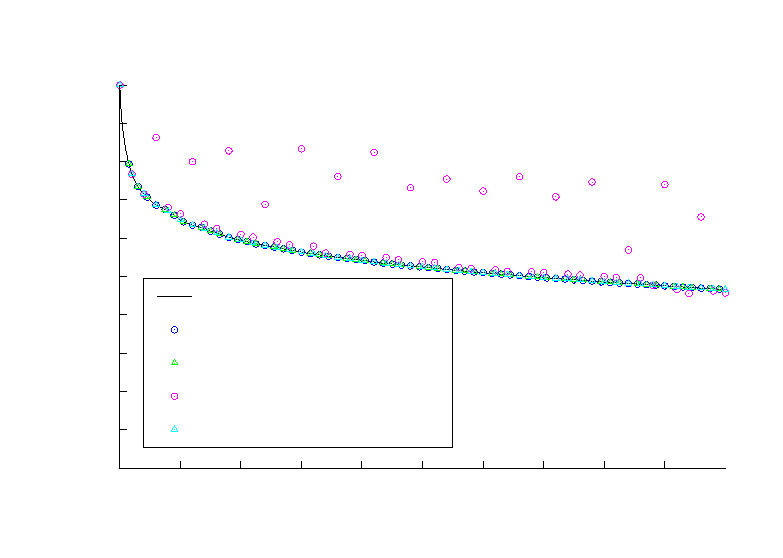
\includegraphics{dmat1}}%
    \gplfronttext
  \end{picture}%
\endgroup
}
	\caption{•••}
	\label{fig:dmat1}
\end{figure}
\begin{figure}
	\centering
	\resizebox{.9\textwidth}{!}{% GNUPLOT: LaTeX picture with Postscript
\begingroup
  \fontfamily{phv}%
  \selectfont
  \makeatletter
  \providecommand\color[2][]{%
    \GenericError{(gnuplot) \space\space\space\@spaces}{%
      Package color not loaded in conjunction with
      terminal option `colourtext'%
    }{See the gnuplot documentation for explanation.%
    }{Either use 'blacktext' in gnuplot or load the package
      color.sty in LaTeX.}%
    \renewcommand\color[2][]{}%
  }%
  \providecommand\includegraphics[2][]{%
    \GenericError{(gnuplot) \space\space\space\@spaces}{%
      Package graphicx or graphics not loaded%
    }{See the gnuplot documentation for explanation.%
    }{The gnuplot epslatex terminal needs graphicx.sty or graphics.sty.}%
    \renewcommand\includegraphics[2][]{}%
  }%
  \providecommand\rotatebox[2]{#2}%
  \@ifundefined{ifGPcolor}{%
    \newif\ifGPcolor
    \GPcolorfalse
  }{}%
  \@ifundefined{ifGPblacktext}{%
    \newif\ifGPblacktext
    \GPblacktexttrue
  }{}%
  % define a \g@addto@macro without @ in the name:
  \let\gplgaddtomacro\g@addto@macro
  % define empty templates for all commands taking text:
  \gdef\gplbacktext{}%
  \gdef\gplfronttext{}%
  \makeatother
  \ifGPblacktext
    % no textcolor at all
    \def\colorrgb#1{}%
    \def\colorgray#1{}%
  \else
    % gray or color?
    \ifGPcolor
      \def\colorrgb#1{\color[rgb]{#1}}%
      \def\colorgray#1{\color[gray]{#1}}%
      \expandafter\def\csname LTw\endcsname{\color{white}}%
      \expandafter\def\csname LTb\endcsname{\color{black}}%
      \expandafter\def\csname LTa\endcsname{\color{black}}%
      \expandafter\def\csname LT0\endcsname{\color[rgb]{1,0,0}}%
      \expandafter\def\csname LT1\endcsname{\color[rgb]{0,1,0}}%
      \expandafter\def\csname LT2\endcsname{\color[rgb]{0,0,1}}%
      \expandafter\def\csname LT3\endcsname{\color[rgb]{1,0,1}}%
      \expandafter\def\csname LT4\endcsname{\color[rgb]{0,1,1}}%
      \expandafter\def\csname LT5\endcsname{\color[rgb]{1,1,0}}%
      \expandafter\def\csname LT6\endcsname{\color[rgb]{0,0,0}}%
      \expandafter\def\csname LT7\endcsname{\color[rgb]{1,0.3,0}}%
      \expandafter\def\csname LT8\endcsname{\color[rgb]{0.5,0.5,0.5}}%
    \else
      % gray
      \def\colorrgb#1{\color{black}}%
      \def\colorgray#1{\color[gray]{#1}}%
      \expandafter\def\csname LTw\endcsname{\color{white}}%
      \expandafter\def\csname LTb\endcsname{\color{black}}%
      \expandafter\def\csname LTa\endcsname{\color{black}}%
      \expandafter\def\csname LT0\endcsname{\color{black}}%
      \expandafter\def\csname LT1\endcsname{\color{black}}%
      \expandafter\def\csname LT2\endcsname{\color{black}}%
      \expandafter\def\csname LT3\endcsname{\color{black}}%
      \expandafter\def\csname LT4\endcsname{\color{black}}%
      \expandafter\def\csname LT5\endcsname{\color{black}}%
      \expandafter\def\csname LT6\endcsname{\color{black}}%
      \expandafter\def\csname LT7\endcsname{\color{black}}%
      \expandafter\def\csname LT8\endcsname{\color{black}}%
    \fi
  \fi
    \setlength{\unitlength}{0.0500bp}%
    \ifx\gptboxheight\undefined%
      \newlength{\gptboxheight}%
      \newlength{\gptboxwidth}%
      \newsavebox{\gptboxtext}%
    \fi%
    \setlength{\fboxrule}{0.5pt}%
    \setlength{\fboxsep}{1pt}%
\begin{picture}(7200.00,5040.00)%
    \gplgaddtomacro\gplbacktext{%
      \csname LTb\endcsname%
      \put(858,704){\makebox(0,0)[r]{\strut{}\footnotesize -10}}%
      \put(858,1072){\makebox(0,0)[r]{\strut{}\footnotesize -9}}%
      \put(858,1439){\makebox(0,0)[r]{\strut{}\footnotesize -8}}%
      \put(858,1807){\makebox(0,0)[r]{\strut{}\footnotesize -7}}%
      \put(858,2174){\makebox(0,0)[r]{\strut{}\footnotesize -6}}%
      \put(858,2542){\makebox(0,0)[r]{\strut{}\footnotesize -5}}%
      \put(858,2909){\makebox(0,0)[r]{\strut{}\footnotesize -4}}%
      \put(858,3277){\makebox(0,0)[r]{\strut{}\footnotesize -3}}%
      \put(858,3644){\makebox(0,0)[r]{\strut{}\footnotesize -2}}%
      \put(858,4012){\makebox(0,0)[r]{\strut{}\footnotesize -1}}%
      \put(858,4379){\makebox(0,0)[r]{\strut{}\footnotesize 0}}%
      \put(1571,484){\makebox(0,0){\strut{}\footnotesize 100}}%
      \put(2153,484){\makebox(0,0){\strut{}\footnotesize 200}}%
      \put(2734,484){\makebox(0,0){\strut{}\footnotesize 300}}%
      \put(3315,484){\makebox(0,0){\strut{}\footnotesize 400}}%
      \put(3897,484){\makebox(0,0){\strut{}\footnotesize 500}}%
      \put(4478,484){\makebox(0,0){\strut{}\footnotesize 600}}%
      \put(5059,484){\makebox(0,0){\strut{}\footnotesize 700}}%
      \put(5640,484){\makebox(0,0){\strut{}\footnotesize 800}}%
      \put(6222,484){\makebox(0,0){\strut{}\footnotesize 900}}%
    }%
    \gplgaddtomacro\gplfronttext{%
      \csname LTb\endcsname%
      \put(352,2541){\rotatebox{-270}{\makebox(0,0){\strut{}\footnotesize Residual 2-norm, log scale}}}%
      \put(3896,154){\makebox(0,0){\strut{}\footnotesize Iteration count}}%
      \put(3896,4709){\makebox(0,0){\strut{}\shortstack{\footnotesize\,1e+04\,times,1e+04\,diagonal,\,logspace\,eigs,\,cond\,1e+10\\\footnotesize\,Residual\,2-norm,\,log\,scale}}}%
      \csname LTb\endcsname%
      \put(1800,2349){\makebox(0,0)[l]{\strut{}\scriptsize GMRES(120)}}%
      \csname LTb\endcsname%
      \put(1800,2030){\makebox(0,0)[l]{\strut{}\begin{minipage}[l]{.95\textwidth} \scriptsize Monomial-GMRES(15,8) \newline \tiny min, max rcond \#: 2.9e-12, 4.6e-12\end{minipage}}}%
      \csname LTb\endcsname%
      \put(1800,1711){\makebox(0,0)[l]{\strut{}\begin{minipage}[l]{.95\textwidth} \scriptsize Newton-GMRES(15,8) \newline \tiny min, max rcond \#: 2.6e-09, 3.4e-09\end{minipage}}}%
      \csname LTb\endcsname%
      \put(1800,1392){\makebox(0,0)[l]{\strut{}\begin{minipage}[l]{.95\textwidth} \scriptsize Monomial-GMRES(20,6) \newline \tiny min, max rcond \#: 3.7e-16, 6.6e-16\end{minipage}}}%
      \csname LTb\endcsname%
      \put(1800,1073){\makebox(0,0)[l]{\strut{}\begin{minipage}[l]{.95\textwidth} \scriptsize Newton-GMRES(20,6) \newline \tiny min, max rcond \#: 2.3e-12, 3.3e-12\end{minipage}}}%
    }%
    \gplbacktext
    \put(0,0){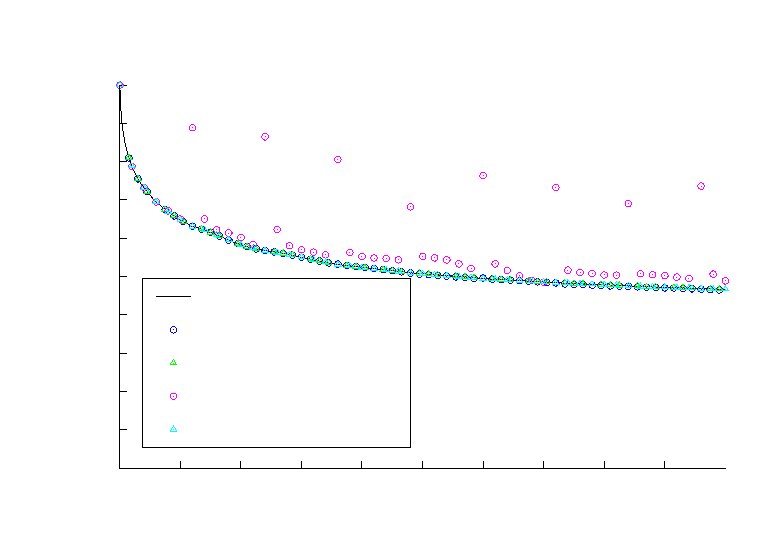
\includegraphics{dmat2}}%
    \gplfronttext
  \end{picture}%
\endgroup
}
	\caption{•••}
	\label{fig:dmat2}
\end{figure}
\begin{figure}
	\centering
	\resizebox{.9\textwidth}{!}{% GNUPLOT: LaTeX picture with Postscript
\begingroup
  \fontfamily{phv}%
  \selectfont
  \makeatletter
  \providecommand\color[2][]{%
    \GenericError{(gnuplot) \space\space\space\@spaces}{%
      Package color not loaded in conjunction with
      terminal option `colourtext'%
    }{See the gnuplot documentation for explanation.%
    }{Either use 'blacktext' in gnuplot or load the package
      color.sty in LaTeX.}%
    \renewcommand\color[2][]{}%
  }%
  \providecommand\includegraphics[2][]{%
    \GenericError{(gnuplot) \space\space\space\@spaces}{%
      Package graphicx or graphics not loaded%
    }{See the gnuplot documentation for explanation.%
    }{The gnuplot epslatex terminal needs graphicx.sty or graphics.sty.}%
    \renewcommand\includegraphics[2][]{}%
  }%
  \providecommand\rotatebox[2]{#2}%
  \@ifundefined{ifGPcolor}{%
    \newif\ifGPcolor
    \GPcolorfalse
  }{}%
  \@ifundefined{ifGPblacktext}{%
    \newif\ifGPblacktext
    \GPblacktexttrue
  }{}%
  % define a \g@addto@macro without @ in the name:
  \let\gplgaddtomacro\g@addto@macro
  % define empty templates for all commands taking text:
  \gdef\gplbacktext{}%
  \gdef\gplfronttext{}%
  \makeatother
  \ifGPblacktext
    % no textcolor at all
    \def\colorrgb#1{}%
    \def\colorgray#1{}%
  \else
    % gray or color?
    \ifGPcolor
      \def\colorrgb#1{\color[rgb]{#1}}%
      \def\colorgray#1{\color[gray]{#1}}%
      \expandafter\def\csname LTw\endcsname{\color{white}}%
      \expandafter\def\csname LTb\endcsname{\color{black}}%
      \expandafter\def\csname LTa\endcsname{\color{black}}%
      \expandafter\def\csname LT0\endcsname{\color[rgb]{1,0,0}}%
      \expandafter\def\csname LT1\endcsname{\color[rgb]{0,1,0}}%
      \expandafter\def\csname LT2\endcsname{\color[rgb]{0,0,1}}%
      \expandafter\def\csname LT3\endcsname{\color[rgb]{1,0,1}}%
      \expandafter\def\csname LT4\endcsname{\color[rgb]{0,1,1}}%
      \expandafter\def\csname LT5\endcsname{\color[rgb]{1,1,0}}%
      \expandafter\def\csname LT6\endcsname{\color[rgb]{0,0,0}}%
      \expandafter\def\csname LT7\endcsname{\color[rgb]{1,0.3,0}}%
      \expandafter\def\csname LT8\endcsname{\color[rgb]{0.5,0.5,0.5}}%
    \else
      % gray
      \def\colorrgb#1{\color{black}}%
      \def\colorgray#1{\color[gray]{#1}}%
      \expandafter\def\csname LTw\endcsname{\color{white}}%
      \expandafter\def\csname LTb\endcsname{\color{black}}%
      \expandafter\def\csname LTa\endcsname{\color{black}}%
      \expandafter\def\csname LT0\endcsname{\color{black}}%
      \expandafter\def\csname LT1\endcsname{\color{black}}%
      \expandafter\def\csname LT2\endcsname{\color{black}}%
      \expandafter\def\csname LT3\endcsname{\color{black}}%
      \expandafter\def\csname LT4\endcsname{\color{black}}%
      \expandafter\def\csname LT5\endcsname{\color{black}}%
      \expandafter\def\csname LT6\endcsname{\color{black}}%
      \expandafter\def\csname LT7\endcsname{\color{black}}%
      \expandafter\def\csname LT8\endcsname{\color{black}}%
    \fi
  \fi
    \setlength{\unitlength}{0.0500bp}%
    \ifx\gptboxheight\undefined%
      \newlength{\gptboxheight}%
      \newlength{\gptboxwidth}%
      \newsavebox{\gptboxtext}%
    \fi%
    \setlength{\fboxrule}{0.5pt}%
    \setlength{\fboxsep}{1pt}%
\begin{picture}(7200.00,5040.00)%
    \gplgaddtomacro\gplbacktext{%
      \csname LTb\endcsname%
      \put(858,704){\makebox(0,0)[r]{\strut{}\footnotesize -10}}%
      \put(858,1072){\makebox(0,0)[r]{\strut{}\footnotesize -9}}%
      \put(858,1439){\makebox(0,0)[r]{\strut{}\footnotesize -8}}%
      \put(858,1807){\makebox(0,0)[r]{\strut{}\footnotesize -7}}%
      \put(858,2174){\makebox(0,0)[r]{\strut{}\footnotesize -6}}%
      \put(858,2542){\makebox(0,0)[r]{\strut{}\footnotesize -5}}%
      \put(858,2909){\makebox(0,0)[r]{\strut{}\footnotesize -4}}%
      \put(858,3277){\makebox(0,0)[r]{\strut{}\footnotesize -3}}%
      \put(858,3644){\makebox(0,0)[r]{\strut{}\footnotesize -2}}%
      \put(858,4012){\makebox(0,0)[r]{\strut{}\footnotesize -1}}%
      \put(858,4379){\makebox(0,0)[r]{\strut{}\footnotesize 0}}%
      \put(1571,484){\makebox(0,0){\strut{}\footnotesize 100}}%
      \put(2153,484){\makebox(0,0){\strut{}\footnotesize 200}}%
      \put(2734,484){\makebox(0,0){\strut{}\footnotesize 300}}%
      \put(3315,484){\makebox(0,0){\strut{}\footnotesize 400}}%
      \put(3897,484){\makebox(0,0){\strut{}\footnotesize 500}}%
      \put(4478,484){\makebox(0,0){\strut{}\footnotesize 600}}%
      \put(5059,484){\makebox(0,0){\strut{}\footnotesize 700}}%
      \put(5640,484){\makebox(0,0){\strut{}\footnotesize 800}}%
      \put(6222,484){\makebox(0,0){\strut{}\footnotesize 900}}%
    }%
    \gplgaddtomacro\gplfronttext{%
      \csname LTb\endcsname%
      \put(352,2541){\rotatebox{-270}{\makebox(0,0){\strut{}\footnotesize Residual 2-norm, log scale}}}%
      \put(3896,154){\makebox(0,0){\strut{}\footnotesize Iteration count}}%
      \put(3896,4709){\makebox(0,0){\strut{}\shortstack{\footnotesize\,1e+04\,times,1e+04\,diagonal,\,logspace\,eigs,\,cond\,1e+15\\\footnotesize\,Residual\,2-norm,\,log\,scale}}}%
      \csname LTb\endcsname%
      \put(1800,2349){\makebox(0,0)[l]{\strut{}\scriptsize GMRES(120)}}%
      \csname LTb\endcsname%
      \put(1800,2030){\makebox(0,0)[l]{\strut{}\begin{minipage}[l]{.95\textwidth} \scriptsize Monomial-GMRES(15,8) \newline \tiny min, max rcond \#: 2.5e-12, 4.4e-12\end{minipage}}}%
      \csname LTb\endcsname%
      \put(1800,1711){\makebox(0,0)[l]{\strut{}\begin{minipage}[l]{.95\textwidth} \scriptsize Newton-GMRES(15,8) \newline \tiny min, max rcond \#: 1.7e-09, 3.5e-09\end{minipage}}}%
      \csname LTb\endcsname%
      \put(1800,1392){\makebox(0,0)[l]{\strut{}\begin{minipage}[l]{.95\textwidth} \scriptsize Monomial-GMRES(20,6) \newline \tiny min, max rcond \#: 2.9e-16, 7.6e-16\end{minipage}}}%
      \csname LTb\endcsname%
      \put(1800,1073){\makebox(0,0)[l]{\strut{}\begin{minipage}[l]{.95\textwidth} \scriptsize Newton-GMRES(20,6) \newline \tiny min, max rcond \#: 1.3e-12, 3.3e-12\end{minipage}}}%
    }%
    \gplbacktext
    \put(0,0){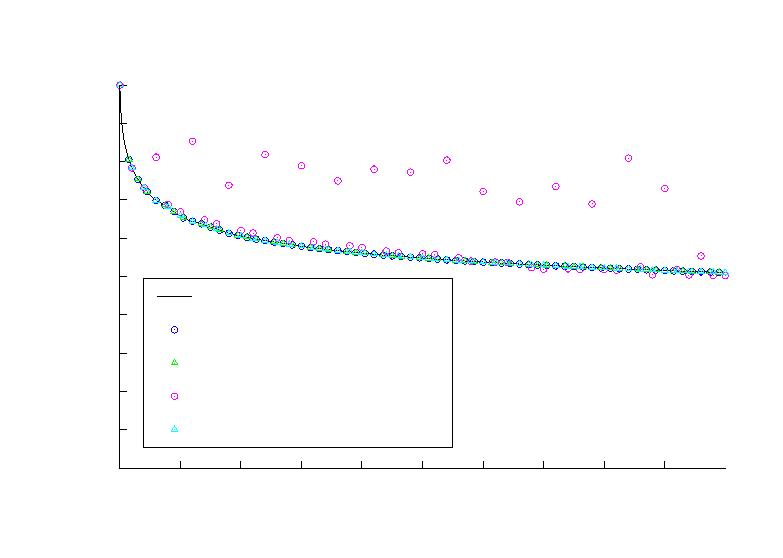
\includegraphics{dmat3}}%
    \gplfronttext
  \end{picture}%
\endgroup
}	
	\caption{•••}
	\label{fig:dmat3}
\end{figure}
\begin{figure}
	\centering
	\resizebox{.9\textwidth}{!}{% GNUPLOT: LaTeX picture with Postscript
\begingroup
  \fontfamily{phv}%
  \selectfont
  \makeatletter
  \providecommand\color[2][]{%
    \GenericError{(gnuplot) \space\space\space\@spaces}{%
      Package color not loaded in conjunction with
      terminal option `colourtext'%
    }{See the gnuplot documentation for explanation.%
    }{Either use 'blacktext' in gnuplot or load the package
      color.sty in LaTeX.}%
    \renewcommand\color[2][]{}%
  }%
  \providecommand\includegraphics[2][]{%
    \GenericError{(gnuplot) \space\space\space\@spaces}{%
      Package graphicx or graphics not loaded%
    }{See the gnuplot documentation for explanation.%
    }{The gnuplot epslatex terminal needs graphicx.sty or graphics.sty.}%
    \renewcommand\includegraphics[2][]{}%
  }%
  \providecommand\rotatebox[2]{#2}%
  \@ifundefined{ifGPcolor}{%
    \newif\ifGPcolor
    \GPcolorfalse
  }{}%
  \@ifundefined{ifGPblacktext}{%
    \newif\ifGPblacktext
    \GPblacktexttrue
  }{}%
  % define a \g@addto@macro without @ in the name:
  \let\gplgaddtomacro\g@addto@macro
  % define empty templates for all commands taking text:
  \gdef\gplbacktext{}%
  \gdef\gplfronttext{}%
  \makeatother
  \ifGPblacktext
    % no textcolor at all
    \def\colorrgb#1{}%
    \def\colorgray#1{}%
  \else
    % gray or color?
    \ifGPcolor
      \def\colorrgb#1{\color[rgb]{#1}}%
      \def\colorgray#1{\color[gray]{#1}}%
      \expandafter\def\csname LTw\endcsname{\color{white}}%
      \expandafter\def\csname LTb\endcsname{\color{black}}%
      \expandafter\def\csname LTa\endcsname{\color{black}}%
      \expandafter\def\csname LT0\endcsname{\color[rgb]{1,0,0}}%
      \expandafter\def\csname LT1\endcsname{\color[rgb]{0,1,0}}%
      \expandafter\def\csname LT2\endcsname{\color[rgb]{0,0,1}}%
      \expandafter\def\csname LT3\endcsname{\color[rgb]{1,0,1}}%
      \expandafter\def\csname LT4\endcsname{\color[rgb]{0,1,1}}%
      \expandafter\def\csname LT5\endcsname{\color[rgb]{1,1,0}}%
      \expandafter\def\csname LT6\endcsname{\color[rgb]{0,0,0}}%
      \expandafter\def\csname LT7\endcsname{\color[rgb]{1,0.3,0}}%
      \expandafter\def\csname LT8\endcsname{\color[rgb]{0.5,0.5,0.5}}%
    \else
      % gray
      \def\colorrgb#1{\color{black}}%
      \def\colorgray#1{\color[gray]{#1}}%
      \expandafter\def\csname LTw\endcsname{\color{white}}%
      \expandafter\def\csname LTb\endcsname{\color{black}}%
      \expandafter\def\csname LTa\endcsname{\color{black}}%
      \expandafter\def\csname LT0\endcsname{\color{black}}%
      \expandafter\def\csname LT1\endcsname{\color{black}}%
      \expandafter\def\csname LT2\endcsname{\color{black}}%
      \expandafter\def\csname LT3\endcsname{\color{black}}%
      \expandafter\def\csname LT4\endcsname{\color{black}}%
      \expandafter\def\csname LT5\endcsname{\color{black}}%
      \expandafter\def\csname LT6\endcsname{\color{black}}%
      \expandafter\def\csname LT7\endcsname{\color{black}}%
      \expandafter\def\csname LT8\endcsname{\color{black}}%
    \fi
  \fi
    \setlength{\unitlength}{0.0500bp}%
    \ifx\gptboxheight\undefined%
      \newlength{\gptboxheight}%
      \newlength{\gptboxwidth}%
      \newsavebox{\gptboxtext}%
    \fi%
    \setlength{\fboxrule}{0.5pt}%
    \setlength{\fboxsep}{1pt}%
\begin{picture}(7200.00,5040.00)%
    \gplgaddtomacro\gplbacktext{%
      \csname LTb\endcsname%
      \put(858,704){\makebox(0,0)[r]{\strut{}\footnotesize -10}}%
      \put(858,1072){\makebox(0,0)[r]{\strut{}\footnotesize -9}}%
      \put(858,1439){\makebox(0,0)[r]{\strut{}\footnotesize -8}}%
      \put(858,1807){\makebox(0,0)[r]{\strut{}\footnotesize -7}}%
      \put(858,2174){\makebox(0,0)[r]{\strut{}\footnotesize -6}}%
      \put(858,2542){\makebox(0,0)[r]{\strut{}\footnotesize -5}}%
      \put(858,2909){\makebox(0,0)[r]{\strut{}\footnotesize -4}}%
      \put(858,3277){\makebox(0,0)[r]{\strut{}\footnotesize -3}}%
      \put(858,3644){\makebox(0,0)[r]{\strut{}\footnotesize -2}}%
      \put(858,4012){\makebox(0,0)[r]{\strut{}\footnotesize -1}}%
      \put(858,4379){\makebox(0,0)[r]{\strut{}\footnotesize 0}}%
      \put(1571,484){\makebox(0,0){\strut{}\footnotesize 100}}%
      \put(2153,484){\makebox(0,0){\strut{}\footnotesize 200}}%
      \put(2734,484){\makebox(0,0){\strut{}\footnotesize 300}}%
      \put(3315,484){\makebox(0,0){\strut{}\footnotesize 400}}%
      \put(3897,484){\makebox(0,0){\strut{}\footnotesize 500}}%
      \put(4478,484){\makebox(0,0){\strut{}\footnotesize 600}}%
      \put(5059,484){\makebox(0,0){\strut{}\footnotesize 700}}%
      \put(5640,484){\makebox(0,0){\strut{}\footnotesize 800}}%
      \put(6222,484){\makebox(0,0){\strut{}\footnotesize 900}}%
			\put(6803,484){\makebox(0,0){\strut{}\footnotesize 1000}}%
    }%
    \gplgaddtomacro\gplfronttext{%
      \csname LTb\endcsname%
      \put(352,2541){\rotatebox{-270}{\makebox(0,0){\strut{}\footnotesize Residual 2-norm, log scale}}}%
      \put(3896,154){\makebox(0,0){\strut{}\footnotesize Iteration count}}%
      \put(3896,4709){\makebox(0,0){\strut{}\shortstack{\footnotesize\,1e+04\,times,1e+04\,diagonal,\,logspace\,eigs,\,cond\,1e+05\\\footnotesize\,Residual\,2-norm,\,log\,scale}}}%
      \csname LTb\endcsname%
      \put(1811,2349){\makebox(0,0)[l]{\strut{}\scriptsize GMRES(60)}}%
      \csname LTb\endcsname%
      \put(1811,2030){\makebox(0,0)[l]{\strut{}\begin{minipage}[l]{.95\textwidth} \scriptsize Monomial-GMRES(15,4) \newline \tiny min, max basis rcond \#: 4.67e-12, 5.19e-12\end{minipage}}}%
      \csname LTb\endcsname%
      \put(1811,1711){\makebox(0,0)[l]{\strut{}\begin{minipage}[l]{.95\textwidth} \scriptsize Newton-GMRES(15,4) \newline \tiny min, max basis rcond \#: 1.84e-02, 3.79e-02\end{minipage}}}%
      \csname LTb\endcsname%
      \put(1811,1392){\makebox(0,0)[l]{\strut{}\begin{minipage}[l]{.95\textwidth} \scriptsize Monomial-GMRES(20,3) \newline \tiny min, max basis rcond \#: 2.18e-16, 7.63e-16\end{minipage}}}%
      \csname LTb\endcsname%
      \put(1811,1073){\makebox(0,0)[l]{\strut{}\begin{minipage}[l]{.95\textwidth} \scriptsize Newton-GMRES(20,3) \newline \tiny min, max basis rcond \#: 8.62e-03, 1.38e-02\end{minipage}}}%
    }%
    \gplbacktext
    \put(0,0){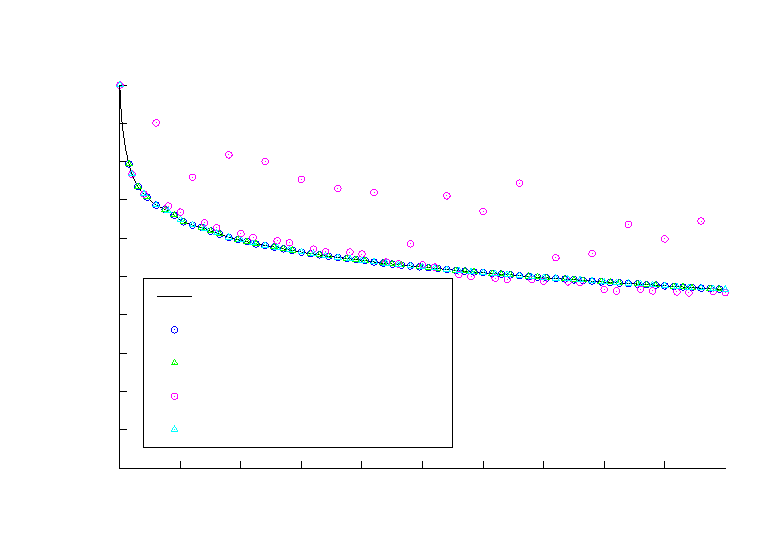
\includegraphics{dmat1_scale}}%
    \gplfronttext
  \end{picture}%
\endgroup
}
	\caption{•••}
	\label{fig:dmat1_scale}
\end{figure}
\begin{figure}
	\centering
	\resizebox{.9\textwidth}{!}{% GNUPLOT: LaTeX picture with Postscript
\begingroup
  \fontfamily{phv}%
  \selectfont
  \makeatletter
  \providecommand\color[2][]{%
    \GenericError{(gnuplot) \space\space\space\@spaces}{%
      Package color not loaded in conjunction with
      terminal option `colourtext'%
    }{See the gnuplot documentation for explanation.%
    }{Either use 'blacktext' in gnuplot or load the package
      color.sty in LaTeX.}%
    \renewcommand\color[2][]{}%
  }%
  \providecommand\includegraphics[2][]{%
    \GenericError{(gnuplot) \space\space\space\@spaces}{%
      Package graphicx or graphics not loaded%
    }{See the gnuplot documentation for explanation.%
    }{The gnuplot epslatex terminal needs graphicx.sty or graphics.sty.}%
    \renewcommand\includegraphics[2][]{}%
  }%
  \providecommand\rotatebox[2]{#2}%
  \@ifundefined{ifGPcolor}{%
    \newif\ifGPcolor
    \GPcolorfalse
  }{}%
  \@ifundefined{ifGPblacktext}{%
    \newif\ifGPblacktext
    \GPblacktexttrue
  }{}%
  % define a \g@addto@macro without @ in the name:
  \let\gplgaddtomacro\g@addto@macro
  % define empty templates for all commands taking text:
  \gdef\gplbacktext{}%
  \gdef\gplfronttext{}%
  \makeatother
  \ifGPblacktext
    % no textcolor at all
    \def\colorrgb#1{}%
    \def\colorgray#1{}%
  \else
    % gray or color?
    \ifGPcolor
      \def\colorrgb#1{\color[rgb]{#1}}%
      \def\colorgray#1{\color[gray]{#1}}%
      \expandafter\def\csname LTw\endcsname{\color{white}}%
      \expandafter\def\csname LTb\endcsname{\color{black}}%
      \expandafter\def\csname LTa\endcsname{\color{black}}%
      \expandafter\def\csname LT0\endcsname{\color[rgb]{1,0,0}}%
      \expandafter\def\csname LT1\endcsname{\color[rgb]{0,1,0}}%
      \expandafter\def\csname LT2\endcsname{\color[rgb]{0,0,1}}%
      \expandafter\def\csname LT3\endcsname{\color[rgb]{1,0,1}}%
      \expandafter\def\csname LT4\endcsname{\color[rgb]{0,1,1}}%
      \expandafter\def\csname LT5\endcsname{\color[rgb]{1,1,0}}%
      \expandafter\def\csname LT6\endcsname{\color[rgb]{0,0,0}}%
      \expandafter\def\csname LT7\endcsname{\color[rgb]{1,0.3,0}}%
      \expandafter\def\csname LT8\endcsname{\color[rgb]{0.5,0.5,0.5}}%
    \else
      % gray
      \def\colorrgb#1{\color{black}}%
      \def\colorgray#1{\color[gray]{#1}}%
      \expandafter\def\csname LTw\endcsname{\color{white}}%
      \expandafter\def\csname LTb\endcsname{\color{black}}%
      \expandafter\def\csname LTa\endcsname{\color{black}}%
      \expandafter\def\csname LT0\endcsname{\color{black}}%
      \expandafter\def\csname LT1\endcsname{\color{black}}%
      \expandafter\def\csname LT2\endcsname{\color{black}}%
      \expandafter\def\csname LT3\endcsname{\color{black}}%
      \expandafter\def\csname LT4\endcsname{\color{black}}%
      \expandafter\def\csname LT5\endcsname{\color{black}}%
      \expandafter\def\csname LT6\endcsname{\color{black}}%
      \expandafter\def\csname LT7\endcsname{\color{black}}%
      \expandafter\def\csname LT8\endcsname{\color{black}}%
    \fi
  \fi
    \setlength{\unitlength}{0.0500bp}%
    \ifx\gptboxheight\undefined%
      \newlength{\gptboxheight}%
      \newlength{\gptboxwidth}%
      \newsavebox{\gptboxtext}%
    \fi%
    \setlength{\fboxrule}{0.5pt}%
    \setlength{\fboxsep}{1pt}%
\begin{picture}(7200.00,5040.00)%
    \gplgaddtomacro\gplbacktext{%
      \csname LTb\endcsname%
      \put(858,704){\makebox(0,0)[r]{\strut{}\footnotesize -10}}%
      \put(858,1072){\makebox(0,0)[r]{\strut{}\footnotesize -9}}%
      \put(858,1439){\makebox(0,0)[r]{\strut{}\footnotesize -8}}%
      \put(858,1807){\makebox(0,0)[r]{\strut{}\footnotesize -7}}%
      \put(858,2174){\makebox(0,0)[r]{\strut{}\footnotesize -6}}%
      \put(858,2542){\makebox(0,0)[r]{\strut{}\footnotesize -5}}%
      \put(858,2909){\makebox(0,0)[r]{\strut{}\footnotesize -4}}%
      \put(858,3277){\makebox(0,0)[r]{\strut{}\footnotesize -3}}%
      \put(858,3644){\makebox(0,0)[r]{\strut{}\footnotesize -2}}%
      \put(858,4012){\makebox(0,0)[r]{\strut{}\footnotesize -1}}%
      \put(858,4379){\makebox(0,0)[r]{\strut{}\footnotesize 0}}%
      \put(1571,484){\makebox(0,0){\strut{}\footnotesize 100}}%
      \put(2153,484){\makebox(0,0){\strut{}\footnotesize 200}}%
      \put(2734,484){\makebox(0,0){\strut{}\footnotesize 300}}%
      \put(3315,484){\makebox(0,0){\strut{}\footnotesize 400}}%
      \put(3897,484){\makebox(0,0){\strut{}\footnotesize 500}}%
      \put(4478,484){\makebox(0,0){\strut{}\footnotesize 600}}%
      \put(5059,484){\makebox(0,0){\strut{}\footnotesize 700}}%
      \put(5640,484){\makebox(0,0){\strut{}\footnotesize 800}}%
      \put(6222,484){\makebox(0,0){\strut{}\footnotesize 900}}%
    }%
    \gplgaddtomacro\gplfronttext{%
      \csname LTb\endcsname%
      \put(352,2541){\rotatebox{-270}{\makebox(0,0){\strut{}\footnotesize Residual 2-norm, log scale}}}%
      \put(3896,154){\makebox(0,0){\strut{}\footnotesize Iteration count}}%
      \put(3896,4709){\makebox(0,0){\strut{}\shortstack{\footnotesize\,1e+04\,times,1e+04\,diagonal,\,logspace\,eigs,\,cond\,1e+10\\\footnotesize\,Residual\,2-norm,\,log\,scale}}}%
      \csname LTb\endcsname%
      \put(1811,2349){\makebox(0,0)[l]{\strut{}\scriptsize GMRES(60)}}%
      \csname LTb\endcsname%
      \put(1811,2030){\makebox(0,0)[l]{\strut{}\begin{minipage}[l]{.95\textwidth} \scriptsize Monomial-GMRES(15,4) \newline \tiny min, max basis rcond \#: 4.56e-12, 5.19e-12\end{minipage}}}%
      \csname LTb\endcsname%
      \put(1811,1711){\makebox(0,0)[l]{\strut{}\begin{minipage}[l]{.95\textwidth} \scriptsize Newton-GMRES(15,4) \newline \tiny min, max basis rcond \#: 1.74e-02, 3.50e-02\end{minipage}}}%
      \csname LTb\endcsname%
      \put(1811,1392){\makebox(0,0)[l]{\strut{}\begin{minipage}[l]{.95\textwidth} \scriptsize Monomial-GMRES(20,3) \newline \tiny min, max basis rcond \#: 2.39e-16, 6.93e-16\end{minipage}}}%
      \csname LTb\endcsname%
      \put(1811,1073){\makebox(0,0)[l]{\strut{}\begin{minipage}[l]{.95\textwidth} \scriptsize Newton-GMRES(20,3) \newline \tiny min, max basis rcond \#: 1.02e-02, 1.77e-02\end{minipage}}}%
    }%
    \gplbacktext
    \put(0,0){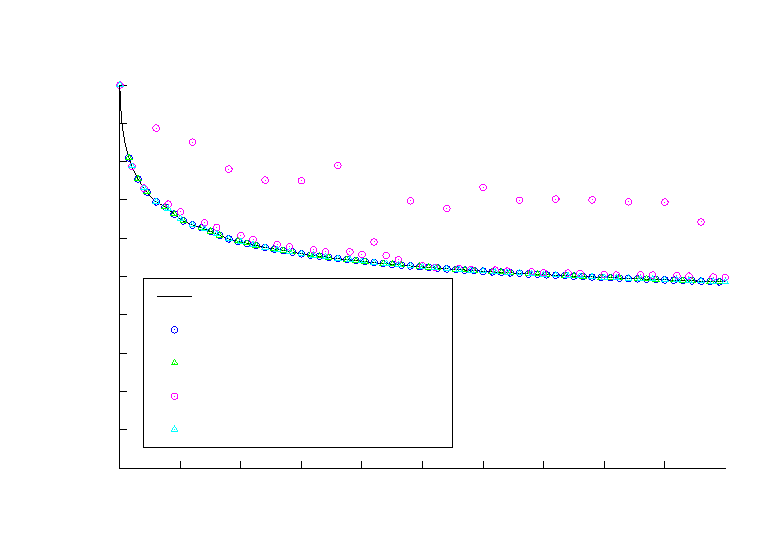
\includegraphics{dmat2_scale}}%
    \gplfronttext
  \end{picture}%
\endgroup
}
	\caption{•••}
	\label{fig:dmat2_scale}
\end{figure}
\begin{figure}
	\centering
	\resizebox{.9\textwidth}{!}{% GNUPLOT: LaTeX picture with Postscript
\begingroup
  \fontfamily{phv}%
  \selectfont
  \makeatletter
  \providecommand\color[2][]{%
    \GenericError{(gnuplot) \space\space\space\@spaces}{%
      Package color not loaded in conjunction with
      terminal option `colourtext'%
    }{See the gnuplot documentation for explanation.%
    }{Either use 'blacktext' in gnuplot or load the package
      color.sty in LaTeX.}%
    \renewcommand\color[2][]{}%
  }%
  \providecommand\includegraphics[2][]{%
    \GenericError{(gnuplot) \space\space\space\@spaces}{%
      Package graphicx or graphics not loaded%
    }{See the gnuplot documentation for explanation.%
    }{The gnuplot epslatex terminal needs graphicx.sty or graphics.sty.}%
    \renewcommand\includegraphics[2][]{}%
  }%
  \providecommand\rotatebox[2]{#2}%
  \@ifundefined{ifGPcolor}{%
    \newif\ifGPcolor
    \GPcolorfalse
  }{}%
  \@ifundefined{ifGPblacktext}{%
    \newif\ifGPblacktext
    \GPblacktexttrue
  }{}%
  % define a \g@addto@macro without @ in the name:
  \let\gplgaddtomacro\g@addto@macro
  % define empty templates for all commands taking text:
  \gdef\gplbacktext{}%
  \gdef\gplfronttext{}%
  \makeatother
  \ifGPblacktext
    % no textcolor at all
    \def\colorrgb#1{}%
    \def\colorgray#1{}%
  \else
    % gray or color?
    \ifGPcolor
      \def\colorrgb#1{\color[rgb]{#1}}%
      \def\colorgray#1{\color[gray]{#1}}%
      \expandafter\def\csname LTw\endcsname{\color{white}}%
      \expandafter\def\csname LTb\endcsname{\color{black}}%
      \expandafter\def\csname LTa\endcsname{\color{black}}%
      \expandafter\def\csname LT0\endcsname{\color[rgb]{1,0,0}}%
      \expandafter\def\csname LT1\endcsname{\color[rgb]{0,1,0}}%
      \expandafter\def\csname LT2\endcsname{\color[rgb]{0,0,1}}%
      \expandafter\def\csname LT3\endcsname{\color[rgb]{1,0,1}}%
      \expandafter\def\csname LT4\endcsname{\color[rgb]{0,1,1}}%
      \expandafter\def\csname LT5\endcsname{\color[rgb]{1,1,0}}%
      \expandafter\def\csname LT6\endcsname{\color[rgb]{0,0,0}}%
      \expandafter\def\csname LT7\endcsname{\color[rgb]{1,0.3,0}}%
      \expandafter\def\csname LT8\endcsname{\color[rgb]{0.5,0.5,0.5}}%
    \else
      % gray
      \def\colorrgb#1{\color{black}}%
      \def\colorgray#1{\color[gray]{#1}}%
      \expandafter\def\csname LTw\endcsname{\color{white}}%
      \expandafter\def\csname LTb\endcsname{\color{black}}%
      \expandafter\def\csname LTa\endcsname{\color{black}}%
      \expandafter\def\csname LT0\endcsname{\color{black}}%
      \expandafter\def\csname LT1\endcsname{\color{black}}%
      \expandafter\def\csname LT2\endcsname{\color{black}}%
      \expandafter\def\csname LT3\endcsname{\color{black}}%
      \expandafter\def\csname LT4\endcsname{\color{black}}%
      \expandafter\def\csname LT5\endcsname{\color{black}}%
      \expandafter\def\csname LT6\endcsname{\color{black}}%
      \expandafter\def\csname LT7\endcsname{\color{black}}%
      \expandafter\def\csname LT8\endcsname{\color{black}}%
    \fi
  \fi
    \setlength{\unitlength}{0.0500bp}%
    \ifx\gptboxheight\undefined%
      \newlength{\gptboxheight}%
      \newlength{\gptboxwidth}%
      \newsavebox{\gptboxtext}%
    \fi%
    \setlength{\fboxrule}{0.5pt}%
    \setlength{\fboxsep}{1pt}%
\begin{picture}(7200.00,5040.00)%
    \gplgaddtomacro\gplbacktext{%
      \csname LTb\endcsname%
      \put(858,704){\makebox(0,0)[r]{\strut{}\footnotesize -10}}%
      \put(858,1072){\makebox(0,0)[r]{\strut{}\footnotesize -9}}%
      \put(858,1439){\makebox(0,0)[r]{\strut{}\footnotesize -8}}%
      \put(858,1807){\makebox(0,0)[r]{\strut{}\footnotesize -7}}%
      \put(858,2174){\makebox(0,0)[r]{\strut{}\footnotesize -6}}%
      \put(858,2542){\makebox(0,0)[r]{\strut{}\footnotesize -5}}%
      \put(858,2909){\makebox(0,0)[r]{\strut{}\footnotesize -4}}%
      \put(858,3277){\makebox(0,0)[r]{\strut{}\footnotesize -3}}%
      \put(858,3644){\makebox(0,0)[r]{\strut{}\footnotesize -2}}%
      \put(858,4012){\makebox(0,0)[r]{\strut{}\footnotesize -1}}%
      \put(858,4379){\makebox(0,0)[r]{\strut{}\footnotesize 0}}%
      \put(1571,484){\makebox(0,0){\strut{}\footnotesize 100}}%
      \put(2153,484){\makebox(0,0){\strut{}\footnotesize 200}}%
      \put(2734,484){\makebox(0,0){\strut{}\footnotesize 300}}%
      \put(3315,484){\makebox(0,0){\strut{}\footnotesize 400}}%
      \put(3897,484){\makebox(0,0){\strut{}\footnotesize 500}}%
      \put(4478,484){\makebox(0,0){\strut{}\footnotesize 600}}%
      \put(5059,484){\makebox(0,0){\strut{}\footnotesize 700}}%
      \put(5640,484){\makebox(0,0){\strut{}\footnotesize 800}}%
      \put(6222,484){\makebox(0,0){\strut{}\footnotesize 900}}%
			\put(6803,484){\makebox(0,0){\strut{}\footnotesize 1000}}%
    }%
    \gplgaddtomacro\gplfronttext{%
      \csname LTb\endcsname%
      \put(352,2541){\rotatebox{-270}{\makebox(0,0){\strut{}\footnotesize Residual 2-norm, log scale}}}%
      \put(3896,154){\makebox(0,0){\strut{}\footnotesize Iteration count}}%
      \put(3896,4709){\makebox(0,0){\strut{}\shortstack{\footnotesize\,1e+04\,times,1e+04\,diagonal,\,logspace\,eigs,\,cond\,1e+15\\\footnotesize\,Residual\,2-norm,\,log\,scale}}}%
      \csname LTb\endcsname%
      \put(1811,2349){\makebox(0,0)[l]{\strut{}\scriptsize GMRES(60)}}%
      \csname LTb\endcsname%
      \put(1811,2030){\makebox(0,0)[l]{\strut{}\begin{minipage}[l]{.95\textwidth} \scriptsize Monomial-GMRES(15,4) \newline \tiny min, max basis rcond \#: 4.39e-12, 5.34e-12\end{minipage}}}%
      \csname LTb\endcsname%
      \put(1811,1711){\makebox(0,0)[l]{\strut{}\begin{minipage}[l]{.95\textwidth} \scriptsize Newton-GMRES(15,4) \newline \tiny min, max basis rcond \#: 1.66e-02, 3.93e-02\end{minipage}}}%
      \csname LTb\endcsname%
      \put(1811,1392){\makebox(0,0)[l]{\strut{}\begin{minipage}[l]{.95\textwidth} \scriptsize Monomial-GMRES(20,3) \newline \tiny min, max basis rcond \#: 1.24e-16, 6.65e-16\end{minipage}}}%
      \csname LTb\endcsname%
      \put(1811,1073){\makebox(0,0)[l]{\strut{}\begin{minipage}[l]{.95\textwidth} \scriptsize Newton-GMRES(20,3) \newline \tiny min, max basis rcond \#: 1.01e-02, 1.58e-02\end{minipage}}}%
    }%
    \gplbacktext
    \put(0,0){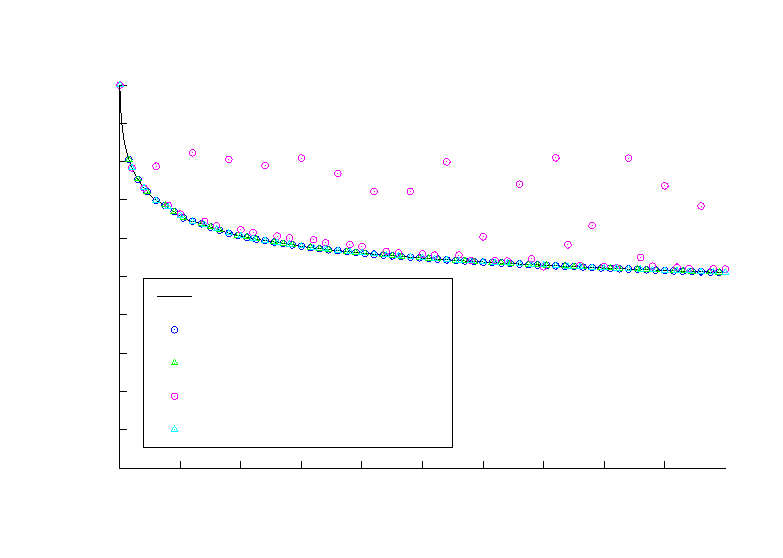
\includegraphics{dmat3_scale}}%
    \gplfronttext
  \end{picture}%
\endgroup
}
	\caption{•••}
	\label{fig:dmat3_scale}
\end{figure}
\begin{figure}
	\centering
	\resizebox{.9\textwidth}{!}{% GNUPLOT: LaTeX picture with Postscript
\begingroup
  \fontfamily{phv}%
  \selectfont
  \makeatletter
  \providecommand\color[2][]{%
    \GenericError{(gnuplot) \space\space\space\@spaces}{%
      Package color not loaded in conjunction with
      terminal option `colourtext'%
    }{See the gnuplot documentation for explanation.%
    }{Either use 'blacktext' in gnuplot or load the package
      color.sty in LaTeX.}%
    \renewcommand\color[2][]{}%
  }%
  \providecommand\includegraphics[2][]{%
    \GenericError{(gnuplot) \space\space\space\@spaces}{%
      Package graphicx or graphics not loaded%
    }{See the gnuplot documentation for explanation.%
    }{The gnuplot epslatex terminal needs graphicx.sty or graphics.sty.}%
    \renewcommand\includegraphics[2][]{}%
  }%
  \providecommand\rotatebox[2]{#2}%
  \@ifundefined{ifGPcolor}{%
    \newif\ifGPcolor
    \GPcolorfalse
  }{}%
  \@ifundefined{ifGPblacktext}{%
    \newif\ifGPblacktext
    \GPblacktexttrue
  }{}%
  % define a \g@addto@macro without @ in the name:
  \let\gplgaddtomacro\g@addto@macro
  % define empty templates for all commands taking text:
  \gdef\gplbacktext{}%
  \gdef\gplfronttext{}%
  \makeatother
  \ifGPblacktext
    % no textcolor at all
    \def\colorrgb#1{}%
    \def\colorgray#1{}%
  \else
    % gray or color?
    \ifGPcolor
      \def\colorrgb#1{\color[rgb]{#1}}%
      \def\colorgray#1{\color[gray]{#1}}%
      \expandafter\def\csname LTw\endcsname{\color{white}}%
      \expandafter\def\csname LTb\endcsname{\color{black}}%
      \expandafter\def\csname LTa\endcsname{\color{black}}%
      \expandafter\def\csname LT0\endcsname{\color[rgb]{1,0,0}}%
      \expandafter\def\csname LT1\endcsname{\color[rgb]{0,1,0}}%
      \expandafter\def\csname LT2\endcsname{\color[rgb]{0,0,1}}%
      \expandafter\def\csname LT3\endcsname{\color[rgb]{1,0,1}}%
      \expandafter\def\csname LT4\endcsname{\color[rgb]{0,1,1}}%
      \expandafter\def\csname LT5\endcsname{\color[rgb]{1,1,0}}%
      \expandafter\def\csname LT6\endcsname{\color[rgb]{0,0,0}}%
      \expandafter\def\csname LT7\endcsname{\color[rgb]{1,0.3,0}}%
      \expandafter\def\csname LT8\endcsname{\color[rgb]{0.5,0.5,0.5}}%
    \else
      % gray
      \def\colorrgb#1{\color{black}}%
      \def\colorgray#1{\color[gray]{#1}}%
      \expandafter\def\csname LTw\endcsname{\color{white}}%
      \expandafter\def\csname LTb\endcsname{\color{black}}%
      \expandafter\def\csname LTa\endcsname{\color{black}}%
      \expandafter\def\csname LT0\endcsname{\color{black}}%
      \expandafter\def\csname LT1\endcsname{\color{black}}%
      \expandafter\def\csname LT2\endcsname{\color{black}}%
      \expandafter\def\csname LT3\endcsname{\color{black}}%
      \expandafter\def\csname LT4\endcsname{\color{black}}%
      \expandafter\def\csname LT5\endcsname{\color{black}}%
      \expandafter\def\csname LT6\endcsname{\color{black}}%
      \expandafter\def\csname LT7\endcsname{\color{black}}%
      \expandafter\def\csname LT8\endcsname{\color{black}}%
    \fi
  \fi
    \setlength{\unitlength}{0.0500bp}%
    \ifx\gptboxheight\undefined%
      \newlength{\gptboxheight}%
      \newlength{\gptboxwidth}%
      \newsavebox{\gptboxtext}%
    \fi%
    \setlength{\fboxrule}{0.5pt}%
    \setlength{\fboxsep}{1pt}%
\begin{picture}(7200.00,5040.00)%
    \gplgaddtomacro\gplbacktext{%
      \csname LTb\endcsname%
      \put(858,704){\makebox(0,0)[r]{\strut{}\footnotesize -16}}%
      \put(858,1163){\makebox(0,0)[r]{\strut{}\footnotesize -14}}%
      \put(858,1623){\makebox(0,0)[r]{\strut{}\footnotesize -12}}%
      \put(858,2082){\makebox(0,0)[r]{\strut{}\footnotesize -10}}%
      \put(858,2542){\makebox(0,0)[r]{\strut{}\footnotesize -8}}%
      \put(858,3001){\makebox(0,0)[r]{\strut{}\footnotesize -6}}%
      \put(858,3460){\makebox(0,0)[r]{\strut{}\footnotesize -4}}%
      \put(858,3920){\makebox(0,0)[r]{\strut{}\footnotesize -2}}%
      \put(858,4379){\makebox(0,0)[r]{\strut{}\footnotesize 0}}%
      \put(1571,484){\makebox(0,0){\strut{}\footnotesize 100}}%
      \put(2153,484){\makebox(0,0){\strut{}\footnotesize 200}}%
      \put(2734,484){\makebox(0,0){\strut{}\footnotesize 300}}%
      \put(3315,484){\makebox(0,0){\strut{}\footnotesize 400}}%
      \put(3897,484){\makebox(0,0){\strut{}\footnotesize 500}}%
      \put(4478,484){\makebox(0,0){\strut{}\footnotesize 600}}%
      \put(5059,484){\makebox(0,0){\strut{}\footnotesize 700}}%
      \put(5640,484){\makebox(0,0){\strut{}\footnotesize 800}}%
      \put(6222,484){\makebox(0,0){\strut{}\footnotesize 900}}%
			\put(6803,484){\makebox(0,0){\strut{}\footnotesize 1000}}%
    }%
    \gplgaddtomacro\gplfronttext{%
      \csname LTb\endcsname%
      \put(352,2541){\rotatebox{-270}{\makebox(0,0){\strut{}\footnotesize Residual 2-norm, log scale}}}%
      \put(3896,154){\makebox(0,0){\strut{}\footnotesize Iteration count}}%
      \put(3896,4709){\makebox(0,0){\strut{}\shortstack{Watt1}}}%
      \csname LTb\endcsname%
      \put(4311,4192){\makebox(0,0)[l]{\strut{}\scriptsize GMRES(30)}}%
      \csname LTb\endcsname%
      \put(4311,3873){\makebox(0,0)[l]{\strut{}\begin{minipage}[l]{.95\textwidth} \scriptsize Monomial-GMRES(3,10) \newline \tiny min, max basis rcond \#: 9.80e-15, 2.99e-08\end{minipage}}}%
      \csname LTb\endcsname%
      \put(4311,3554){\makebox(0,0)[l]{\strut{}\begin{minipage}[l]{.95\textwidth} \scriptsize Newton-GMRES(3,10) \newline \tiny min, max basis rcond \#: 1.05e-13, 2.11e-07\end{minipage}}}%
      \csname LTb\endcsname%
      \put(4311,3235){\makebox(0,0)[l]{\strut{}\begin{minipage}[l]{.95\textwidth} \scriptsize Monomial-GMRES(5,6) \newline \tiny min, max basis rcond \#: 2.94e-17, 8.57e-11\end{minipage}}}%
      \csname LTb\endcsname%
      \put(4311,2916){\makebox(0,0)[l]{\strut{}\begin{minipage}[l]{.95\textwidth} \scriptsize Newton-GMRES(5,6) \newline \tiny min, max basis rcond \#: 2.71e-25, 4.17e-14\end{minipage}}}%
    }%
    \gplbacktext
    \put(0,0){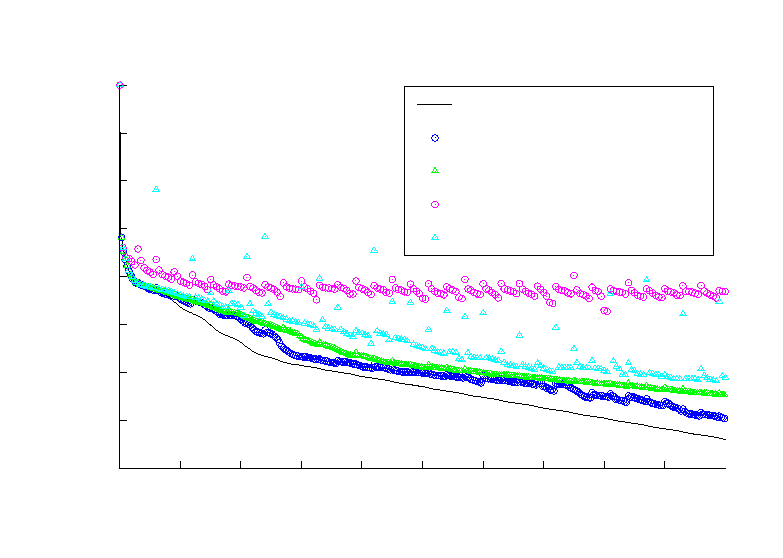
\includegraphics{watt1_noscale}}%
    \gplfronttext
  \end{picture}%
\endgroup
}
	\caption{not scaled}
	\label{fig:watt1_noscale}
\end{figure}
\begin{figure}
	\centering
	\resizebox{.9\textwidth}{!}{% GNUPLOT: LaTeX picture with Postscript
\begingroup
  \fontfamily{phv}%
  \selectfont
  \makeatletter
  \providecommand\color[2][]{%
    \GenericError{(gnuplot) \space\space\space\@spaces}{%
      Package color not loaded in conjunction with
      terminal option `colourtext'%
    }{See the gnuplot documentation for explanation.%
    }{Either use 'blacktext' in gnuplot or load the package
      color.sty in LaTeX.}%
    \renewcommand\color[2][]{}%
  }%
  \providecommand\includegraphics[2][]{%
    \GenericError{(gnuplot) \space\space\space\@spaces}{%
      Package graphicx or graphics not loaded%
    }{See the gnuplot documentation for explanation.%
    }{The gnuplot epslatex terminal needs graphicx.sty or graphics.sty.}%
    \renewcommand\includegraphics[2][]{}%
  }%
  \providecommand\rotatebox[2]{#2}%
  \@ifundefined{ifGPcolor}{%
    \newif\ifGPcolor
    \GPcolorfalse
  }{}%
  \@ifundefined{ifGPblacktext}{%
    \newif\ifGPblacktext
    \GPblacktexttrue
  }{}%
  % define a \g@addto@macro without @ in the name:
  \let\gplgaddtomacro\g@addto@macro
  % define empty templates for all commands taking text:
  \gdef\gplbacktext{}%
  \gdef\gplfronttext{}%
  \makeatother
  \ifGPblacktext
    % no textcolor at all
    \def\colorrgb#1{}%
    \def\colorgray#1{}%
  \else
    % gray or color?
    \ifGPcolor
      \def\colorrgb#1{\color[rgb]{#1}}%
      \def\colorgray#1{\color[gray]{#1}}%
      \expandafter\def\csname LTw\endcsname{\color{white}}%
      \expandafter\def\csname LTb\endcsname{\color{black}}%
      \expandafter\def\csname LTa\endcsname{\color{black}}%
      \expandafter\def\csname LT0\endcsname{\color[rgb]{1,0,0}}%
      \expandafter\def\csname LT1\endcsname{\color[rgb]{0,1,0}}%
      \expandafter\def\csname LT2\endcsname{\color[rgb]{0,0,1}}%
      \expandafter\def\csname LT3\endcsname{\color[rgb]{1,0,1}}%
      \expandafter\def\csname LT4\endcsname{\color[rgb]{0,1,1}}%
      \expandafter\def\csname LT5\endcsname{\color[rgb]{1,1,0}}%
      \expandafter\def\csname LT6\endcsname{\color[rgb]{0,0,0}}%
      \expandafter\def\csname LT7\endcsname{\color[rgb]{1,0.3,0}}%
      \expandafter\def\csname LT8\endcsname{\color[rgb]{0.5,0.5,0.5}}%
    \else
      % gray
      \def\colorrgb#1{\color{black}}%
      \def\colorgray#1{\color[gray]{#1}}%
      \expandafter\def\csname LTw\endcsname{\color{white}}%
      \expandafter\def\csname LTb\endcsname{\color{black}}%
      \expandafter\def\csname LTa\endcsname{\color{black}}%
      \expandafter\def\csname LT0\endcsname{\color{black}}%
      \expandafter\def\csname LT1\endcsname{\color{black}}%
      \expandafter\def\csname LT2\endcsname{\color{black}}%
      \expandafter\def\csname LT3\endcsname{\color{black}}%
      \expandafter\def\csname LT4\endcsname{\color{black}}%
      \expandafter\def\csname LT5\endcsname{\color{black}}%
      \expandafter\def\csname LT6\endcsname{\color{black}}%
      \expandafter\def\csname LT7\endcsname{\color{black}}%
      \expandafter\def\csname LT8\endcsname{\color{black}}%
    \fi
  \fi
    \setlength{\unitlength}{0.0500bp}%
    \ifx\gptboxheight\undefined%
      \newlength{\gptboxheight}%
      \newlength{\gptboxwidth}%
      \newsavebox{\gptboxtext}%
    \fi%
    \setlength{\fboxrule}{0.5pt}%
    \setlength{\fboxsep}{1pt}%
\begin{picture}(7200.00,5040.00)%
    \gplgaddtomacro\gplbacktext{%
      \csname LTb\endcsname%
      \put(858,704){\makebox(0,0)[r]{\strut{}\footnotesize -16}}%
      \put(858,1163){\makebox(0,0)[r]{\strut{}\footnotesize -14}}%
      \put(858,1623){\makebox(0,0)[r]{\strut{}\footnotesize -12}}%
      \put(858,2082){\makebox(0,0)[r]{\strut{}\footnotesize -10}}%
      \put(858,2542){\makebox(0,0)[r]{\strut{}\footnotesize -8}}%
      \put(858,3001){\makebox(0,0)[r]{\strut{}\footnotesize -6}}%
      \put(858,3460){\makebox(0,0)[r]{\strut{}\footnotesize -4}}%
      \put(858,3920){\makebox(0,0)[r]{\strut{}\footnotesize -2}}%
      \put(858,4379){\makebox(0,0)[r]{\strut{}\footnotesize 0}}%
      \put(1571,484){\makebox(0,0){\strut{}\footnotesize 100}}%
      \put(2153,484){\makebox(0,0){\strut{}\footnotesize 200}}%
      \put(2734,484){\makebox(0,0){\strut{}\footnotesize 300}}%
      \put(3315,484){\makebox(0,0){\strut{}\footnotesize 400}}%
      \put(3897,484){\makebox(0,0){\strut{}\footnotesize 500}}%
      \put(4478,484){\makebox(0,0){\strut{}\footnotesize 600}}%
      \put(5059,484){\makebox(0,0){\strut{}\footnotesize 700}}%
      \put(5640,484){\makebox(0,0){\strut{}\footnotesize 800}}%
      \put(6222,484){\makebox(0,0){\strut{}\footnotesize 900}}%
			\put(6803,484){\makebox(0,0){\strut{}\footnotesize 1000}}%
    }%
    \gplgaddtomacro\gplfronttext{%
      \csname LTb\endcsname%
      \put(352,2541){\rotatebox{-270}{\makebox(0,0){\strut{}\footnotesize Residual 2-norm, log scale}}}%
      \put(3896,154){\makebox(0,0){\strut{}\footnotesize Iteration count}}%
      \put(3896,4709){\makebox(0,0){\strut{}\shortstack{Watt1}}}%
      \csname LTb\endcsname%
      \put(4311,4192){\makebox(0,0)[l]{\strut{}\scriptsize GMRES(30)}}%
      \csname LTb\endcsname%
      \put(4311,3873){\makebox(0,0)[l]{\strut{}\begin{minipage}[l]{.95\textwidth} \scriptsize Monomial-GMRES(5,6) \newline \tiny min, max basis rcond \#: 3.62e-17, 6.40e-11\end{minipage}}}%
      \csname LTb\endcsname%
      \put(4311,3554){\makebox(0,0)[l]{\strut{}\begin{minipage}[l]{.95\textwidth} \scriptsize Newton-GMRES(5,6) \newline \tiny min, max basis rcond \#: 1.15e-16, 1.44e-01\end{minipage}}}%
      \csname LTb\endcsname%
      \put(4311,3235){\makebox(0,0)[l]{\strut{}\begin{minipage}[l]{.95\textwidth} \scriptsize Monomial-GMRES(6,5) \newline \tiny min, max basis rcond \#: 2.41e-17, 3.54e-11\end{minipage}}}%
      \csname LTb\endcsname%
      \put(4311,2916){\makebox(0,0)[l]{\strut{}\begin{minipage}[l]{.95\textwidth} \scriptsize Newton-GMRES(6,5) \newline \tiny min, max basis rcond \#: 1.19e-14, 1.61e-02\end{minipage}}}%
    }%
    \gplbacktext
    \put(0,0){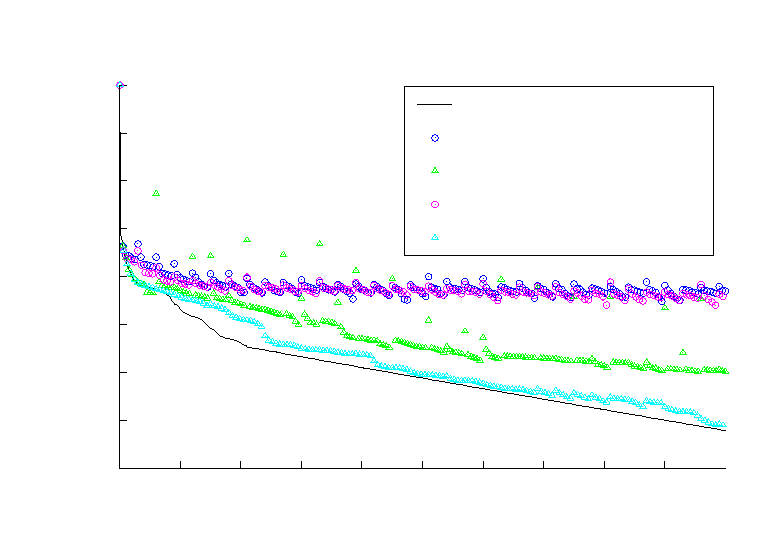
\includegraphics{watt1_scale}}%
    \gplfronttext
  \end{picture}%
\endgroup
}
	\caption{•••}
	\label{fig:watt1_scale}
\end{figure}
\begin{figure}
	\centering
	\resizebox{.9\textwidth}{!}{% GNUPLOT: LaTeX picture with Postscript
\begingroup
  \fontfamily{phv}%
  \selectfont
  \makeatletter
  \providecommand\color[2][]{%
    \GenericError{(gnuplot) \space\space\space\@spaces}{%
      Package color not loaded in conjunction with
      terminal option `colourtext'%
    }{See the gnuplot documentation for explanation.%
    }{Either use 'blacktext' in gnuplot or load the package
      color.sty in LaTeX.}%
    \renewcommand\color[2][]{}%
  }%
  \providecommand\includegraphics[2][]{%
    \GenericError{(gnuplot) \space\space\space\@spaces}{%
      Package graphicx or graphics not loaded%
    }{See the gnuplot documentation for explanation.%
    }{The gnuplot epslatex terminal needs graphicx.sty or graphics.sty.}%
    \renewcommand\includegraphics[2][]{}%
  }%
  \providecommand\rotatebox[2]{#2}%
  \@ifundefined{ifGPcolor}{%
    \newif\ifGPcolor
    \GPcolorfalse
  }{}%
  \@ifundefined{ifGPblacktext}{%
    \newif\ifGPblacktext
    \GPblacktexttrue
  }{}%
  % define a \g@addto@macro without @ in the name:
  \let\gplgaddtomacro\g@addto@macro
  % define empty templates for all commands taking text:
  \gdef\gplbacktext{}%
  \gdef\gplfronttext{}%
  \makeatother
  \ifGPblacktext
    % no textcolor at all
    \def\colorrgb#1{}%
    \def\colorgray#1{}%
  \else
    % gray or color?
    \ifGPcolor
      \def\colorrgb#1{\color[rgb]{#1}}%
      \def\colorgray#1{\color[gray]{#1}}%
      \expandafter\def\csname LTw\endcsname{\color{white}}%
      \expandafter\def\csname LTb\endcsname{\color{black}}%
      \expandafter\def\csname LTa\endcsname{\color{black}}%
      \expandafter\def\csname LT0\endcsname{\color[rgb]{1,0,0}}%
      \expandafter\def\csname LT1\endcsname{\color[rgb]{0,1,0}}%
      \expandafter\def\csname LT2\endcsname{\color[rgb]{0,0,1}}%
      \expandafter\def\csname LT3\endcsname{\color[rgb]{1,0,1}}%
      \expandafter\def\csname LT4\endcsname{\color[rgb]{0,1,1}}%
      \expandafter\def\csname LT5\endcsname{\color[rgb]{1,1,0}}%
      \expandafter\def\csname LT6\endcsname{\color[rgb]{0,0,0}}%
      \expandafter\def\csname LT7\endcsname{\color[rgb]{1,0.3,0}}%
      \expandafter\def\csname LT8\endcsname{\color[rgb]{0.5,0.5,0.5}}%
    \else
      % gray
      \def\colorrgb#1{\color{black}}%
      \def\colorgray#1{\color[gray]{#1}}%
      \expandafter\def\csname LTw\endcsname{\color{white}}%
      \expandafter\def\csname LTb\endcsname{\color{black}}%
      \expandafter\def\csname LTa\endcsname{\color{black}}%
      \expandafter\def\csname LT0\endcsname{\color{black}}%
      \expandafter\def\csname LT1\endcsname{\color{black}}%
      \expandafter\def\csname LT2\endcsname{\color{black}}%
      \expandafter\def\csname LT3\endcsname{\color{black}}%
      \expandafter\def\csname LT4\endcsname{\color{black}}%
      \expandafter\def\csname LT5\endcsname{\color{black}}%
      \expandafter\def\csname LT6\endcsname{\color{black}}%
      \expandafter\def\csname LT7\endcsname{\color{black}}%
      \expandafter\def\csname LT8\endcsname{\color{black}}%
    \fi
  \fi
    \setlength{\unitlength}{0.0500bp}%
    \ifx\gptboxheight\undefined%
      \newlength{\gptboxheight}%
      \newlength{\gptboxwidth}%
      \newsavebox{\gptboxtext}%
    \fi%
    \setlength{\fboxrule}{0.5pt}%
    \setlength{\fboxsep}{1pt}%
\begin{picture}(7200.00,5040.00)%
    \gplgaddtomacro\gplbacktext{%
      \csname LTb\endcsname%
      \put(858,704){\makebox(0,0)[r]{\strut{}\footnotesize -16}}%
      \put(858,1163){\makebox(0,0)[r]{\strut{}\footnotesize -14}}%
      \put(858,1623){\makebox(0,0)[r]{\strut{}\footnotesize -12}}%
      \put(858,2082){\makebox(0,0)[r]{\strut{}\footnotesize -10}}%
      \put(858,2542){\makebox(0,0)[r]{\strut{}\footnotesize -8}}%
      \put(858,3001){\makebox(0,0)[r]{\strut{}\footnotesize -6}}%
      \put(858,3460){\makebox(0,0)[r]{\strut{}\footnotesize -4}}%
      \put(858,3920){\makebox(0,0)[r]{\strut{}\footnotesize -2}}%
      \put(858,4379){\makebox(0,0)[r]{\strut{}\footnotesize 0}}%
      \put(1571,484){\makebox(0,0){\strut{}\footnotesize 100}}%
      \put(2153,484){\makebox(0,0){\strut{}\footnotesize 200}}%
      \put(2734,484){\makebox(0,0){\strut{}\footnotesize 300}}%
      \put(3315,484){\makebox(0,0){\strut{}\footnotesize 400}}%
      \put(3897,484){\makebox(0,0){\strut{}\footnotesize 500}}%
      \put(4478,484){\makebox(0,0){\strut{}\footnotesize 600}}%
      \put(5059,484){\makebox(0,0){\strut{}\footnotesize 700}}%
      \put(5640,484){\makebox(0,0){\strut{}\footnotesize 800}}%
      \put(6222,484){\makebox(0,0){\strut{}\footnotesize 900}}%
      \put(6803,484){\makebox(0,0){\strut{}\footnotesize 1000}}%
    }%
    \gplgaddtomacro\gplfronttext{%
      \csname LTb\endcsname%
      \put(352,2541){\rotatebox{-270}{\makebox(0,0){\strut{}\footnotesize Residual 2-norm, log scale}}}%
      \put(3896,154){\makebox(0,0){\strut{}\footnotesize Iteration count}}%
      \put(3896,4709){\makebox(0,0){\strut{}\shortstack{Watt1}}}%
      \csname LTb\endcsname%
      \put(3783,3973){\makebox(0,0)[l]{\strut{}\scriptsize GMRES(30) + ilu(0)}}%
      \csname LTb\endcsname%
      \put(3783,3654){\makebox(0,0)[l]{\strut{}\begin{minipage}[l]{.95\textwidth} \scriptsize Monomial-GMRES(5,6) + ilu(0) \newline \tiny min, max basis rcond \#: 5.56e-03, 1.41e-02\end{minipage}}}%
      \csname LTb\endcsname%
      \put(3783,3335){\makebox(0,0)[l]{\strut{}\begin{minipage}[l]{.95\textwidth} \scriptsize Newton-GMRES(5,6) + ilu(0) \newline \tiny min, max basis rcond \#: 6.86e-02, 2.14e-01\end{minipage}}}%
      \csname LTb\endcsname%
      \put(3783,3016){\makebox(0,0)[l]{\strut{}\begin{minipage}[l]{.95\textwidth} \scriptsize Monomial-GMRES(15,2) + ilu(0) \newline \tiny min, max basis rcond \#: 5.05e-08, 1.53e-07\end{minipage}}}%
      \csname LTb\endcsname%
      \put(3783,2697){\makebox(0,0)[l]{\strut{}\begin{minipage}[l]{.95\textwidth} \scriptsize Newton-GMRES(15,2) + ilu(0) \newline \tiny min, max basis rcond \#: 1.31e-03, 4.73e-03\end{minipage}}}%
    }%
    \gplbacktext
    \put(0,0){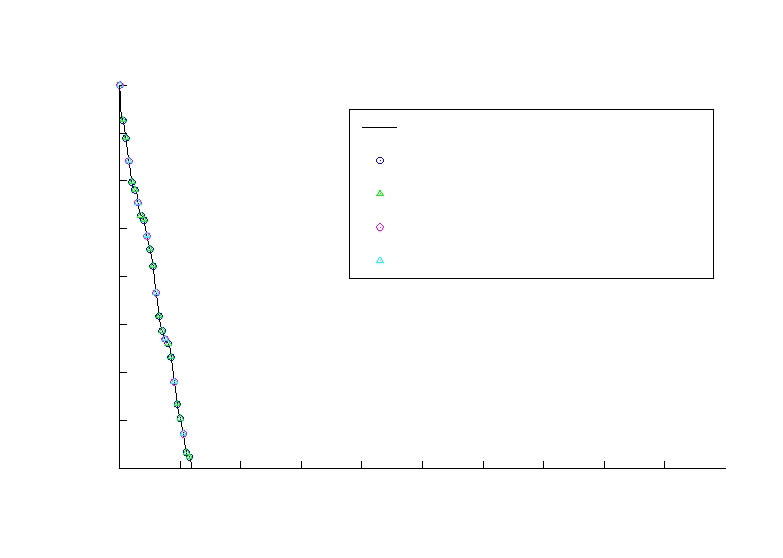
\includegraphics{watt1_ilu0}}%
    \gplfronttext
  \end{picture}%
\endgroup
}
	\caption{without basis vector scaling}
	\label{fig:watt1_ilu0}
\end{figure}
\begin{figure}
	\centering
	\resizebox{.9\textwidth}{!}{% GNUPLOT: LaTeX picture with Postscript
\begingroup
  \fontfamily{phv}%
  \selectfont
  \makeatletter
  \providecommand\color[2][]{%
    \GenericError{(gnuplot) \space\space\space\@spaces}{%
      Package color not loaded in conjunction with
      terminal option `colourtext'%
    }{See the gnuplot documentation for explanation.%
    }{Either use 'blacktext' in gnuplot or load the package
      color.sty in LaTeX.}%
    \renewcommand\color[2][]{}%
  }%
  \providecommand\includegraphics[2][]{%
    \GenericError{(gnuplot) \space\space\space\@spaces}{%
      Package graphicx or graphics not loaded%
    }{See the gnuplot documentation for explanation.%
    }{The gnuplot epslatex terminal needs graphicx.sty or graphics.sty.}%
    \renewcommand\includegraphics[2][]{}%
  }%
  \providecommand\rotatebox[2]{#2}%
  \@ifundefined{ifGPcolor}{%
    \newif\ifGPcolor
    \GPcolorfalse
  }{}%
  \@ifundefined{ifGPblacktext}{%
    \newif\ifGPblacktext
    \GPblacktexttrue
  }{}%
  % define a \g@addto@macro without @ in the name:
  \let\gplgaddtomacro\g@addto@macro
  % define empty templates for all commands taking text:
  \gdef\gplbacktext{}%
  \gdef\gplfronttext{}%
  \makeatother
  \ifGPblacktext
    % no textcolor at all
    \def\colorrgb#1{}%
    \def\colorgray#1{}%
  \else
    % gray or color?
    \ifGPcolor
      \def\colorrgb#1{\color[rgb]{#1}}%
      \def\colorgray#1{\color[gray]{#1}}%
      \expandafter\def\csname LTw\endcsname{\color{white}}%
      \expandafter\def\csname LTb\endcsname{\color{black}}%
      \expandafter\def\csname LTa\endcsname{\color{black}}%
      \expandafter\def\csname LT0\endcsname{\color[rgb]{1,0,0}}%
      \expandafter\def\csname LT1\endcsname{\color[rgb]{0,1,0}}%
      \expandafter\def\csname LT2\endcsname{\color[rgb]{0,0,1}}%
      \expandafter\def\csname LT3\endcsname{\color[rgb]{1,0,1}}%
      \expandafter\def\csname LT4\endcsname{\color[rgb]{0,1,1}}%
      \expandafter\def\csname LT5\endcsname{\color[rgb]{1,1,0}}%
      \expandafter\def\csname LT6\endcsname{\color[rgb]{0,0,0}}%
      \expandafter\def\csname LT7\endcsname{\color[rgb]{1,0.3,0}}%
      \expandafter\def\csname LT8\endcsname{\color[rgb]{0.5,0.5,0.5}}%
    \else
      % gray
      \def\colorrgb#1{\color{black}}%
      \def\colorgray#1{\color[gray]{#1}}%
      \expandafter\def\csname LTw\endcsname{\color{white}}%
      \expandafter\def\csname LTb\endcsname{\color{black}}%
      \expandafter\def\csname LTa\endcsname{\color{black}}%
      \expandafter\def\csname LT0\endcsname{\color{black}}%
      \expandafter\def\csname LT1\endcsname{\color{black}}%
      \expandafter\def\csname LT2\endcsname{\color{black}}%
      \expandafter\def\csname LT3\endcsname{\color{black}}%
      \expandafter\def\csname LT4\endcsname{\color{black}}%
      \expandafter\def\csname LT5\endcsname{\color{black}}%
      \expandafter\def\csname LT6\endcsname{\color{black}}%
      \expandafter\def\csname LT7\endcsname{\color{black}}%
      \expandafter\def\csname LT8\endcsname{\color{black}}%
    \fi
  \fi
    \setlength{\unitlength}{0.0500bp}%
    \ifx\gptboxheight\undefined%
      \newlength{\gptboxheight}%
      \newlength{\gptboxwidth}%
      \newsavebox{\gptboxtext}%
    \fi%
    \setlength{\fboxrule}{0.5pt}%
    \setlength{\fboxsep}{1pt}%
\begin{picture}(7200.00,5040.00)%
    \gplgaddtomacro\gplbacktext{%
      \csname LTb\endcsname%
      \put(726,704){\makebox(0,0)[r]{\strut{}\footnotesize -4}}%
      \put(726,1623){\makebox(0,0)[r]{\strut{}\footnotesize -3}}%
      \put(726,2542){\makebox(0,0)[r]{\strut{}\footnotesize -2}}%
      \put(726,3460){\makebox(0,0)[r]{\strut{}\footnotesize -1}}%
      \put(726,4379){\makebox(0,0)[r]{\strut{}\footnotesize 0}}%
      \put(1453,484){\makebox(0,0){\strut{}\footnotesize 100}}%
      \put(2047,484){\makebox(0,0){\strut{}\footnotesize 200}}%
      \put(2642,484){\makebox(0,0){\strut{}\footnotesize 300}}%
      \put(3236,484){\makebox(0,0){\strut{}\footnotesize 400}}%
      \put(3831,484){\makebox(0,0){\strut{}\footnotesize 500}}%
      \put(4425,484){\makebox(0,0){\strut{}\footnotesize 600}}%
      \put(5020,484){\makebox(0,0){\strut{}\footnotesize 700}}%
      \put(5614,484){\makebox(0,0){\strut{}\footnotesize 800}}%
      \put(6209,484){\makebox(0,0){\strut{}\footnotesize 900}}%
			\put(6803,484){\makebox(0,0){\strut{}\footnotesize 1000}}%
    }%
    \gplgaddtomacro\gplfronttext{%
      \csname LTb\endcsname%
      \put(352,2541){\rotatebox{-270}{\makebox(0,0){\strut{}\footnotesize Residual 2-norm, log scale}}}%
      \put(3830,154){\makebox(0,0){\strut{}\footnotesize Iteration count}}%
      \put(3830,4709){\makebox(0,0){\strut{}\shortstack{pwtk}}}%
      \csname LTb\endcsname%
      \put(2591,4161){\makebox(0,0)[l]{\strut{}\scriptsize GMRES(20)}}%
      \csname LTb\endcsname%
      \put(2591,3842){\makebox(0,0)[l]{\strut{}\begin{minipage}[l]{.95\textwidth} \scriptsize Monomial-GMRES(5,4) \newline \tiny min, max basis rcond \#: 3.47e-33, 2.51e-32\end{minipage}}}%
      \csname LTb\endcsname%
      \put(2591,3523){\makebox(0,0)[l]{\strut{}\begin{minipage}[l]{.95\textwidth} \scriptsize Newton-GMRES(5,4) \newline \tiny min, max basis rcond \#: 9.33e-32, 8.36e-30\end{minipage}}}%
      \csname LTb\endcsname%
      \put(2591,3204){\makebox(0,0)[l]{\strut{}\begin{minipage}[l]{.95\textwidth} \scriptsize Monomial-GMRES(10,2) \newline \tiny min, max basis rcond \#: 3.61e-72, 2.91e-71\end{minipage}}}%
      \csname LTb\endcsname%
      \put(2591,2885){\makebox(0,0)[l]{\strut{}\begin{minipage}[l]{.95\textwidth} \scriptsize Newton-GMRES(10,2) \newline \tiny min, max basis rcond \#: 5.92e-68, 5.99e-66\end{minipage}}}%
    }%
    \gplbacktext
    \put(0,0){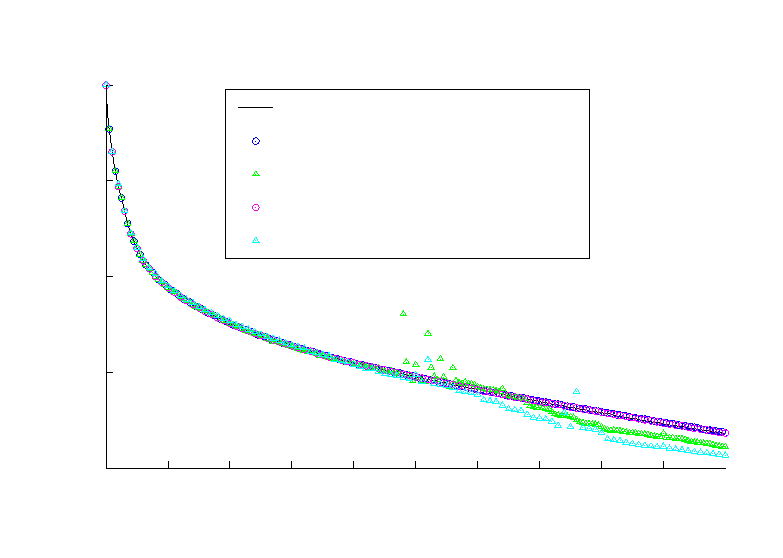
\includegraphics{pwtk_noscale}}%
    \gplfronttext
  \end{picture}%
\endgroup
}
	\caption{•••}
	\label{fig:pwtk_noscale}
\end{figure}
\begin{figure}
	\centering
	\resizebox{.9\textwidth}{!}{% GNUPLOT: LaTeX picture with Postscript
\begingroup
  \fontfamily{phv}%
  \selectfont
  \makeatletter
  \providecommand\color[2][]{%
    \GenericError{(gnuplot) \space\space\space\@spaces}{%
      Package color not loaded in conjunction with
      terminal option `colourtext'%
    }{See the gnuplot documentation for explanation.%
    }{Either use 'blacktext' in gnuplot or load the package
      color.sty in LaTeX.}%
    \renewcommand\color[2][]{}%
  }%
  \providecommand\includegraphics[2][]{%
    \GenericError{(gnuplot) \space\space\space\@spaces}{%
      Package graphicx or graphics not loaded%
    }{See the gnuplot documentation for explanation.%
    }{The gnuplot epslatex terminal needs graphicx.sty or graphics.sty.}%
    \renewcommand\includegraphics[2][]{}%
  }%
  \providecommand\rotatebox[2]{#2}%
  \@ifundefined{ifGPcolor}{%
    \newif\ifGPcolor
    \GPcolorfalse
  }{}%
  \@ifundefined{ifGPblacktext}{%
    \newif\ifGPblacktext
    \GPblacktexttrue
  }{}%
  % define a \g@addto@macro without @ in the name:
  \let\gplgaddtomacro\g@addto@macro
  % define empty templates for all commands taking text:
  \gdef\gplbacktext{}%
  \gdef\gplfronttext{}%
  \makeatother
  \ifGPblacktext
    % no textcolor at all
    \def\colorrgb#1{}%
    \def\colorgray#1{}%
  \else
    % gray or color?
    \ifGPcolor
      \def\colorrgb#1{\color[rgb]{#1}}%
      \def\colorgray#1{\color[gray]{#1}}%
      \expandafter\def\csname LTw\endcsname{\color{white}}%
      \expandafter\def\csname LTb\endcsname{\color{black}}%
      \expandafter\def\csname LTa\endcsname{\color{black}}%
      \expandafter\def\csname LT0\endcsname{\color[rgb]{1,0,0}}%
      \expandafter\def\csname LT1\endcsname{\color[rgb]{0,1,0}}%
      \expandafter\def\csname LT2\endcsname{\color[rgb]{0,0,1}}%
      \expandafter\def\csname LT3\endcsname{\color[rgb]{1,0,1}}%
      \expandafter\def\csname LT4\endcsname{\color[rgb]{0,1,1}}%
      \expandafter\def\csname LT5\endcsname{\color[rgb]{1,1,0}}%
      \expandafter\def\csname LT6\endcsname{\color[rgb]{0,0,0}}%
      \expandafter\def\csname LT7\endcsname{\color[rgb]{1,0.3,0}}%
      \expandafter\def\csname LT8\endcsname{\color[rgb]{0.5,0.5,0.5}}%
    \else
      % gray
      \def\colorrgb#1{\color{black}}%
      \def\colorgray#1{\color[gray]{#1}}%
      \expandafter\def\csname LTw\endcsname{\color{white}}%
      \expandafter\def\csname LTb\endcsname{\color{black}}%
      \expandafter\def\csname LTa\endcsname{\color{black}}%
      \expandafter\def\csname LT0\endcsname{\color{black}}%
      \expandafter\def\csname LT1\endcsname{\color{black}}%
      \expandafter\def\csname LT2\endcsname{\color{black}}%
      \expandafter\def\csname LT3\endcsname{\color{black}}%
      \expandafter\def\csname LT4\endcsname{\color{black}}%
      \expandafter\def\csname LT5\endcsname{\color{black}}%
      \expandafter\def\csname LT6\endcsname{\color{black}}%
      \expandafter\def\csname LT7\endcsname{\color{black}}%
      \expandafter\def\csname LT8\endcsname{\color{black}}%
    \fi
  \fi
    \setlength{\unitlength}{0.0500bp}%
    \ifx\gptboxheight\undefined%
      \newlength{\gptboxheight}%
      \newlength{\gptboxwidth}%
      \newsavebox{\gptboxtext}%
    \fi%
    \setlength{\fboxrule}{0.5pt}%
    \setlength{\fboxsep}{1pt}%
\begin{picture}(7200.00,5040.00)%
    \gplgaddtomacro\gplbacktext{%
      \csname LTb\endcsname%
      \put(726,704){\makebox(0,0)[r]{\strut{}\footnotesize -4}}%
      \put(726,1623){\makebox(0,0)[r]{\strut{}\footnotesize -3}}%
      \put(726,2542){\makebox(0,0)[r]{\strut{}\footnotesize -2}}%
      \put(726,3460){\makebox(0,0)[r]{\strut{}\footnotesize -1}}%
      \put(726,4379){\makebox(0,0)[r]{\strut{}\footnotesize 0}}%
      \put(1453,484){\makebox(0,0){\strut{}\footnotesize 100}}%
      \put(2047,484){\makebox(0,0){\strut{}\footnotesize 200}}%
      \put(2642,484){\makebox(0,0){\strut{}\footnotesize 300}}%
      \put(3236,484){\makebox(0,0){\strut{}\footnotesize 400}}%
      \put(3831,484){\makebox(0,0){\strut{}\footnotesize 500}}%
      \put(4425,484){\makebox(0,0){\strut{}\footnotesize 600}}%
      \put(5020,484){\makebox(0,0){\strut{}\footnotesize 700}}%
      \put(5614,484){\makebox(0,0){\strut{}\footnotesize 800}}%
      \put(6209,484){\makebox(0,0){\strut{}\footnotesize 900}}%
			\put(6803,484){\makebox(0,0){\strut{}\footnotesize 1000}}%
    }%
    \gplgaddtomacro\gplfronttext{%
      \csname LTb\endcsname%
      \put(352,2541){\rotatebox{-270}{\makebox(0,0){\strut{}\footnotesize Residual 2-norm, log scale}}}%
      \put(3830,154){\makebox(0,0){\strut{}\footnotesize Iteration count}}%
      \put(3830,4709){\makebox(0,0){\strut{}\shortstack{pwtk}}}%
      \csname LTb\endcsname%
      \put(2591,4161){\makebox(0,0)[l]{\strut{}\scriptsize GMRES(20)}}%
      \csname LTb\endcsname%
      \put(2591,3842){\makebox(0,0)[l]{\strut{}\begin{minipage}[l]{.95\textwidth} \scriptsize Monomial-GMRES(5,4) \newline \tiny min, max basis rcond \#: 3.08e-11, 3.13e-10\end{minipage}}}%
      \csname LTb\endcsname%
      \put(2591,3523){\makebox(0,0)[l]{\strut{}\begin{minipage}[l]{.95\textwidth} \scriptsize Newton-GMRES(5,4) \newline \tiny min, max basis rcond \#: 7.48e-16, 2.46e-08\end{minipage}}}%
      \csname LTb\endcsname%
      \put(2591,3204){\makebox(0,0)[l]{\strut{}\begin{minipage}[l]{.95\textwidth} \scriptsize Monomial-GMRES(10,2) \newline \tiny min, max basis rcond \#: 3.27e-14, 3.84e-13\end{minipage}}}%
      \csname LTb\endcsname%
      \put(2591,2885){\makebox(0,0)[l]{\strut{}\begin{minipage}[l]{.95\textwidth} \scriptsize Newton-GMRES(10,2) \newline \tiny min, max basis rcond \#: 1.38e-23, 6.42e-23\end{minipage}}}%
    }%
    \gplbacktext
    \put(0,0){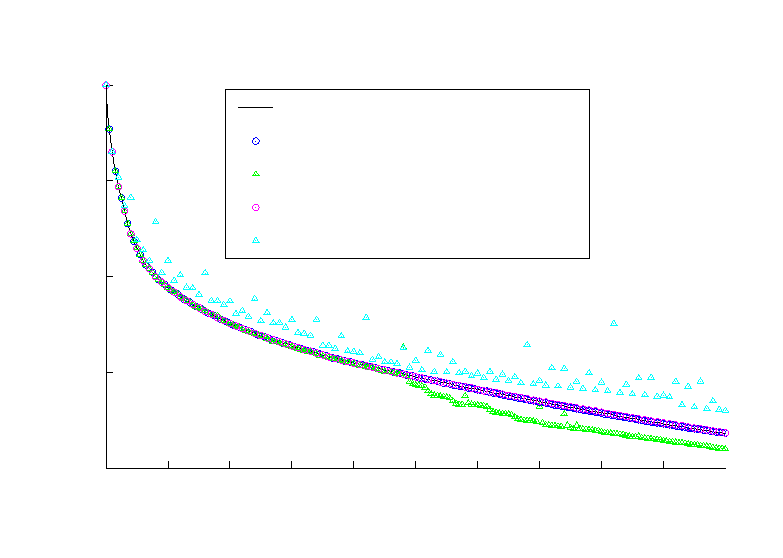
\includegraphics{pwtk_scale}}%
    \gplfronttext
  \end{picture}%
\endgroup
}
	\caption{•••}
	\label{fig:pwtk_scale}
\end{figure}
\begin{figure}
	\centering
	\resizebox{.9\textwidth}{!}{% GNUPLOT: LaTeX picture with Postscript
\begingroup
  \fontfamily{phv}%
  \selectfont
  \makeatletter
  \providecommand\color[2][]{%
    \GenericError{(gnuplot) \space\space\space\@spaces}{%
      Package color not loaded in conjunction with
      terminal option `colourtext'%
    }{See the gnuplot documentation for explanation.%
    }{Either use 'blacktext' in gnuplot or load the package
      color.sty in LaTeX.}%
    \renewcommand\color[2][]{}%
  }%
  \providecommand\includegraphics[2][]{%
    \GenericError{(gnuplot) \space\space\space\@spaces}{%
      Package graphicx or graphics not loaded%
    }{See the gnuplot documentation for explanation.%
    }{The gnuplot epslatex terminal needs graphicx.sty or graphics.sty.}%
    \renewcommand\includegraphics[2][]{}%
  }%
  \providecommand\rotatebox[2]{#2}%
  \@ifundefined{ifGPcolor}{%
    \newif\ifGPcolor
    \GPcolorfalse
  }{}%
  \@ifundefined{ifGPblacktext}{%
    \newif\ifGPblacktext
    \GPblacktexttrue
  }{}%
  % define a \g@addto@macro without @ in the name:
  \let\gplgaddtomacro\g@addto@macro
  % define empty templates for all commands taking text:
  \gdef\gplbacktext{}%
  \gdef\gplfronttext{}%
  \makeatother
  \ifGPblacktext
    % no textcolor at all
    \def\colorrgb#1{}%
    \def\colorgray#1{}%
  \else
    % gray or color?
    \ifGPcolor
      \def\colorrgb#1{\color[rgb]{#1}}%
      \def\colorgray#1{\color[gray]{#1}}%
      \expandafter\def\csname LTw\endcsname{\color{white}}%
      \expandafter\def\csname LTb\endcsname{\color{black}}%
      \expandafter\def\csname LTa\endcsname{\color{black}}%
      \expandafter\def\csname LT0\endcsname{\color[rgb]{1,0,0}}%
      \expandafter\def\csname LT1\endcsname{\color[rgb]{0,1,0}}%
      \expandafter\def\csname LT2\endcsname{\color[rgb]{0,0,1}}%
      \expandafter\def\csname LT3\endcsname{\color[rgb]{1,0,1}}%
      \expandafter\def\csname LT4\endcsname{\color[rgb]{0,1,1}}%
      \expandafter\def\csname LT5\endcsname{\color[rgb]{1,1,0}}%
      \expandafter\def\csname LT6\endcsname{\color[rgb]{0,0,0}}%
      \expandafter\def\csname LT7\endcsname{\color[rgb]{1,0.3,0}}%
      \expandafter\def\csname LT8\endcsname{\color[rgb]{0.5,0.5,0.5}}%
    \else
      % gray
      \def\colorrgb#1{\color{black}}%
      \def\colorgray#1{\color[gray]{#1}}%
      \expandafter\def\csname LTw\endcsname{\color{white}}%
      \expandafter\def\csname LTb\endcsname{\color{black}}%
      \expandafter\def\csname LTa\endcsname{\color{black}}%
      \expandafter\def\csname LT0\endcsname{\color{black}}%
      \expandafter\def\csname LT1\endcsname{\color{black}}%
      \expandafter\def\csname LT2\endcsname{\color{black}}%
      \expandafter\def\csname LT3\endcsname{\color{black}}%
      \expandafter\def\csname LT4\endcsname{\color{black}}%
      \expandafter\def\csname LT5\endcsname{\color{black}}%
      \expandafter\def\csname LT6\endcsname{\color{black}}%
      \expandafter\def\csname LT7\endcsname{\color{black}}%
      \expandafter\def\csname LT8\endcsname{\color{black}}%
    \fi
  \fi
    \setlength{\unitlength}{0.0500bp}%
    \ifx\gptboxheight\undefined%
      \newlength{\gptboxheight}%
      \newlength{\gptboxwidth}%
      \newsavebox{\gptboxtext}%
    \fi%
    \setlength{\fboxrule}{0.5pt}%
    \setlength{\fboxsep}{1pt}%
\begin{picture}(7200.00,5040.00)%
    \gplgaddtomacro\gplbacktext{%
      \csname LTb\endcsname%
      \put(858,4195){\makebox(0,0)[r]{\strut{}\footnotesize -16}}%
      \put(858,4207){\makebox(0,0)[r]{\strut{}\footnotesize -15}}%
      \put(858,4218){\makebox(0,0)[r]{\strut{}\footnotesize -14}}%
      \put(858,4230){\makebox(0,0)[r]{\strut{}\footnotesize -13}}%
      \put(858,4241){\makebox(0,0)[r]{\strut{}\footnotesize -12}}%
      \put(858,4253){\makebox(0,0)[r]{\strut{}\footnotesize -11}}%
      \put(858,4264){\makebox(0,0)[r]{\strut{}\footnotesize -10}}%
      \put(858,4276){\makebox(0,0)[r]{\strut{}\footnotesize -9}}%
      \put(858,4287){\makebox(0,0)[r]{\strut{}\footnotesize -8}}%
      \put(858,4299){\makebox(0,0)[r]{\strut{}\footnotesize -7}}%
      \put(858,4310){\makebox(0,0)[r]{\strut{}\footnotesize -6}}%
      \put(858,4322){\makebox(0,0)[r]{\strut{}\footnotesize -5}}%
      \put(858,4333){\makebox(0,0)[r]{\strut{}\footnotesize -4}}%
      \put(858,4345){\makebox(0,0)[r]{\strut{}\footnotesize -3}}%
      \put(858,4356){\makebox(0,0)[r]{\strut{}\footnotesize -2}}%
      \put(858,4368){\makebox(0,0)[r]{\strut{}\footnotesize -1}}%
      \put(858,4379){\makebox(0,0)[r]{\strut{}\footnotesize 0}}%
      \put(1898,484){\makebox(0,0){\strut{}\footnotesize 5}}%
      \put(2807,484){\makebox(0,0){\strut{}\footnotesize 10}}%
      \put(3715,484){\makebox(0,0){\strut{}\footnotesize 15}}%
      \put(4623,484){\makebox(0,0){\strut{}\footnotesize 20}}%
      \put(5531,484){\makebox(0,0){\strut{}\footnotesize 25}}%
      \put(6440,484){\makebox(0,0){\strut{}\footnotesize 30}}%
    }%
    \gplgaddtomacro\gplfronttext{%
      \csname LTb\endcsname%
      \put(352,2541){\rotatebox{-270}{\makebox(0,0){\strut{}\footnotesize Residual 2-norm, log scale}}}%
      \put(3896,154){\makebox(0,0){\strut{}\footnotesize Iteration count}}%
      \put(3896,4709){\makebox(0,0){\strut{}\shortstack{bmw}}}%
      \csname LTb\endcsname%
      \put(4295,2217){\makebox(0,0)[l]{\strut{}\scriptsize GMRES(20)}}%
      \csname LTb\endcsname%
      \put(4295,1898){\makebox(0,0)[l]{\strut{}\begin{minipage}[l]{.95\textwidth} \scriptsize Monomial-GMRES(5,4) \newline \tiny min, max basis rcond \#: 1.87e-01, 1.87e-01\end{minipage}}}%
      \csname LTb\endcsname%
      \put(4295,1579){\makebox(0,0)[l]{\strut{}\begin{minipage}[l]{.95\textwidth} \scriptsize Newton-GMRES(5,4) \newline \tiny min, max basis rcond \#: 1.25e-16, 1.25e-16\end{minipage}}}%
      \csname LTb\endcsname%
      \put(4295,1260){\makebox(0,0)[l]{\strut{}\begin{minipage}[l]{.95\textwidth} \scriptsize Monomial-GMRES(10,2) \newline \tiny min, max basis rcond \#: 1.40e-01, 1.40e-01\end{minipage}}}%
      \csname LTb\endcsname%
      \put(4295,941){\makebox(0,0)[l]{\strut{}\begin{minipage}[l]{.95\textwidth} \scriptsize Newton-GMRES(10,2) \newline \tiny min, max basis rcond \#: 1.69e-17, 1.69e-17\end{minipage}}}%
    }%
    \gplbacktext
    \put(0,0){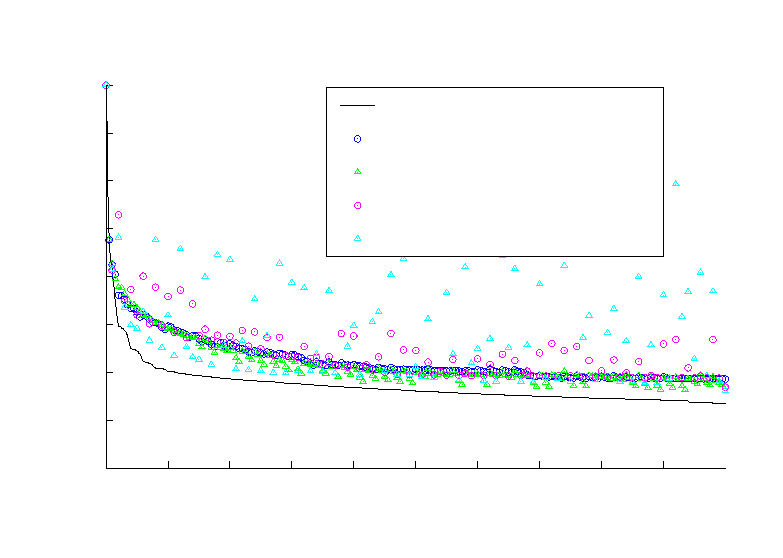
\includegraphics{bmw7st1}}%
    \gplfronttext
  \end{picture}%
\endgroup
}
	\caption{•••}
	\label{fig:bmw7st1}
\end{figure}
\begin{figure}
	\centering
	\resizebox{.9\textwidth}{!}{% GNUPLOT: LaTeX picture with Postscript
\begingroup
  \fontfamily{phv}%
  \selectfont
  \makeatletter
  \providecommand\color[2][]{%
    \GenericError{(gnuplot) \space\space\space\@spaces}{%
      Package color not loaded in conjunction with
      terminal option `colourtext'%
    }{See the gnuplot documentation for explanation.%
    }{Either use 'blacktext' in gnuplot or load the package
      color.sty in LaTeX.}%
    \renewcommand\color[2][]{}%
  }%
  \providecommand\includegraphics[2][]{%
    \GenericError{(gnuplot) \space\space\space\@spaces}{%
      Package graphicx or graphics not loaded%
    }{See the gnuplot documentation for explanation.%
    }{The gnuplot epslatex terminal needs graphicx.sty or graphics.sty.}%
    \renewcommand\includegraphics[2][]{}%
  }%
  \providecommand\rotatebox[2]{#2}%
  \@ifundefined{ifGPcolor}{%
    \newif\ifGPcolor
    \GPcolorfalse
  }{}%
  \@ifundefined{ifGPblacktext}{%
    \newif\ifGPblacktext
    \GPblacktexttrue
  }{}%
  % define a \g@addto@macro without @ in the name:
  \let\gplgaddtomacro\g@addto@macro
  % define empty templates for all commands taking text:
  \gdef\gplbacktext{}%
  \gdef\gplfronttext{}%
  \makeatother
  \ifGPblacktext
    % no textcolor at all
    \def\colorrgb#1{}%
    \def\colorgray#1{}%
  \else
    % gray or color?
    \ifGPcolor
      \def\colorrgb#1{\color[rgb]{#1}}%
      \def\colorgray#1{\color[gray]{#1}}%
      \expandafter\def\csname LTw\endcsname{\color{white}}%
      \expandafter\def\csname LTb\endcsname{\color{black}}%
      \expandafter\def\csname LTa\endcsname{\color{black}}%
      \expandafter\def\csname LT0\endcsname{\color[rgb]{1,0,0}}%
      \expandafter\def\csname LT1\endcsname{\color[rgb]{0,1,0}}%
      \expandafter\def\csname LT2\endcsname{\color[rgb]{0,0,1}}%
      \expandafter\def\csname LT3\endcsname{\color[rgb]{1,0,1}}%
      \expandafter\def\csname LT4\endcsname{\color[rgb]{0,1,1}}%
      \expandafter\def\csname LT5\endcsname{\color[rgb]{1,1,0}}%
      \expandafter\def\csname LT6\endcsname{\color[rgb]{0,0,0}}%
      \expandafter\def\csname LT7\endcsname{\color[rgb]{1,0.3,0}}%
      \expandafter\def\csname LT8\endcsname{\color[rgb]{0.5,0.5,0.5}}%
    \else
      % gray
      \def\colorrgb#1{\color{black}}%
      \def\colorgray#1{\color[gray]{#1}}%
      \expandafter\def\csname LTw\endcsname{\color{white}}%
      \expandafter\def\csname LTb\endcsname{\color{black}}%
      \expandafter\def\csname LTa\endcsname{\color{black}}%
      \expandafter\def\csname LT0\endcsname{\color{black}}%
      \expandafter\def\csname LT1\endcsname{\color{black}}%
      \expandafter\def\csname LT2\endcsname{\color{black}}%
      \expandafter\def\csname LT3\endcsname{\color{black}}%
      \expandafter\def\csname LT4\endcsname{\color{black}}%
      \expandafter\def\csname LT5\endcsname{\color{black}}%
      \expandafter\def\csname LT6\endcsname{\color{black}}%
      \expandafter\def\csname LT7\endcsname{\color{black}}%
      \expandafter\def\csname LT8\endcsname{\color{black}}%
    \fi
  \fi
    \setlength{\unitlength}{0.0500bp}%
    \ifx\gptboxheight\undefined%
      \newlength{\gptboxheight}%
      \newlength{\gptboxwidth}%
      \newsavebox{\gptboxtext}%
    \fi%
    \setlength{\fboxrule}{0.5pt}%
    \setlength{\fboxsep}{1pt}%
\begin{picture}(7200.00,5040.00)%
    \gplgaddtomacro\gplbacktext{%
      \csname LTb\endcsname%
      \put(726,704){\makebox(0,0)[r]{\strut{}\footnotesize -8}}%
      \put(726,1163){\makebox(0,0)[r]{\strut{}\footnotesize -7}}%
      \put(726,1623){\makebox(0,0)[r]{\strut{}\footnotesize -6}}%
      \put(726,2082){\makebox(0,0)[r]{\strut{}\footnotesize -5}}%
      \put(726,2542){\makebox(0,0)[r]{\strut{}\footnotesize -4}}%
      \put(726,3001){\makebox(0,0)[r]{\strut{}\footnotesize -3}}%
      \put(726,3460){\makebox(0,0)[r]{\strut{}\footnotesize -2}}%
      \put(726,3920){\makebox(0,0)[r]{\strut{}\footnotesize -1}}%
      \put(726,4379){\makebox(0,0)[r]{\strut{}\footnotesize 0}}%
      \put(1453,484){\makebox(0,0){\strut{}\footnotesize 100}}%
      \put(2047,484){\makebox(0,0){\strut{}\footnotesize 200}}%
      \put(2642,484){\makebox(0,0){\strut{}\footnotesize 300}}%
      \put(3236,484){\makebox(0,0){\strut{}\footnotesize 400}}%
      \put(3831,484){\makebox(0,0){\strut{}\footnotesize 500}}%
      \put(4425,484){\makebox(0,0){\strut{}\footnotesize 600}}%
      \put(5020,484){\makebox(0,0){\strut{}\footnotesize 700}}%
      \put(5614,484){\makebox(0,0){\strut{}\footnotesize 800}}%
      \put(6209,484){\makebox(0,0){\strut{}\footnotesize 900}}%
    }%
    \gplgaddtomacro\gplfronttext{%
      \csname LTb\endcsname%
      \put(352,2541){\rotatebox{-270}{\makebox(0,0){\strut{}\footnotesize Residual 2-norm, log scale}}}%
      \put(3830,154){\makebox(0,0){\strut{}\footnotesize Iteration count}}%
      \put(3830,4709){\makebox(0,0){\strut{}\shortstack{bmw}}}%
      \csname LTb\endcsname%
      \put(3833,4182){\makebox(0,0)[l]{\strut{}\scriptsize GMRES(20)}}%
      \csname LTb\endcsname%
      \put(3833,3863){\makebox(0,0)[l]{\strut{}\begin{minipage}[l]{.95\textwidth} \scriptsize Monomial-GMRES(5,4) \newline \tiny min, max basis rcond \#: 1.51e-12, 8.52e-06\end{minipage}}}%
      \csname LTb\endcsname%
      \put(3833,3544){\makebox(0,0)[l]{\strut{}\begin{minipage}[l]{.95\textwidth} \scriptsize Newton-GMRES(5,4) \newline \tiny min, max basis rcond \#: 1.11e-12, 8.18e-04\end{minipage}}}%
      \csname LTb\endcsname%
      \put(3833,3225){\makebox(0,0)[l]{\strut{}\begin{minipage}[l]{.95\textwidth} \scriptsize Monomial-GMRES(10,2) \newline \tiny min, max basis rcond \#: 2.02e-18, 4.03e-15\end{minipage}}}%
      \csname LTb\endcsname%
      \put(3833,2906){\makebox(0,0)[l]{\strut{}\begin{minipage}[l]{.95\textwidth} \scriptsize Newton-GMRES(10,2) \newline \tiny min, max basis rcond \#: 3.54e-17, 4.84e-15\end{minipage}}}%
    }%
    \gplbacktext
    \put(0,0){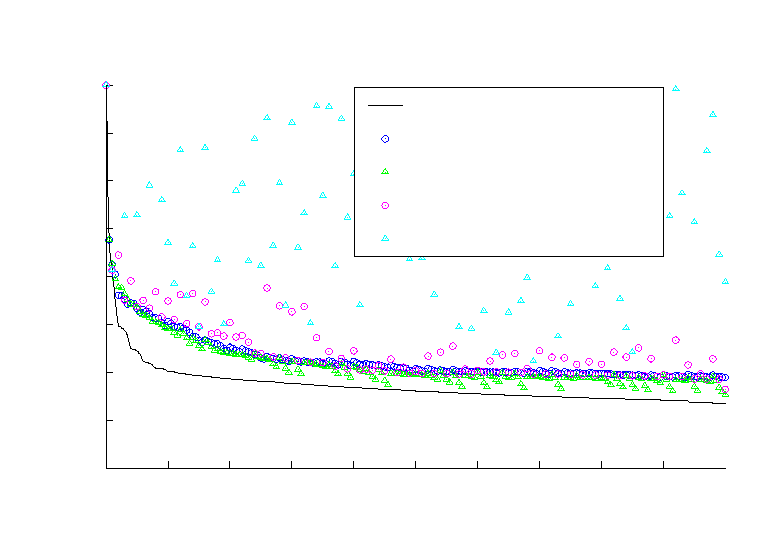
\includegraphics{bmw7st1_scale}}%
    \gplfronttext
  \end{picture}%
\endgroup
}
	\caption{•••}
	\label{fig:bmw7st1_scale}
\end{figure}
\begin{figure}
	\centering
	\resizebox{.9\textwidth}{!}{% GNUPLOT: LaTeX picture with Postscript
\begingroup
  \fontfamily{phv}%
  \selectfont
  \makeatletter
  \providecommand\color[2][]{%
    \GenericError{(gnuplot) \space\space\space\@spaces}{%
      Package color not loaded in conjunction with
      terminal option `colourtext'%
    }{See the gnuplot documentation for explanation.%
    }{Either use 'blacktext' in gnuplot or load the package
      color.sty in LaTeX.}%
    \renewcommand\color[2][]{}%
  }%
  \providecommand\includegraphics[2][]{%
    \GenericError{(gnuplot) \space\space\space\@spaces}{%
      Package graphicx or graphics not loaded%
    }{See the gnuplot documentation for explanation.%
    }{The gnuplot epslatex terminal needs graphicx.sty or graphics.sty.}%
    \renewcommand\includegraphics[2][]{}%
  }%
  \providecommand\rotatebox[2]{#2}%
  \@ifundefined{ifGPcolor}{%
    \newif\ifGPcolor
    \GPcolorfalse
  }{}%
  \@ifundefined{ifGPblacktext}{%
    \newif\ifGPblacktext
    \GPblacktexttrue
  }{}%
  % define a \g@addto@macro without @ in the name:
  \let\gplgaddtomacro\g@addto@macro
  % define empty templates for all commands taking text:
  \gdef\gplbacktext{}%
  \gdef\gplfronttext{}%
  \makeatother
  \ifGPblacktext
    % no textcolor at all
    \def\colorrgb#1{}%
    \def\colorgray#1{}%
  \else
    % gray or color?
    \ifGPcolor
      \def\colorrgb#1{\color[rgb]{#1}}%
      \def\colorgray#1{\color[gray]{#1}}%
      \expandafter\def\csname LTw\endcsname{\color{white}}%
      \expandafter\def\csname LTb\endcsname{\color{black}}%
      \expandafter\def\csname LTa\endcsname{\color{black}}%
      \expandafter\def\csname LT0\endcsname{\color[rgb]{1,0,0}}%
      \expandafter\def\csname LT1\endcsname{\color[rgb]{0,1,0}}%
      \expandafter\def\csname LT2\endcsname{\color[rgb]{0,0,1}}%
      \expandafter\def\csname LT3\endcsname{\color[rgb]{1,0,1}}%
      \expandafter\def\csname LT4\endcsname{\color[rgb]{0,1,1}}%
      \expandafter\def\csname LT5\endcsname{\color[rgb]{1,1,0}}%
      \expandafter\def\csname LT6\endcsname{\color[rgb]{0,0,0}}%
      \expandafter\def\csname LT7\endcsname{\color[rgb]{1,0.3,0}}%
      \expandafter\def\csname LT8\endcsname{\color[rgb]{0.5,0.5,0.5}}%
    \else
      % gray
      \def\colorrgb#1{\color{black}}%
      \def\colorgray#1{\color[gray]{#1}}%
      \expandafter\def\csname LTw\endcsname{\color{white}}%
      \expandafter\def\csname LTb\endcsname{\color{black}}%
      \expandafter\def\csname LTa\endcsname{\color{black}}%
      \expandafter\def\csname LT0\endcsname{\color{black}}%
      \expandafter\def\csname LT1\endcsname{\color{black}}%
      \expandafter\def\csname LT2\endcsname{\color{black}}%
      \expandafter\def\csname LT3\endcsname{\color{black}}%
      \expandafter\def\csname LT4\endcsname{\color{black}}%
      \expandafter\def\csname LT5\endcsname{\color{black}}%
      \expandafter\def\csname LT6\endcsname{\color{black}}%
      \expandafter\def\csname LT7\endcsname{\color{black}}%
      \expandafter\def\csname LT8\endcsname{\color{black}}%
    \fi
  \fi
    \setlength{\unitlength}{0.0500bp}%
    \ifx\gptboxheight\undefined%
      \newlength{\gptboxheight}%
      \newlength{\gptboxwidth}%
      \newsavebox{\gptboxtext}%
    \fi%
    \setlength{\fboxrule}{0.5pt}%
    \setlength{\fboxsep}{1pt}%
\begin{picture}(7200.00,5040.00)%
    \gplgaddtomacro\gplbacktext{%
      \csname LTb\endcsname%
      \put(726,704){\makebox(0,0)[r]{\strut{}\footnotesize -6}}%
      \put(726,1316){\makebox(0,0)[r]{\strut{}\footnotesize -5}}%
      \put(726,1929){\makebox(0,0)[r]{\strut{}\footnotesize -4}}%
      \put(726,2542){\makebox(0,0)[r]{\strut{}\footnotesize -3}}%
      \put(726,3154){\makebox(0,0)[r]{\strut{}\footnotesize -2}}%
      \put(726,3767){\makebox(0,0)[r]{\strut{}\footnotesize -1}}%
      \put(726,4379){\makebox(0,0)[r]{\strut{}\footnotesize 0}}%
      \put(1453,484){\makebox(0,0){\strut{}\footnotesize 100}}%
      \put(2047,484){\makebox(0,0){\strut{}\footnotesize 200}}%
      \put(2642,484){\makebox(0,0){\strut{}\footnotesize 300}}%
      \put(3236,484){\makebox(0,0){\strut{}\footnotesize 400}}%
      \put(3831,484){\makebox(0,0){\strut{}\footnotesize 500}}%
      \put(4425,484){\makebox(0,0){\strut{}\footnotesize 600}}%
      \put(5020,484){\makebox(0,0){\strut{}\footnotesize 700}}%
      \put(5614,484){\makebox(0,0){\strut{}\footnotesize 800}}%
      \put(6209,484){\makebox(0,0){\strut{}\footnotesize 900}}%
			\put(6803,484){\makebox(0,0){\strut{}\footnotesize 1000}}%
    }%
    \gplgaddtomacro\gplfronttext{%
      \csname LTb\endcsname%
      \put(352,2541){\rotatebox{-270}{\makebox(0,0){\strut{}\footnotesize Residual 2-norm, log scale}}}%
      \put(3830,154){\makebox(0,0){\strut{}\footnotesize Iteration count}}%
      \put(3830,4709){\makebox(0,0){\strut{}\shortstack{Xenon2}}}%
      \csname LTb\endcsname%
      \put(2380,3775){\makebox(0,0)[l]{\strut{}\scriptsize GMRES(20)}}%
      \csname LTb\endcsname%
      \put(2380,3456){\makebox(0,0)[l]{\strut{}\begin{minipage}[l]{.95\textwidth} \scriptsize Monomial-GMRES(5,4) \newline \tiny min, max basis rcond \#: 2.43e-117, 3.02e-117\end{minipage}}}%
      \csname LTb\endcsname%
      \put(2380,3137){\makebox(0,0)[l]{\strut{}\begin{minipage}[l]{.95\textwidth} \scriptsize Newton-GMRES(5,4) \newline \tiny min, max basis rcond \#: 5.37e-114, 1.59e-113\end{minipage}}}%
      \csname LTb\endcsname%
      \put(2380,2818){\makebox(0,0)[l]{\strut{}\begin{minipage}[l]{.95\textwidth} \scriptsize Monomial-GMRES(10,2) \newline \tiny min, max basis rcond \#: 1.17e-261, 1.40e-261\end{minipage}}}%
      \csname LTb\endcsname%
      \put(2380,2499){\makebox(0,0)[l]{\strut{}\begin{minipage}[l]{.95\textwidth} \scriptsize Newton-GMRES(10,2) \newline \tiny min, max basis rcond \#: 5.97e-255, 2.80e-254\end{minipage}}}%
    }%
    \gplbacktext
    \put(0,0){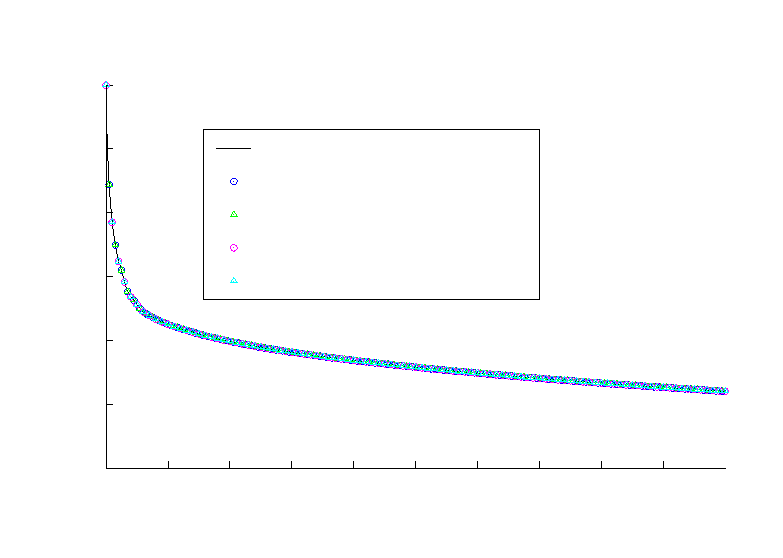
\includegraphics{xenon2}}%
    \gplfronttext
  \end{picture}%
\endgroup
}
	\caption{•••}
	\label{fig:xenon2}
\end{figure}
\begin{figure}
	\centering
	\resizebox{.9\textwidth}{!}{% GNUPLOT: LaTeX picture with Postscript
\begingroup
  \fontfamily{phv}%
  \selectfont
  \makeatletter
  \providecommand\color[2][]{%
    \GenericError{(gnuplot) \space\space\space\@spaces}{%
      Package color not loaded in conjunction with
      terminal option `colourtext'%
    }{See the gnuplot documentation for explanation.%
    }{Either use 'blacktext' in gnuplot or load the package
      color.sty in LaTeX.}%
    \renewcommand\color[2][]{}%
  }%
  \providecommand\includegraphics[2][]{%
    \GenericError{(gnuplot) \space\space\space\@spaces}{%
      Package graphicx or graphics not loaded%
    }{See the gnuplot documentation for explanation.%
    }{The gnuplot epslatex terminal needs graphicx.sty or graphics.sty.}%
    \renewcommand\includegraphics[2][]{}%
  }%
  \providecommand\rotatebox[2]{#2}%
  \@ifundefined{ifGPcolor}{%
    \newif\ifGPcolor
    \GPcolorfalse
  }{}%
  \@ifundefined{ifGPblacktext}{%
    \newif\ifGPblacktext
    \GPblacktexttrue
  }{}%
  % define a \g@addto@macro without @ in the name:
  \let\gplgaddtomacro\g@addto@macro
  % define empty templates for all commands taking text:
  \gdef\gplbacktext{}%
  \gdef\gplfronttext{}%
  \makeatother
  \ifGPblacktext
    % no textcolor at all
    \def\colorrgb#1{}%
    \def\colorgray#1{}%
  \else
    % gray or color?
    \ifGPcolor
      \def\colorrgb#1{\color[rgb]{#1}}%
      \def\colorgray#1{\color[gray]{#1}}%
      \expandafter\def\csname LTw\endcsname{\color{white}}%
      \expandafter\def\csname LTb\endcsname{\color{black}}%
      \expandafter\def\csname LTa\endcsname{\color{black}}%
      \expandafter\def\csname LT0\endcsname{\color[rgb]{1,0,0}}%
      \expandafter\def\csname LT1\endcsname{\color[rgb]{0,1,0}}%
      \expandafter\def\csname LT2\endcsname{\color[rgb]{0,0,1}}%
      \expandafter\def\csname LT3\endcsname{\color[rgb]{1,0,1}}%
      \expandafter\def\csname LT4\endcsname{\color[rgb]{0,1,1}}%
      \expandafter\def\csname LT5\endcsname{\color[rgb]{1,1,0}}%
      \expandafter\def\csname LT6\endcsname{\color[rgb]{0,0,0}}%
      \expandafter\def\csname LT7\endcsname{\color[rgb]{1,0.3,0}}%
      \expandafter\def\csname LT8\endcsname{\color[rgb]{0.5,0.5,0.5}}%
    \else
      % gray
      \def\colorrgb#1{\color{black}}%
      \def\colorgray#1{\color[gray]{#1}}%
      \expandafter\def\csname LTw\endcsname{\color{white}}%
      \expandafter\def\csname LTb\endcsname{\color{black}}%
      \expandafter\def\csname LTa\endcsname{\color{black}}%
      \expandafter\def\csname LT0\endcsname{\color{black}}%
      \expandafter\def\csname LT1\endcsname{\color{black}}%
      \expandafter\def\csname LT2\endcsname{\color{black}}%
      \expandafter\def\csname LT3\endcsname{\color{black}}%
      \expandafter\def\csname LT4\endcsname{\color{black}}%
      \expandafter\def\csname LT5\endcsname{\color{black}}%
      \expandafter\def\csname LT6\endcsname{\color{black}}%
      \expandafter\def\csname LT7\endcsname{\color{black}}%
      \expandafter\def\csname LT8\endcsname{\color{black}}%
    \fi
  \fi
    \setlength{\unitlength}{0.0500bp}%
    \ifx\gptboxheight\undefined%
      \newlength{\gptboxheight}%
      \newlength{\gptboxwidth}%
      \newsavebox{\gptboxtext}%
    \fi%
    \setlength{\fboxrule}{0.5pt}%
    \setlength{\fboxsep}{1pt}%
\begin{picture}(7200.00,5040.00)%
    \gplgaddtomacro\gplbacktext{%
      \csname LTb\endcsname%
      \put(726,704){\makebox(0,0)[r]{\strut{}\footnotesize -6}}%
      \put(726,1316){\makebox(0,0)[r]{\strut{}\footnotesize -5}}%
      \put(726,1929){\makebox(0,0)[r]{\strut{}\footnotesize -4}}%
      \put(726,2542){\makebox(0,0)[r]{\strut{}\footnotesize -3}}%
      \put(726,3154){\makebox(0,0)[r]{\strut{}\footnotesize -2}}%
      \put(726,3767){\makebox(0,0)[r]{\strut{}\footnotesize -1}}%
      \put(726,4379){\makebox(0,0)[r]{\strut{}\footnotesize 0}}%
      \put(1453,484){\makebox(0,0){\strut{}\footnotesize 100}}%
      \put(2047,484){\makebox(0,0){\strut{}\footnotesize 200}}%
      \put(2642,484){\makebox(0,0){\strut{}\footnotesize 300}}%
      \put(3236,484){\makebox(0,0){\strut{}\footnotesize 400}}%
      \put(3831,484){\makebox(0,0){\strut{}\footnotesize 500}}%
      \put(4425,484){\makebox(0,0){\strut{}\footnotesize 600}}%
      \put(5020,484){\makebox(0,0){\strut{}\footnotesize 700}}%
      \put(5614,484){\makebox(0,0){\strut{}\footnotesize 800}}%
      \put(6209,484){\makebox(0,0){\strut{}\footnotesize 900}}%
    }%
    \gplgaddtomacro\gplfronttext{%
      \csname LTb\endcsname%
      \put(352,2541){\rotatebox{-270}{\makebox(0,0){\strut{}\footnotesize Residual 2-norm, log scale}}}%
      \put(3830,154){\makebox(0,0){\strut{}\footnotesize Iteration count}}%
      \put(3830,4709){\makebox(0,0){\strut{}\shortstack{Xenon2}}}%
      \csname LTb\endcsname%
      \put(2644,3775){\makebox(0,0)[l]{\strut{}\scriptsize GMRES(20)}}%
      \csname LTb\endcsname%
      \put(2644,3456){\makebox(0,0)[l]{\strut{}\begin{minipage}[l]{.95\textwidth} \scriptsize Monomial-GMRES(5,4) \newline \tiny min, max basis rcond \#: 2.87e-04, 3.34e-04\end{minipage}}}%
      \csname LTb\endcsname%
      \put(2644,3137){\makebox(0,0)[l]{\strut{}\begin{minipage}[l]{.95\textwidth} \scriptsize Newton-GMRES(5,4) \newline \tiny min, max basis rcond \#: 4.82e-02, 2.04e-01\end{minipage}}}%
      \csname LTb\endcsname%
      \put(2644,2818){\makebox(0,0)[l]{\strut{}\begin{minipage}[l]{.95\textwidth} \scriptsize Monomial-GMRES(10,2) \newline \tiny min, max basis rcond \#: 3.32e-08, 3.58e-08\end{minipage}}}%
      \csname LTb\endcsname%
      \put(2644,2499){\makebox(0,0)[l]{\strut{}\begin{minipage}[l]{.95\textwidth} \scriptsize Newton-GMRES(10,2) \newline \tiny min, max basis rcond \#: 3.82e-02, 5.55e-02\end{minipage}}}%
    }%
    \gplbacktext
    \put(0,0){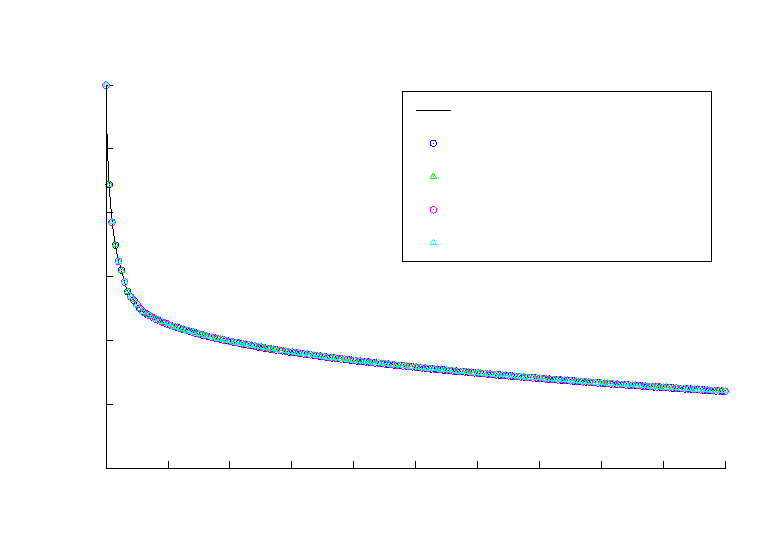
\includegraphics{xenon2_scale}}%
    \gplfronttext
  \end{picture}%
\endgroup
}
	\caption{•••}
	\label{fig:xenon2_scale}
\end{figure}
\begin{figure}
	\centering
	\resizebox{.9\textwidth}{!}{% GNUPLOT: LaTeX picture with Postscript
\begingroup
  \fontfamily{phv}%
  \selectfont
  \makeatletter
  \providecommand\color[2][]{%
    \GenericError{(gnuplot) \space\space\space\@spaces}{%
      Package color not loaded in conjunction with
      terminal option `colourtext'%
    }{See the gnuplot documentation for explanation.%
    }{Either use 'blacktext' in gnuplot or load the package
      color.sty in LaTeX.}%
    \renewcommand\color[2][]{}%
  }%
  \providecommand\includegraphics[2][]{%
    \GenericError{(gnuplot) \space\space\space\@spaces}{%
      Package graphicx or graphics not loaded%
    }{See the gnuplot documentation for explanation.%
    }{The gnuplot epslatex terminal needs graphicx.sty or graphics.sty.}%
    \renewcommand\includegraphics[2][]{}%
  }%
  \providecommand\rotatebox[2]{#2}%
  \@ifundefined{ifGPcolor}{%
    \newif\ifGPcolor
    \GPcolorfalse
  }{}%
  \@ifundefined{ifGPblacktext}{%
    \newif\ifGPblacktext
    \GPblacktexttrue
  }{}%
  % define a \g@addto@macro without @ in the name:
  \let\gplgaddtomacro\g@addto@macro
  % define empty templates for all commands taking text:
  \gdef\gplbacktext{}%
  \gdef\gplfronttext{}%
  \makeatother
  \ifGPblacktext
    % no textcolor at all
    \def\colorrgb#1{}%
    \def\colorgray#1{}%
  \else
    % gray or color?
    \ifGPcolor
      \def\colorrgb#1{\color[rgb]{#1}}%
      \def\colorgray#1{\color[gray]{#1}}%
      \expandafter\def\csname LTw\endcsname{\color{white}}%
      \expandafter\def\csname LTb\endcsname{\color{black}}%
      \expandafter\def\csname LTa\endcsname{\color{black}}%
      \expandafter\def\csname LT0\endcsname{\color[rgb]{1,0,0}}%
      \expandafter\def\csname LT1\endcsname{\color[rgb]{0,1,0}}%
      \expandafter\def\csname LT2\endcsname{\color[rgb]{0,0,1}}%
      \expandafter\def\csname LT3\endcsname{\color[rgb]{1,0,1}}%
      \expandafter\def\csname LT4\endcsname{\color[rgb]{0,1,1}}%
      \expandafter\def\csname LT5\endcsname{\color[rgb]{1,1,0}}%
      \expandafter\def\csname LT6\endcsname{\color[rgb]{0,0,0}}%
      \expandafter\def\csname LT7\endcsname{\color[rgb]{1,0.3,0}}%
      \expandafter\def\csname LT8\endcsname{\color[rgb]{0.5,0.5,0.5}}%
    \else
      % gray
      \def\colorrgb#1{\color{black}}%
      \def\colorgray#1{\color[gray]{#1}}%
      \expandafter\def\csname LTw\endcsname{\color{white}}%
      \expandafter\def\csname LTb\endcsname{\color{black}}%
      \expandafter\def\csname LTa\endcsname{\color{black}}%
      \expandafter\def\csname LT0\endcsname{\color{black}}%
      \expandafter\def\csname LT1\endcsname{\color{black}}%
      \expandafter\def\csname LT2\endcsname{\color{black}}%
      \expandafter\def\csname LT3\endcsname{\color{black}}%
      \expandafter\def\csname LT4\endcsname{\color{black}}%
      \expandafter\def\csname LT5\endcsname{\color{black}}%
      \expandafter\def\csname LT6\endcsname{\color{black}}%
      \expandafter\def\csname LT7\endcsname{\color{black}}%
      \expandafter\def\csname LT8\endcsname{\color{black}}%
    \fi
  \fi
    \setlength{\unitlength}{0.0500bp}%
    \ifx\gptboxheight\undefined%
      \newlength{\gptboxheight}%
      \newlength{\gptboxwidth}%
      \newsavebox{\gptboxtext}%
    \fi%
    \setlength{\fboxrule}{0.5pt}%
    \setlength{\fboxsep}{1pt}%
\begin{picture}(7200.00,5040.00)%
    \gplgaddtomacro\gplbacktext{%
      \csname LTb\endcsname%
      \put(726,704){\makebox(0,0)[r]{\strut{}\footnotesize -6}}%
      \put(726,1316){\makebox(0,0)[r]{\strut{}\footnotesize -5}}%
      \put(726,1929){\makebox(0,0)[r]{\strut{}\footnotesize -4}}%
      \put(726,2542){\makebox(0,0)[r]{\strut{}\footnotesize -3}}%
      \put(726,3154){\makebox(0,0)[r]{\strut{}\footnotesize -2}}%
      \put(726,3767){\makebox(0,0)[r]{\strut{}\footnotesize -1}}%
      \put(726,4379){\makebox(0,0)[r]{\strut{}\footnotesize 0}}%
      \put(1453,484){\makebox(0,0){\strut{}\footnotesize 100}}%
      \put(2047,484){\makebox(0,0){\strut{}\footnotesize 200}}%
      \put(2642,484){\makebox(0,0){\strut{}\footnotesize 300}}%
      \put(3236,484){\makebox(0,0){\strut{}\footnotesize 400}}%
      \put(3831,484){\makebox(0,0){\strut{}\footnotesize 500}}%
      \put(4425,484){\makebox(0,0){\strut{}\footnotesize 600}}%
      \put(5020,484){\makebox(0,0){\strut{}\footnotesize 700}}%
      \put(5614,484){\makebox(0,0){\strut{}\footnotesize 800}}%
      \put(6209,484){\makebox(0,0){\strut{}\footnotesize 900}}%
      \put(6803,484){\makebox(0,0){\strut{}\footnotesize 1000}}%
    }%
    \gplgaddtomacro\gplfronttext{%
      \csname LTb\endcsname%
      \put(352,2541){\rotatebox{-270}{\makebox(0,0){\strut{}\footnotesize Residual 2-norm, log scale}}}%
      \put(3830,154){\makebox(0,0){\strut{}\footnotesize Iteration count}}%
      \put(3830,4709){\makebox(0,0){\strut{}\shortstack{bcsstk18}}}%
      \csname LTb\endcsname%
      \put(4176,4175){\makebox(0,0)[l]{\strut{}\scriptsize GMRES(60)}}%
      \csname LTb\endcsname%
      \put(4176,3856){\makebox(0,0)[l]{\strut{}\begin{minipage}[l]{.95\textwidth} \scriptsize Monomial-GMRES(5,12) \newline \tiny min, max basis rcond \#: 2.02e-44, 2.90e-43\end{minipage}}}%
      \csname LTb\endcsname%
      \put(4176,3537){\makebox(0,0)[l]{\strut{}\begin{minipage}[l]{.95\textwidth} \scriptsize Newton-GMRES(5,12) \newline \tiny min, max basis rcond \#: 1.25e-42, 2.67e-40\end{minipage}}}%
      \csname LTb\endcsname%
      \put(4176,3218){\makebox(0,0)[l]{\strut{}\begin{minipage}[l]{.95\textwidth} \scriptsize Monomial-GMRES(10,6) \newline \tiny min, max basis rcond \#: 8.42e-98, 6.63e-96\end{minipage}}}%
      \csname LTb\endcsname%
      \put(4176,2899){\makebox(0,0)[l]{\strut{}\begin{minipage}[l]{.95\textwidth} \scriptsize Newton-GMRES(10,6) \newline \tiny min, max basis rcond \#: 4.06e-94, 8.41e-90\end{minipage}}}%
    }%
    \gplbacktext
    \put(0,0){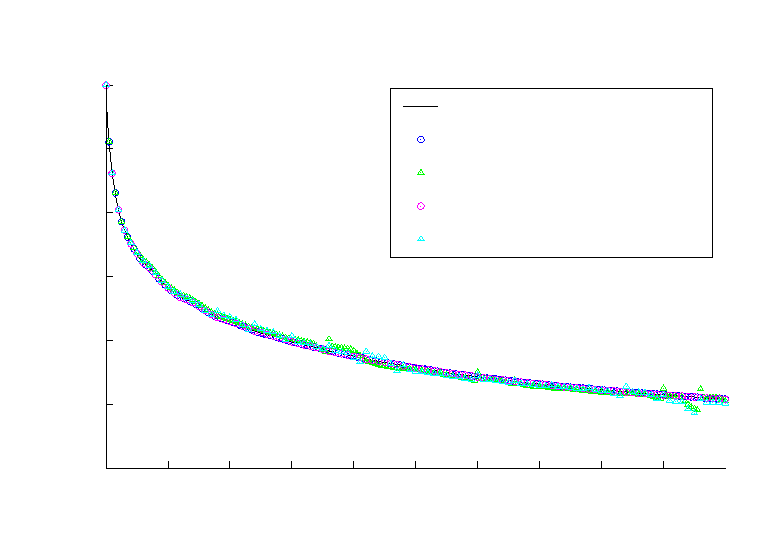
\includegraphics{bcsstk18_noscale}}%
    \gplfronttext
  \end{picture}%
\endgroup
}
	\caption{•••}
	\label{fig:bcsstk18_noscale}
\end{figure}
\begin{figure}
	\centering
	\resizebox{.9\textwidth}{!}{% GNUPLOT: LaTeX picture with Postscript
\begingroup
  \fontfamily{phv}%
  \selectfont
  \makeatletter
  \providecommand\color[2][]{%
    \GenericError{(gnuplot) \space\space\space\@spaces}{%
      Package color not loaded in conjunction with
      terminal option `colourtext'%
    }{See the gnuplot documentation for explanation.%
    }{Either use 'blacktext' in gnuplot or load the package
      color.sty in LaTeX.}%
    \renewcommand\color[2][]{}%
  }%
  \providecommand\includegraphics[2][]{%
    \GenericError{(gnuplot) \space\space\space\@spaces}{%
      Package graphicx or graphics not loaded%
    }{See the gnuplot documentation for explanation.%
    }{The gnuplot epslatex terminal needs graphicx.sty or graphics.sty.}%
    \renewcommand\includegraphics[2][]{}%
  }%
  \providecommand\rotatebox[2]{#2}%
  \@ifundefined{ifGPcolor}{%
    \newif\ifGPcolor
    \GPcolorfalse
  }{}%
  \@ifundefined{ifGPblacktext}{%
    \newif\ifGPblacktext
    \GPblacktexttrue
  }{}%
  % define a \g@addto@macro without @ in the name:
  \let\gplgaddtomacro\g@addto@macro
  % define empty templates for all commands taking text:
  \gdef\gplbacktext{}%
  \gdef\gplfronttext{}%
  \makeatother
  \ifGPblacktext
    % no textcolor at all
    \def\colorrgb#1{}%
    \def\colorgray#1{}%
  \else
    % gray or color?
    \ifGPcolor
      \def\colorrgb#1{\color[rgb]{#1}}%
      \def\colorgray#1{\color[gray]{#1}}%
      \expandafter\def\csname LTw\endcsname{\color{white}}%
      \expandafter\def\csname LTb\endcsname{\color{black}}%
      \expandafter\def\csname LTa\endcsname{\color{black}}%
      \expandafter\def\csname LT0\endcsname{\color[rgb]{1,0,0}}%
      \expandafter\def\csname LT1\endcsname{\color[rgb]{0,1,0}}%
      \expandafter\def\csname LT2\endcsname{\color[rgb]{0,0,1}}%
      \expandafter\def\csname LT3\endcsname{\color[rgb]{1,0,1}}%
      \expandafter\def\csname LT4\endcsname{\color[rgb]{0,1,1}}%
      \expandafter\def\csname LT5\endcsname{\color[rgb]{1,1,0}}%
      \expandafter\def\csname LT6\endcsname{\color[rgb]{0,0,0}}%
      \expandafter\def\csname LT7\endcsname{\color[rgb]{1,0.3,0}}%
      \expandafter\def\csname LT8\endcsname{\color[rgb]{0.5,0.5,0.5}}%
    \else
      % gray
      \def\colorrgb#1{\color{black}}%
      \def\colorgray#1{\color[gray]{#1}}%
      \expandafter\def\csname LTw\endcsname{\color{white}}%
      \expandafter\def\csname LTb\endcsname{\color{black}}%
      \expandafter\def\csname LTa\endcsname{\color{black}}%
      \expandafter\def\csname LT0\endcsname{\color{black}}%
      \expandafter\def\csname LT1\endcsname{\color{black}}%
      \expandafter\def\csname LT2\endcsname{\color{black}}%
      \expandafter\def\csname LT3\endcsname{\color{black}}%
      \expandafter\def\csname LT4\endcsname{\color{black}}%
      \expandafter\def\csname LT5\endcsname{\color{black}}%
      \expandafter\def\csname LT6\endcsname{\color{black}}%
      \expandafter\def\csname LT7\endcsname{\color{black}}%
      \expandafter\def\csname LT8\endcsname{\color{black}}%
    \fi
  \fi
    \setlength{\unitlength}{0.0500bp}%
    \ifx\gptboxheight\undefined%
      \newlength{\gptboxheight}%
      \newlength{\gptboxwidth}%
      \newsavebox{\gptboxtext}%
    \fi%
    \setlength{\fboxrule}{0.5pt}%
    \setlength{\fboxsep}{1pt}%
\begin{picture}(7200.00,5040.00)%
    \gplgaddtomacro\gplbacktext{%
      \csname LTb\endcsname%
      \put(726,704){\makebox(0,0)[r]{\strut{}\footnotesize -6}}%
      \put(726,1316){\makebox(0,0)[r]{\strut{}\footnotesize -5}}%
      \put(726,1929){\makebox(0,0)[r]{\strut{}\footnotesize -4}}%
      \put(726,2542){\makebox(0,0)[r]{\strut{}\footnotesize -3}}%
      \put(726,3154){\makebox(0,0)[r]{\strut{}\footnotesize -2}}%
      \put(726,3767){\makebox(0,0)[r]{\strut{}\footnotesize -1}}%
      \put(726,4379){\makebox(0,0)[r]{\strut{}\footnotesize 0}}%
      \put(1453,484){\makebox(0,0){\strut{}\footnotesize 100}}%
      \put(2047,484){\makebox(0,0){\strut{}\footnotesize 200}}%
      \put(2642,484){\makebox(0,0){\strut{}\footnotesize 300}}%
      \put(3236,484){\makebox(0,0){\strut{}\footnotesize 400}}%
      \put(3831,484){\makebox(0,0){\strut{}\footnotesize 500}}%
      \put(4425,484){\makebox(0,0){\strut{}\footnotesize 600}}%
      \put(5020,484){\makebox(0,0){\strut{}\footnotesize 700}}%
      \put(5614,484){\makebox(0,0){\strut{}\footnotesize 800}}%
      \put(6209,484){\makebox(0,0){\strut{}\footnotesize 900}}%
    }%
    \gplgaddtomacro\gplfronttext{%
      \csname LTb\endcsname%
      \put(352,2541){\rotatebox{-270}{\makebox(0,0){\strut{}\footnotesize Residual 2-norm, log scale}}}%
      \put(3830,154){\makebox(0,0){\strut{}\footnotesize Iteration count}}%
      \put(3830,4709){\makebox(0,0){\strut{}\shortstack{bcsstk18}}}%
      \csname LTb\endcsname%
      \put(4176,4175){\makebox(0,0)[l]{\strut{}\scriptsize GMRES(60)}}%
      \csname LTb\endcsname%
      \put(4176,3856){\makebox(0,0)[l]{\strut{}\begin{minipage}[l]{.95\textwidth} \scriptsize Monomial-GMRES(5,12) \newline \tiny min, max basis rcond \#: 1.67e-04, 1.09e-03\end{minipage}}}%
      \csname LTb\endcsname%
      \put(4176,3537){\makebox(0,0)[l]{\strut{}\begin{minipage}[l]{.95\textwidth} \scriptsize Newton-GMRES(5,12) \newline \tiny min, max basis rcond \#: 1.35e-03, 2.09e-01\end{minipage}}}%
      \csname LTb\endcsname%
      \put(4176,3218){\makebox(0,0)[l]{\strut{}\begin{minipage}[l]{.95\textwidth} \scriptsize Monomial-GMRES(10,6) \newline \tiny min, max basis rcond \#: 6.80e-09, 1.51e-07\end{minipage}}}%
      \csname LTb\endcsname%
      \put(4176,2899){\makebox(0,0)[l]{\strut{}\begin{minipage}[l]{.95\textwidth} \scriptsize Newton-GMRES(10,6) \newline \tiny min, max basis rcond \#: 3.06e-17, 9.12e-03\end{minipage}}}%
    }%
    \gplbacktext
    \put(0,0){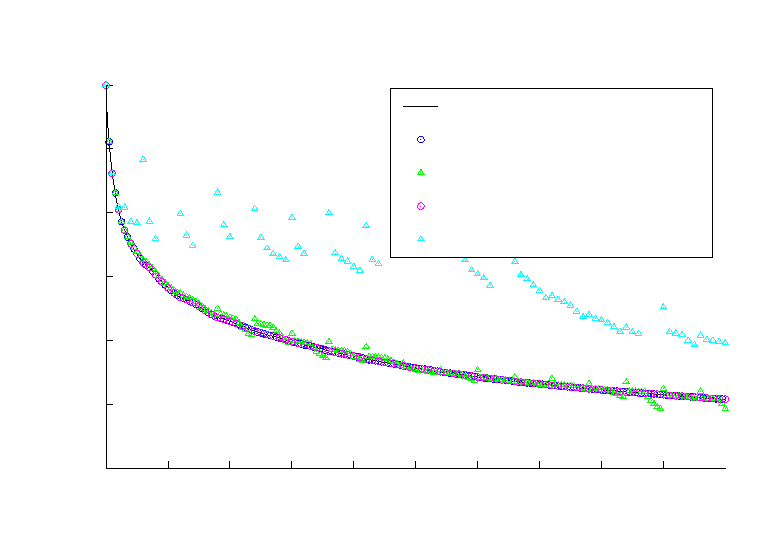
\includegraphics{bcsstk18_scale}}%
    \gplfronttext
  \end{picture}%
\endgroup
}
	\caption{•••}
	\label{fig:bcsstk18_scale}
\end{figure}

\subsection{Performance experiments}
\begin{figure}[H]
	\centering
	\resizebox{1.0\textwidth}{!}{% GNUPLOT: LaTeX picture with Postscript
\begingroup
  \fontfamily{phv}%
  \selectfont
  \makeatletter
  \providecommand\color[2][]{%
    \GenericError{(gnuplot) \space\space\space\@spaces}{%
      Package color not loaded in conjunction with
      terminal option `colourtext'%
    }{See the gnuplot documentation for explanation.%
    }{Either use 'blacktext' in gnuplot or load the package
      color.sty in LaTeX.}%
    \renewcommand\color[2][]{}%
  }%
  \providecommand\includegraphics[2][]{%
    \GenericError{(gnuplot) \space\space\space\@spaces}{%
      Package graphicx or graphics not loaded%
    }{See the gnuplot documentation for explanation.%
    }{The gnuplot epslatex terminal needs graphicx.sty or graphics.sty.}%
    \renewcommand\includegraphics[2][]{}%
  }%
  \providecommand\rotatebox[2]{#2}%
  \@ifundefined{ifGPcolor}{%
    \newif\ifGPcolor
    \GPcolorfalse
  }{}%
  \@ifundefined{ifGPblacktext}{%
    \newif\ifGPblacktext
    \GPblacktexttrue
  }{}%
  % define a \g@addto@macro without @ in the name:
  \let\gplgaddtomacro\g@addto@macro
  % define empty templates for all commands taking text:
  \gdef\gplbacktext{}%
  \gdef\gplfronttext{}%
  \makeatother
  \ifGPblacktext
    % no textcolor at all
    \def\colorrgb#1{}%
    \def\colorgray#1{}%
  \else
    % gray or color?
    \ifGPcolor
      \def\colorrgb#1{\color[rgb]{#1}}%
      \def\colorgray#1{\color[gray]{#1}}%
      \expandafter\def\csname LTw\endcsname{\color{white}}%
      \expandafter\def\csname LTb\endcsname{\color{black}}%
      \expandafter\def\csname LTa\endcsname{\color{black}}%
      \expandafter\def\csname LT0\endcsname{\color[rgb]{1,0,0}}%
      \expandafter\def\csname LT1\endcsname{\color[rgb]{0,1,0}}%
      \expandafter\def\csname LT2\endcsname{\color[rgb]{0,0,1}}%
      \expandafter\def\csname LT3\endcsname{\color[rgb]{1,0,1}}%
      \expandafter\def\csname LT4\endcsname{\color[rgb]{0,1,1}}%
      \expandafter\def\csname LT5\endcsname{\color[rgb]{1,1,0}}%
      \expandafter\def\csname LT6\endcsname{\color[rgb]{0,0,0}}%
      \expandafter\def\csname LT7\endcsname{\color[rgb]{1,0.3,0}}%
      \expandafter\def\csname LT8\endcsname{\color[rgb]{0.5,0.5,0.5}}%
    \else
      % gray
      \def\colorrgb#1{\color{black}}%
      \def\colorgray#1{\color[gray]{#1}}%
      \expandafter\def\csname LTw\endcsname{\color{white}}%
      \expandafter\def\csname LTb\endcsname{\color{black}}%
      \expandafter\def\csname LTa\endcsname{\color{black}}%
      \expandafter\def\csname LT0\endcsname{\color{black}}%
      \expandafter\def\csname LT1\endcsname{\color{black}}%
      \expandafter\def\csname LT2\endcsname{\color{black}}%
      \expandafter\def\csname LT3\endcsname{\color{black}}%
      \expandafter\def\csname LT4\endcsname{\color{black}}%
      \expandafter\def\csname LT5\endcsname{\color{black}}%
      \expandafter\def\csname LT6\endcsname{\color{black}}%
      \expandafter\def\csname LT7\endcsname{\color{black}}%
      \expandafter\def\csname LT8\endcsname{\color{black}}%
    \fi
  \fi
    \setlength{\unitlength}{0.0500bp}%
    \ifx\gptboxheight\undefined%
      \newlength{\gptboxheight}%
      \newlength{\gptboxwidth}%
      \newsavebox{\gptboxtext}%
    \fi%
    \setlength{\fboxrule}{0.5pt}%
    \setlength{\fboxsep}{1pt}%
\begin{picture}(7200.00,5040.00)%
    \gplgaddtomacro\gplbacktext{%
      \csname LTb\endcsname%
      \put(688,512){\makebox(0,0)[r]{\strut{}\footnotesize 0}}%
      \csname LTb\endcsname%
      \put(688,994){\makebox(0,0)[r]{\strut{}\footnotesize 0.5}}%
      \csname LTb\endcsname%
      \put(688,1476){\makebox(0,0)[r]{\strut{}\footnotesize 1}}%
      \csname LTb\endcsname%
      \put(688,1957){\makebox(0,0)[r]{\strut{}\footnotesize 1.5}}%
      \csname LTb\endcsname%
      \put(688,2439){\makebox(0,0)[r]{\strut{}\footnotesize 2}}%
      \csname LTb\endcsname%
      \put(688,2921){\makebox(0,0)[r]{\strut{}\footnotesize 2.5}}%
      \csname LTb\endcsname%
      \put(688,3403){\makebox(0,0)[r]{\strut{}\footnotesize 3}}%
      \csname LTb\endcsname%
      \put(688,3885){\makebox(0,0)[r]{\strut{}\footnotesize 3.5}}%
      \csname LTb\endcsname%
      \put(688,4366){\makebox(0,0)[r]{\strut{}\footnotesize 4}}%
      \csname LTb\endcsname%
      \put(1350,352){\makebox(0,0){\strut{}\footnotesize\,watt1}}%
      \csname LTb\endcsname%
      \put(2619,352){\makebox(0,0){\strut{}\footnotesize\,sherman3}}%
      \csname LTb\endcsname%
      \put(3889,352){\makebox(0,0){\strut{}\footnotesize\,bcsstk18}}%
      \csname LTb\endcsname%
      \put(5159,352){\makebox(0,0){\strut{}\footnotesize\,xenon2}}%
      \csname LTb\endcsname%
      \put(6429,352){\makebox(0,0){\strut{}\footnotesize\,pwtk}}%
    }%
    \gplgaddtomacro\gplfronttext{%
      \csname LTb\endcsname%
      \put(128,2535){\rotatebox{-270}{\makebox(0,0){\strut{}\footnotesize Runtime / runtime(CA-GMRES)}}}%
      \put(3895,112){\makebox(0,0){\strut{}\footnotesize Sparse matrix}}%
      \put(3895,4799){\makebox(0,0){\strut{}\shortstack{\footnotesize\,Runtime\,per\,kernel,\,relative\,to\,CA-GMRES\,with\,best\,s\,and\,restart\,length\\\footnotesize\,for\,all\,test\,matrices\,using\,8\,threads.}}}%
      \csname LTb\endcsname%
      \put(1129,1600){\makebox(0,0){\strut{}1.3x}}%
      \put(2399,1600){\makebox(0,0){\strut{}2.1x}}%
      \put(3669,1600){\makebox(0,0){\strut{}4.0x}}%
      \put(4938,1600){\makebox(0,0){\strut{}2.4x}}%
      \put(6208,1600){\makebox(0,0){\strut{}2.2x}}%
      \csname LTb\endcsname%
      \put(1519,3600){\makebox(0,0)[l]{\strut{}\scriptsize Small dense operations}}%
      \csname LTb\endcsname%
      \put(1519,3760){\makebox(0,0)[l]{\strut{}\scriptsize Block Gram-Schmidt}}%
      \csname LTb\endcsname%
      \put(1519,3920){\makebox(0,0)[l]{\strut{}\scriptsize TSQR}}%
      \csname LTb\endcsname%
      \put(1519,4080){\makebox(0,0)[l]{\strut{}\scriptsize SpMV}}%
      \csname LTb\endcsname%
      \put(1519,4240){\makebox(0,0)[l]{\strut{}\scriptsize INIT}}%
      \csname LTb\endcsname%
      \put(1519,4400){\makebox(0,0)[l]{\strut{}\scriptsize MGS}}%
    }%
    \gplbacktext
    \put(0,0){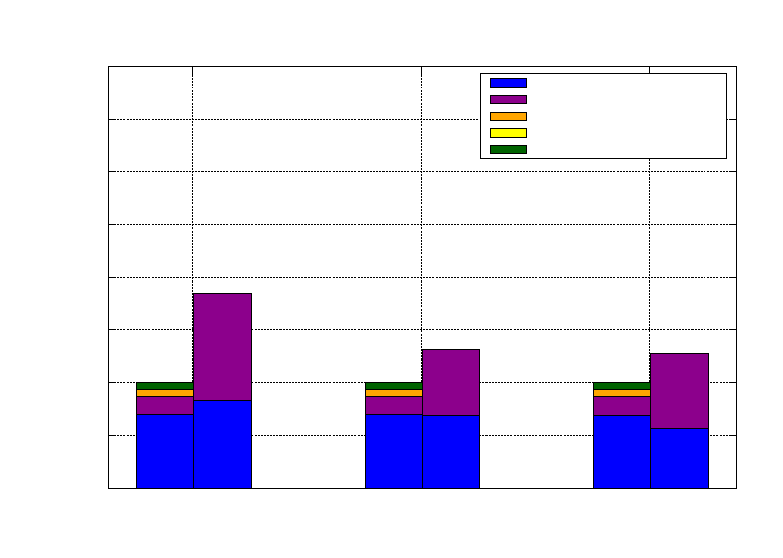
\includegraphics{runtimes_matrices}}%
    \gplfronttext
  \end{picture}%
\endgroup
}
	\caption{left CA-GMRES, right GMRES}
\end{figure}

\subsubsection{Summary}
Conclusion: the MPK is an important kernel and should have been implemented, also restarting with $s$ steps of std. GMRES is not optimal and leaves room for optimization.
\iffalse
compute Ritz values of real upper Hessenberg matrix with LAPACK "DHSEQR()"
\url{http://www.netlib.org/lapack/explore-html/da/dba/group__double_o_t_h_e_rcomputational_gacb35e85b362ce8ccf9d653cc3f8fb89c.html#gacb35e85b362ce8ccf9d653cc3f8fb89c}
\\

Modified Leja ordering \cite{Hoemmen:2010:CKS:1970638} p.291/292\\

Octave code:\\
\url{https://github.com/magnusgrandin/ca-lanczos/blob/master/modified_leja.m}
\fi

\section{Conclusion}

\section*{Krylov subspace methods (summarize this section briefly in introduction)}

\cite{Ascher:2011:FCN:2031413} p.191\\
\begin{itemize}
\item short description:\\
Krylov subspace definition: $\mathcal{K}_k(A, r_0) = span \left\{ r_0, Ar_0, A^2r_0,\ldots,A^{k-1}r_0 \right\}$\\

All iterative methods build and enhance a KSP with every iteration.
\begin{equation*}
\textbf{r}_k = \textbf{r}_0 + \sum_{j=1}^{k} c_jA^j\textbf{r}_0 \quad \to \quad \textbf{x}_k = \textbf{x}_0 + \sum_{j=0}^{k-1} c_{j+1}A^j\textbf{r}_0
\end{equation*}
what is good for the power method, is bad here, bc. vectors are in theory linearly independent but too close to parallel $\to$ in machine arithmetic they become linearly dependent. Need new basis \ldots 
\item Arnoldi \cite{Ascher:2011:FCN:2031413} p.192
\begin{equation*}
AQ_k = Q_{k+1}H_{k+1,k}
\end{equation*}
\item Summary: (\cite{Ascher:2011:FCN:2031413} p. 192)
	\begin{itemize}
	\item 1. construct an orthogonal basis for the Krylov subspace;
	\item 2. define an optimality property;
	\item 3. use an effective preconditioner.
	\end{itemize}
\end{itemize}

\cite{Ascher:2011:FCN:2031413} p.184\\
\begin{itemize}
\item short description: most stable and prominent iterative method, for sym pos def matrices only.
\item Algorithm description (just the basics)
	\begin{itemize}
	\item $\norm{x - x_k}_A = \text{argmin}_{y \in \mathcal{K}_k(A, r_0)}\norm{x - y}_A$\\
	 After $k$-steps, $x_k$ minimizes in the KSP the $A$-norm x - $y$ (only if A is SPD, or else it's not a norm)
	\item follows basic concept: $\textbf{x}_{new} = x_{old} + constant \cdot search direction$ (better version \textit{steepest descent})
	\item $\textbf{r}_k$ is multiple of $q_{k+1}$ ($q$ from Arnoldi; $q$ is not directly used in CG)\\
	$\to$ (1) orthogonal residuals $\textbf{r}_i^T\textbf{r}_k = 0, \quad i < k$\\
	$\to$ (2) $(x_i - x_{i-1})^T A (x_k - x_{k-1}) = 0 \quad \to \quad\Delta \textbf{x}_i^T A \Delta \textbf{x}_k = 0, \quad  i < k$\\
	in other words: the corrections in \textbf{x} are orthogonal in the $A$-inner product, hence the term 'conjugate' in CG. The term 'gradients' comes from minimizing the energy equation/quadratic form:
	\begin{equation*}
	E(x) = \frac{1}{2} \textbf{x}^TA\textbf{x} - b^T\textbf{x} \to min
	\end{equation*}	 
	Set the derivative (gradient) to zero, i.e. $E'(x) = 0$:
	\begin{equation*}
	A\textbf{x} - b = 0
	\end{equation*}
	and we're back to the original problem. So minimizing energies and solving the linear equation $A\textbf{x} = b$ are basically the same.
	\item $H$ is symmetric, and therefore tridiagonal. Arnoldi simplifies to Lanczos $\to$ short 'three-term' recurrences (only have to look at a few previous orthogonal vectors, not all of them).
	\end{itemize}
\item p.191 what about general matrices? Any non-singular matrix $A$ can be transformed into SPD matrix via $A^TA$ $\to$ bad condition number $\kappa (A)$.\\

\{The condition number of the matrix $A^TA$ is the square of the condition number of $A$ [\ldots] A large condition number both increases the number of iterations required and limits the accuracy to which a solution can be obtained. \cite{press92a} p. 89 (2.7.40)\}
consider Krylov subspace methods that are directly based on general matrix $A$ $\to$ GMRES
\end{itemize}

\subsection*{GMRES (summarize this section briefly in introduction)}
\begin{itemize}
\item short description: general form of MINRES (=like CG it is only for symmetric matrices, but must not be PD) MINRES minimizes $\norm{\textbf{r}_k}_2$ and CG minimizes energy norm of the residual $\norm{\textbf{r}_k}_{A^{-1}}$ or the energy norm of the error $\norm{\textbf{x}^* - \textbf{x}_k}_A$ respectively. \cite{Ascher:2011:FCN:2031413} (p. 198)
\item algorithm description:
\item $\norm{b - A\textbf{x}_k}_2 = argmin_{y \in \mathcal{K}_k(A, r_0)}\norm{b - Ay}_2$\\
	 After $k$-steps, $\textbf{x}_k$ minimizes in the KSP the $\ell^2$-norm $b - Ay$
\item GMRES vs. CG:
\begin{itemize}
\item CG forces the residual $\textbf{r}_k$ to be orthogonal to the Krylov subspace $\mathcal{K}_k(A, r_0)$;
\item GMRES seeks the residual with minimum $\ell_2$-norm within the Krylov subspace.
\end{itemize}
\item Summary:\\
The main components of a single iteration of GMRES are
\begin{enumerate}
	\item perform a step of the Arnoldi process;
	\item update the QR factorization of the updated upper Hessenberg matrix;
	\item solve the resulting least squares problem.
	\end{enumerate}
\end{itemize}

\bibliographystyle{plain}
\bibliography{BSc_Ernstbrunner_01403753}
 \listofalgorithms
\begin{appendices}
\section*{Appendix A}
discussion of test matrices
\end{appendices}
\end{document}
% End of document.